\documentclass[12pt,twoside,a4paper,draft]{article} 
\usepackage{fullpage}
\usepackage{graphicx}
\usepackage{natbib}
\usepackage{maple2e}
\usepackage[leqno,fleqn]{amsmath}
\usepackage[polish,english]{babel} 
\usepackage[plmath,MeX]{polski} 
\usepackage[cp1250]{inputenc}
\usepackage[font=footnotesize,format=plain,labelfont=bf,up,textfont=it,up]{caption}
\def\emptyline{\vspace{12pt}}
\pretolerance=350
\pagenumbering{arabic}
\graphicspath{{./img/}} % A path to the graphics directory
\numberwithin{equation}{subsection}
\numberwithin{figure}{subsection}
\selectlanguage{english} % We choose the autogenerated texts' language to be english

%\addtolength{\hoffset}{-1.0cm}
\addtolength{\voffset}{-1.0cm}
%\addtolength{\textwidth}{2cm}
\linespread{1.7} %interline

\pagestyle{plain}
\title{Numerical evaluation of the Hilbert transform used to better understand 
and solve the Kramers-Kronig relations in nonlinear optics}
 \author{Krzysztof Parjaszewski}
 \date{}
\def\Xint#1{\mathchoice
{\XXint\displaystyle\textstyle{#1}}%
{\XXint\textstyle\scriptstyle{#1}}%
{\XXint\scriptstyle\scriptscriptstyle{#1}}%
{\XXint\scriptscriptstyle\scriptscriptstyle{#1}}%
\!\int}
\def\XXint#1#2#3{{\setbox0=\hbox{$#1{#2#3}{\int}$ }
\vcenter{\hbox{$#2#3$ }}\kern-.6\wd0}}
\def\ddashint{\Xint=}
\def\dashint{\Xint-}
\begin{document}
\maketitle
\paragraph{}

\subsubsection*{Dedication}


To my Family.


\section*{Abstract}
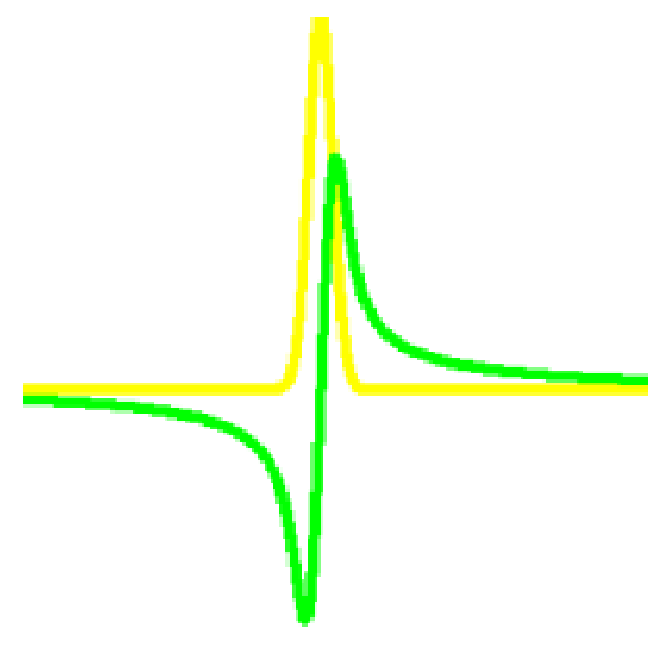
\includegraphics{img/title.eps}
\paragraph
The motivation for this work comes from the real problem state by
physicists and chemists building the valid theoretical models to
describe the interaction between light and matter due to both
non-intensive and intensive light radiation. The starting point is the
fundamental physical law - the causality principle - which states that
the effect cannot precede the cause. This simple assumption leads us
the Titchmarsh theorem about the Hilbert Transform - and together with
advanced signal response-theory we can investigate the properties of
the medium response to the periodic input signal - both in time and
frequency domain. Modifications of the Hilbert Transform for the
optical susceptibility 
$\chi (\omega )$ are known as the Kramers-Kronig relations - which are defined for
both real and imaginary part of susceptibility in the frequency-domain:
$$\Re (\chi (\omega ))=\frac {2\,\int _{ - \infty }^{\infty }
\frac {\Omega \,\Im (\chi (\Omega ))}{\Omega ^{2} - \omega ^{2}}
\,d\Omega }{\pi }$$

$$\Im (\chi (\omega ))=\frac {2\,\omega \,\int _{ - \infty }^{
\infty }\frac {\Re (\chi (\Omega ))}{\Omega ^{2} - \omega ^{2}}\,
d\Omega }{\pi }$$

where the integration uses the Cauchy principal value method. In the
thesis we handle two problems. First concerns numerical problems with
calculation of such singular and improper integral. The second problem
concerns the questions stated by physicists - how to properly use this
mathematical tools in a typical experiment and model construction in
optical research. We present the comparison of several implementations
of numerical calculations of the Hilbert transform:
\begin{itemize} \label{used_methods}
 \item Numerical trapezoidal rule mixed with the Simpson's rule and the
cubic interpolation
 \item Newton-Cotes qudrature of sixth degree
 \item Clenshaw-Curtis quadrature
 \item Hilbert transform based on fast Hartley transforms
 \item method based on approximation with the orthonormal Hermite
polynomials and Hermite functions
 \item method based on approximation with the Fourier series.
\end{itemize}
We also test the out-of-the-box MATLAB-implemented routines:
\begin{itemize} \label{matlab_methods}
  \item quadgk()
  \item hilbert() - based on FFT
\end{itemize}
The given physical models for both linear and nonlinear optics are
analysized and validated. We formulate good practises for scientists
interested in subject of optical experiments. Finally we made the
conclusions about the numerical stability, advantages and
disadvantages of developed implementations in further research in
nonlinear optics.

\emptyline

\subsection*{Keywords}


numerical analysis, nonlinear optics, Hilbert transform,
Kramers-Kronig relations, optical dispersion relations


\subsection*{Promotors}

\subsubsection*{Nonlinear optics:}


\textbf{Professor Marek Samo�}



Institute of Physical and Theoretical Chemistry \\
Wroclaw University of Technology, PL-50-370 Wroclaw \\
Wybrzeze Wyspianskiego 27, Poland \\
+48-71-320-4466 | E-mail: Marek.Samoc@pwr.wroc.pl



\subsubsection*{Numerical analysis:}



\textbf{Pawe� Keller PhD}



Group of Numerical Methods, Institute of Computer Science \\
University of Wroclaw, PL-50-383 Wroclaw \\
ul. Joliot-Curie 15, Poland \\
+48-71-375-7813 | E-mail: Pawel.Keller@ii.uni.wroc.pl


\emptyline

\subsubsection*{Author}



\textbf{Krzysztof Parjaszewski}



Institute of Computer Science \\
University of Wroc�aw, PL-50-383 Wroc�aw \\
ul. Joliot-Curie 15, Poland \\
+48-660-070-043 | E-mail: Krzysztof.Parjaszewski@Gmail.Com




\subsubsection*{Reviewer}


\textbf{Professor Stanislaw Lewanowicz}



Group of Numerical Methods, Institute of Computer Science \\
University of Wroclaw, PL-50-383 Wroclaw
ul. Joliot-Curie 15, Poland \\
+48-71-375-7813 | E-mail: Stanislaw.Lewanowicz@ii.uni.wroc.pl



\section{Introduction to the nonlinear optics (understanding)}

\subsection{What is this thesis about?}



This thesis is a small step for better understanding the nature of
light and its interaction with matter.





The main motivation and subject of this thesis is the application of
numerical methods for better modelling and understanding the physical
models in nonlinear optics. The main experiment used during the work
on this thesis has been conducted with the Z-Scan technique on a
high-energy femtosecond laser system consisting of a Quantronix
Integra-C amplifier operating at 800 nm and a Quantronix-Palitra-FS
BIBO crystal-based optical parametric amplifier which allows us to
modify the output wavelength in range of \symbol{126}650nm up to
\symbol{126}2000nm. The laser pulses were of \symbol{126}130 fs length
and 1kHz repetition rate. Experiments were performed at the Wroclaw
University of Technology at the Institute of Physical and Theoretical
Chemistry. Numerical calculations were performed on a simple personal
laptop within MATLAB and Maple environment.





The main numerical results concern the usage of the the Kramers-Kronig
relations and the discussion about its application for nonlinear
optics. Firstly the simple linear Kramers-Kronig relation has been
derived and reviewed, then is has been developed into simple nonlinear
case. Next the perturbative approach and other modifications in
discussed model are reviewed. In each of these examples, an attention
is paid to the numerical issues. The constructed numerical
calculations are compared and discussed and further good practices for
physicists and chemists are formulated.





The subject of this thesis is not accidential - in last twenty years
the global interest on light application in modern devices - including
the construction of super-fast all-optical computers - increases. In
Poland - the nanophotonics research is developing in several
scientific centers and Wroclaw is one of the leading ones.
To review both with Prof. MS and Dr PK.

\subsection{What is the nonlinear optics?}
In mathematics a linear function f satisfies both of the following
properties:
\begin{subequations}  \label{eq:linear_optics}
 \begin{equation}  \label{eq:nlo_additivity}  
   \text{additivity:\,} \, \forall \, x, y : f(x+y) = f(x) + f(y)
  \end{equation}
  \begin{equation} \label{eq:nlo_homogeneity}   
   \text{homogeneity:\,} \, \forall \, \alpha : f(\alpha\,x) = \alpha\,f(x)
  \end{equation}
\end{subequations}
Sometimes another name for a function is used: ''system''. The nonlinear
system is so a function which does not satisfies both additivity and
homogenity simultaneosly. Another definition says that nonlinear
system does not follow the superposition rule. The main area of
interest for nonlinear optics is the behaviour of optical wave in a
nonlinear medium. In such a case the superposition principle no longer
holds, and therefore the response of a system/function depends
nonlinearly on the input signal. In practice the nonlinearity shows
only with very high intensities of light, so this theory is only
applied to high intensity devices - such as modern lasers or optical
fibers. Nonlinear optics is strongly related to physics, biology and
chemistry but also mathematics and computer science, because modelling
the light behaviour is an open problem still being solved
interdisciplinary - what has been showed on the
\ref{fig:nonlinear_optics}:\textit{}



\begin{figure} 
 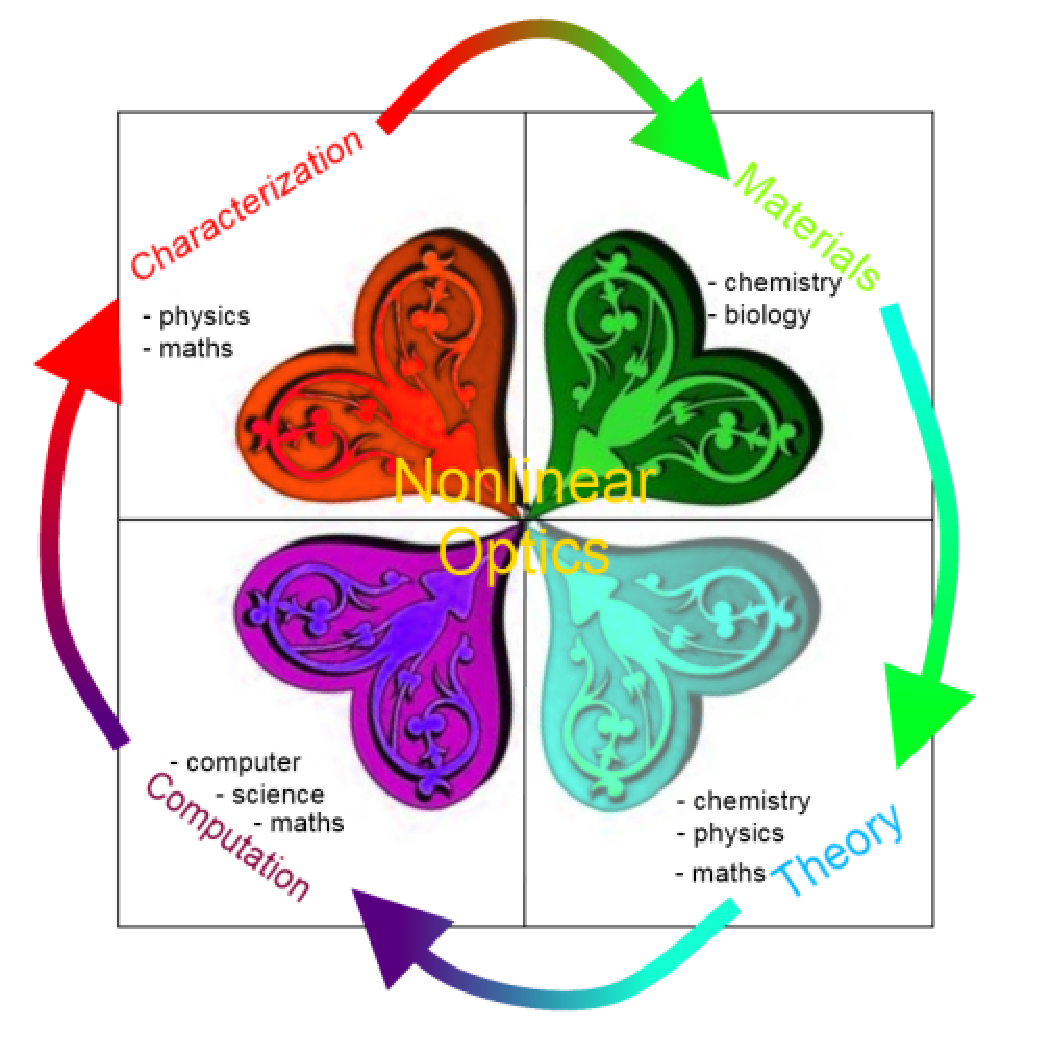
\includegraphics{nlo.eps}
 \caption{Nonlinear optics derives from many foundamentary
disciplines: biology, chemistry, math, physics and computer science\label{fig:nonlinear_optics}}
\end{figure}


An comprehensive, well prepared introduction to the nonlinear optics
can be found in the \textit{Nonlinear Optics} written by Robert Boyd
[2].

\subsection{What are the most important nonlinear optical
properties and phenomena?}

Experiments, which investigates the nonlinear nature of light are
similar to those in classical optics, but they differ in the intensity
of source radiation. Under the influence of the powerful and ultrafast
lasers all optical properties and phenomena such as refraction,
diffraction, interference, dyspersion, scattering etc. tend to modify.
With pulses lasting from 10 femtoseconds up to 10 picoseconds and
energy per pulse between 1 mJ and 1000 mJ laser produces a single
pulse with a power of giga-, tera- or even perawatts. Influenced by a
such huge power of the light beam - matter shows its nonlinear
properties. 

We define the following classification of the linear and nonlinear
optical phenomena:
- linear phenomena
- second order nonlinear phenomena
- third order nonlinear phenomena
- nonlinear phenomena of higher orders

\includegraphics{img/opt_phenom.eps}


{Picture 1.3.1 - schematic diagram of nonlinear optical phenomena -
the input wavelength differs from the output signal, which occurs only
for strong optical signals.}





The basis of such classification is the equation defined for the
electric polarization by the classical electromagnetism. The
polarization density vector $[\frac {C}{m^{2}}]$ is approximated by 
Taylor series: 



(1.3.1) 
$\frac {{P_{i}}}{{\varepsilon _{0}}}=\frac {{P_{i}}(0)}{{
\varepsilon _{0}}} + (\sum _{j=1}^{3}\,{\chi _{\mathit{ij}}}^{[1]
}\,{E_{j}}) + (\sum _{k=1}^{3}\,(\sum _{j=1}^{3}\,{\chi _{
\mathit{ijk}}}^{[2]}\,{E_{j}}\,{E_{k}})) +  \left(  \! \sum _{l=1
}^{3}\,(\sum _{k=1}^{3}\,(\sum _{j=1}^{3}\,{\chi _{\mathit{ijkl}}
}^{[3]}\,{E_{j}}\,{E_{k}}\,{E_{l}})) \!  \right) $ + ...    for 
$i=1, \,2, \,3$
with omission of 
$\frac {1}{n\mathrm{!}}$
factors in the power expansion,





where:



\mapleinline{inert}{2d}{chi^[1];}{%
$\chi ^{[1]}$%
} : 
\mapleinline{inert}{2d}{[m^2/(V^2)];}{%
$[\frac {m^{2}}{V^{2}}]$%
} - the linear susceptibility tensor;



\mapleinline{inert}{2d}{chi^[2];}{%
$\chi ^{[2]}$%
} : 
\mapleinline{inert}{2d}{[m^2/(V^2)];}{%
$[\frac {m^{2}}{V^{2}}]$%
} - the second order nonlinear susceptibility tensor - responsible for
phenomena such as electro-optic rectification (EOR), second-harmonic
generation (SHG), generation of sum and differential frequencies (SFG
and DFG) and Pockels electro-optic effect;



\mapleinline{inert}{2d}{chi^[3];}{%
$\chi ^{[3]}$%
} : 
\mapleinline{inert}{2d}{[m^2/(V^2)];}{%
$[\frac {m^{2}}{V^{2}}]$%
} - the third order nonlinear susceptibility tensor - responsible for
phehonema such as intensity dependent refractive index (IDRI), third
harmonic generation (THG), stimulated brillouin scattering (SBS),
stimulated raman scattering (SRS), degenerate four waves mixing (DFWM)
and nonlinear absorption [3]. 





The intensity dependent refractive index (IDRI) results from the
resonant response of an atomic system and can be described by the
equation:





(1.3.2) 
\mapleinline{inert}{2d}{n = n[0]+[n[2]]*`<,>`(E^2);}{%
$n={n_{0}} + [{n_{2}}]\,\langle E^{2}\rangle $%
},





where: 



\mapleinline{inert}{2d}{n[0];}{%
${n_{0}}$%
} - the weak-field refractive index;



\mapleinline{inert}{2d}{[n[2]];}{%
$[{n_{2}}]$%
} - the second order index of refraction;



\mapleinline{inert}{2d}{`<,>`(E^2);}{%
$\langle E^{2}\rangle $%
} - means the time average around E.





\mapleinline{inert}{2d}{[n[2]];}{%
$[{n_{2}}]$%
} is a new optical constant which describes the increasement of the
refractive index in the relation to the intensity of optical signal. 





The arisement of the refractive index is sometimes called the optical
Kerr effect. It is a similar effect to the Kerr electro-optic effect,
which is a modification of the refraction index under the influence of
the strong electric field applied to the medium. In the optical case
the change of refraction index comes only from the influence of very
intensive light beam, typically from the laser system. The theory
beneath this effect has its roots in some quantum mechanics effects
(e.g. the dynamic Burstein-Moss effect) and as the nanophotonics is
relatively new scientific domain, there are only more or less
confirmed hypothesis being under investigation.





Several effects come as the result from the indensity dependent
refractive index:
a) self-focusing of light - focusing the light beam within the
nonlinear medium



b) two beam coupling - is the energy transfer between two light beams
interaction within the nonlinear medium



c) optical phase conjugation - is responsible for reversing the
typical abberation effects 
d) all-optical switching - is the very interesting effect which allows
to control the flow of one beam by another. In other words it is a
control of light by light.  





The nonlinear absorption may concerns the absorption of energy from
two or more photons influencing matter in the very same moment of time
or the absorption of light under the heavy light intensity. Both
linear and nonlinear absorption process has the property of spatial
selectivity, which means that the with different angle of light beam
incidenting on matter we get different absorption coefficients - which
is related to the tensor nature of the optical susceptibility. Also
the polarization geometry of the light beam plays important role here
[5].

\textit{Description of determination the nonlinear optical properties
and describing the NLO phenomena in several sentenses.}




\subsection{Why is nonlinear optics so important?}



Nonlinear optics is the widely investigated area in nanophotonics,
because a material with a high nonlinear refractive index will be a
key to to build an all-optical-transistor and such device should work
as an all-optical logic gate. That will lead us to create the
ultra-fast optical devices, for instance the fotonic computer - where
instead of electrons, fotons will be used to perform computations with
a very high speed. Some scientists suggest that the taming of
all-optical-switching phenomenom is the Holy Grail of modern photonics
[3].





On the other hand - the nonlinear absorption, which is strongly
related to the nonlinear refraction index - is an important obstacle
to build such a fast all-optical-device. Despite ot that, nonlinear
absorption still may be very useful in nanofabrication, biophotonics,
microscopy, information storage and other technologies using short
laser pulses[4]. 





The interest in nonlinear optics comes from both the basic research
and industry. The basic research and fundamental questions in material
research concerns the nature of light, optical properties of
molecules, the strength and properties of chemical bonds and theory to
determine both linear and nonlinear optical properties insead of
performing myriads of experiments. The industrial research interests
in nonlinear optics are mostly focused in the area of developing new
optical devices (detectors, engines, logic gates, fibers, lasers and
more) and the usage of intensive light beams for various types of
screening and determing the 3D information about the geometrical of
the investigated material.





\textit{Description of} \textit{the most expected results of
understanding the nonlinear optics.}




\subsection{Why should we use Kramers Kronig relations here?}



Kramers Kronig relations are the fundamental tools in the exploration
of the material optical properties and together with other classical
physics and quantum mechanics predictions can be used to construct and
validate theoretical models. They are originated from the most basic
but also very important law in physics - the causality principle. From
the philosophical perspective it states that each effect must be
preceded by a cause. In computer science this principle is somehow
paraphrased in a discussion of formal deterministic and
nondeterministic automatas. We believe that only deterministic
automatas really exist. 





(1.5.1a) 
\mapleinline{inert}{2d}{Psi(t);}{%
$\Psi (t)$%
} = 
\mapleinline{inert}{2d}{IFT(Psi(omega));}{%
$\mathrm{IFT}(\Psi (\omega ))$%
} 
(1.5.1b) '' t \TEXTsymbol{<} 0 : 
\mapleinline{inert}{2d}{Psi(t) = 0;}{%
$\Psi (t)=0$%
} 





The causability principle looks obvious, but in the field of nonlinear
optics - combined together with the application of the inverse Fourier
transform of any nonlinear quantity spectrum: 
\mapleinline{inert}{2d}{Psi(omega);}{%
$\Psi (\omega )$%
}, \textbf{R} ' 
\mapleinline{inert}{2d}{omega;}{%
$\omega $%
}  - it states that the time-domain signal 
\mapleinline{inert}{2d}{Psi(t);}{%
$\Psi (t)$%
} calculated with (1.5.1a) from frequency-domain must equal zero for
any negative time argument. This statement can be used in validation
of any spectrum 
\mapleinline{inert}{2d}{Psi(omega);}{%
$\Psi (\omega )$%
}, \textbf{R} ' 
\mapleinline{inert}{2d}{omega;}{%
$\omega $%
} - what is important when we only measure the physical quantity in a
specific range \$ 
\mapleinline{inert}{2d}{a,b:;}{%
$a, \,b$%
} : 
\mapleinline{inert}{2d}{a < omega;}{%
$a < \omega $%
} and 
\mapleinline{inert}{2d}{omega < b;}{%
$\omega  < b$%
}. We simply cannot measure the whole real spectrum \textbf{R} ' 
\mapleinline{inert}{2d}{omega;}{%
$\omega $%
} and in this case we need to perform the validation of approximated
or assumed spectrum 
\mapleinline{inert}{2d}{Psi(omega);}{%
$\Psi (\omega )$%
}.





Kramers Kronig relations - which will be derived in the following
chapter - connects the real and imaginary part of the Fourier
transform of valid response signal. It is said that one can derive the
real part of the determined spectrum 
\mapleinline{inert}{2d}{Psi(omega);}{%
$\Psi (\omega )$%
}. What is even more important - this relation is bidirectional - so
with the Kramers Kronig relations one can derive the imaginary part
from real. This hypothesis has been formulated in 1948 by Edward
Charles Titchmarsh - with the tacit assumption, that both 
\mapleinline{inert}{2d}{Psi(t);}{%
$\Psi (t)$%
} and 
\mapleinline{inert}{2d}{Psi(omega);}{%
$\Psi (\omega )$%
} are the square-integrable functions and more - the 
\mapleinline{inert}{2d}{Psi(omega);}{%
$\Psi (\omega )$%
} holomorphic in the upper-plane. This simple theorem - is widely
investigated area in both the nonlinear and linear optics - to connect
the refraction index togheter with absorption coefficient, which are
th real and imaginary parts of the optical susceptibility
respectively.





\textit{Just few words about the hopes of using K-K relations also in
nonlinear optics.}




\subsubsection*{Notes}



1. ''Znajomo�� pe�nej funkcji dielektrycznej 
\mapleinline{inert}{2d}{epsilon(omega) = epsilon[1](omega)+i*epsilon[2](omega);}{%
$\varepsilon (\omega )={\varepsilon _{1}}(\omega ) + i\,{
\varepsilon _{2}}(\omega )$%
} daje nam klasycznie pe�ny opis zjawisk towarzysz�cych rozchodzeniu
si� fali elektromagnetycznej w materii.''
2. Teori� fitowania lorentzian�w opisuje regresja nieliniowa.





\textit{Some notes in both polish and english.}




\section{Problem definition (understanding)}

\subsection{Linear model}



Basically in the linear optical model we assume, that the response of
a medium depends linearly on the input. The similar presumption is
made in many fields of physics - for instance in magnetostatics we
linearly connect the current density \textbf{J} with the electric
field \textbf{E} vector multiplied by a conductivity parameter 
\mapleinline{inert}{2d}{sigma;}{%
$\sigma $%
} - which is called the Kirchhoff's reformulation of the Ohm's Law:





(2.1.1) \textbf{J} = 
\mapleinline{inert}{2d}{sigma;}{%
$\sigma $%
} \textbf{E}





As it will be shown later, such relations hold for sufficiently small
intensities - but the definition of 'sufficiently small' will not be
further specified. In the time-domain it is stated that an external
sinusoidal electromagnetic radiation of a light beam - \textbf{the
input} - is defined by a field vector:





(2.1.2) \textbf{E}(\textbf{r}, t) = 
\mapleinline{inert}{2d}{1/r;}{%
$\frac {1}{r}$%
} 
\mapleinline{inert}{2d}{E[0];}{%
${E_{0}}$%
}cos(\textbf{k r - 
\mapleinline{inert}{2d}{omega;}{%
$\omega $%
}} t + 
\mapleinline{inert}{2d}{phi;}{%
$\phi $%
}), 





where:
\textit{\textbf{{\small k - wave vector (radians per meter)
r - position vector (meters) 
t - time (seconds)}}}



\mapleinline{inert}{2d}{omega;}{%
$\omega $%
} - \textit{{\small angular frequency (radians per second)}}



\mapleinline{inert}{2d}{phi;}{%
$\phi $%
} - \textit{{\small phase shift (radians). }}





\textbf{The output} - reponse in the form of polarization vector can
be described using the linear response theory - which is the
simplification of the Volterra series that takes only the leading
order term can be described as the following convolution:





(2.1.3) 
\mapleinline{inert}{2d}{P[1,i];}{%
${P_{1, \,i}}$%
}(\textbf{r}, t) = 
\mapleinline{inert}{2d}{epsilon[0]*sum(int(int(G[1,i,j](p-r,s-t)*E[1,j](p,s),p),s = -infinity
.. infinity),j = 1 .. 3);}{%
${\varepsilon _{0}}\, \left(  \! \sum _{j=1}^{3}\,\int _{ - 
\infty }^{\infty }\int {G_{1, \,i, \,j}}(p - r, \,s - t)\,{E_{1, 
\,j}}(p, \,s)\,dp\,ds \!  \right) $%
}  with the inner integral made through the Euclidean space 
\mapleinline{inert}{2d}{R^3;}{%
$R^{3}$%
}.[6]





where:
1 - the '1' index states for linear property of any investigated value
\mapleinline{inert}{2d}{P[1,i];}{%
${P_{1, \,i}}$%
} - 3x1 real linear polarization tensor (vector) in a
spacetime-domain, i stays for chosen spatial coordinate (x, y or z) [
\mapleinline{inert}{2d}{C/(m^2);}{%
$\frac {C}{m^{2}}$%
}]
\mapleinline{inert}{2d}{G[1,i,j];}{%
${G_{1, \,i, \,j}}$%
} - 3x3 real susceptibility tensor (matrix) defined by a linear Green
function in a spacetime-domain \cite{fakiszscan}
\mapleinline{inert}{2d}{E[1,j];}{%
${E_{1, \,j}}$%
} - 3x1 real electric field tensor (vector) in a spacetime-domain [
\mapleinline{inert}{2d}{V/m;}{%
$\frac {V}{m}$%
}]



\mapleinline{inert}{2d}{epsilon[0];}{%
${\varepsilon _{0}}$%
} - electric permittivity of free space $8.854187817620 x$ 
\mapleinline{inert}{2d}{10^(-12);}{%
$10^{( - 12)}$%
}  [
\mapleinline{inert}{2d}{C/(V*m);}{%
$\frac {C}{V\,m}$%
}]
\textit{\textbf{{\small r - position vector (meters) 
t - time (seconds)}}}





Even such linear equation is only the simplification, because we do
not assume the local field corrections [7]. It seems to be an
reasonable assumption as long as we emphasize the macroscopic
character of polarization. Only in case of constructing very small
devices or synthesizing small particles - we shall take the local
field interaction into account. Investigation of the properties of the
susceptibility tensor both in time-domain and frequency-domain will be
the main part of considerations in this thesis - it is also widely
discussed topic in the literature [2,8,9,10,11]





The Fourier transform allows us to change the polarization equation
(2.1.3) from time-domain to frequency-domain:





(2.1.4) 
\mapleinline{inert}{2d}{Phi;}{%
$\Phi $%
}\textbf{\{F}[
\mapleinline{inert}{2d}{P[1,i];}{%
${P_{1, \,i}}$%
}(\textbf{r}, t)]\} = 
\mapleinline{inert}{2d}{P[1,i];}{%
${P_{1, \,i}}$%
}(\textbf{k}, 
\mapleinline{inert}{2d}{omega;}{%
$\omega $%
})





where:
\mapleinline{inert}{2d}{Phi;}{%
$\Phi $%
} - Fourier transform operation in 3D space domain
\textbf{F} - Fourier transform operation in time domain
\mapleinline{inert}{2d}{P[1,i];}{%
${P_{1, \,i}}$%
}(\textbf{k}, 
\mapleinline{inert}{2d}{omega;}{%
$\omega $%
})\textbf{ - }3x1 complex linear polarization tensor (vector) in a
wavefrequency-domain, i stays for chosen spatial coordinate (x, y or
z) [
\mapleinline{inert}{2d}{C/(m^2);}{%
$\frac {C}{m^{2}}$%
}]\textbf{
k} - 3x1 wave tensor (vector) of the electromagnetic field [
\mapleinline{inert}{2d}{1/m;}{%
$\frac {1}{m}$%
}]
\mapleinline{inert}{2d}{omega;}{%
$\omega $%
} - angular frequency of the electromagnetic field [
\mapleinline{inert}{2d}{rad/s;}{%
$\frac {\mathit{rad}}{s}$%
}],





Due the convolution theorem [12] the Fourier transform applied to the
convolution of two given functions equals the simple multiplication of
two Fourier transforms:
(2.1.5) 
\mapleinline{inert}{2d}{Phi;}{%
$\Phi $%
}\textbf{\{F}[
\mapleinline{inert}{2d}{epsilon[0]*sum(int(int(G[1,i,j](p-r,s-t)*E[1,j](p,s),p),s = -infinity
.. infinity),j = 1 .. 3);}{%
${\varepsilon _{0}}\, \left(  \! \sum _{j=1}^{3}\,\int _{ - 
\infty }^{\infty }\int {G_{1, \,i, \,j}}(p - r, \,s - t)\,{E_{1, 
\,j}}(p, \,s)\,dp\,ds \!  \right) $%
}]\} =
\mapleinline{inert}{2d}{epsilon[0]*sum(chi[1,i,j](k,omega)*E[1,j](k,omega),j = 1 .. 3);}{%
${\varepsilon _{0}}\,(\sum _{j=1}^{3}\,{\chi _{1, \,i, \,j}}(k, 
\,\omega )\,{E_{1, \,j}}(k, \,\omega ))$%
}





where:
\mapleinline{inert}{2d}{Phi;}{%
$\Phi $%
} - Fourier transform operation in 3D space domain
\textbf{F} - Fourier transform operation in time domain
\mapleinline{inert}{2d}{chi[1,i,j];}{%
${\chi _{1, \,i, \,j}}$%
}(\textbf{k}, 
\mapleinline{inert}{2d}{omega;}{%
$\omega $%
}) - 3x3 complex susceptibility tensor (matrix) in a
wavefrequency-domain [1] 
\mapleinline{inert}{2d}{E[1,j];}{%
${E_{1, \,j}}$%
}(\textbf{k}, 
\mapleinline{inert}{2d}{omega;}{%
$\omega $%
}) - 3x1 complex electric field tensor (vector) in a
wavefrequency-domain [
\mapleinline{inert}{2d}{V/m;}{%
$\frac {V}{m}$%
}]





From (2.1.4) and (2.1.5) we get:





(2.1.6) 
\mapleinline{inert}{2d}{P[1,i];}{%
${P_{1, \,i}}$%
}(\textbf{k}, 
\mapleinline{inert}{2d}{omega;}{%
$\omega $%
}) = 
\mapleinline{inert}{2d}{epsilon[0]*sum(chi[1,i,j](k,omega)*E[1,j](k,omega),j = 1 .. 3);}{%
${\varepsilon _{0}}\,(\sum _{j=1}^{3}\,{\chi _{1, \,i, \,j}}(k, 
\,\omega )\,{E_{1, \,j}}(k, \,\omega ))$%
}





which seems to be a simpler equation - so from now we will use the
wavefrequency-domain. We will no be getting further into the physical
details of the optical susceptibility theory. For our interests it is
worth stressing, that the 
\mapleinline{inert}{2d}{G[1,i,j];}{%
${G_{1, \,i, \,j}}$%
} - 3x3 real susceptibility tensor (matrix) defined by a linear Green
function in a spacetime-domain follows the following rules:





(2.1.7a) + the causality principle '' 
\mapleinline{inert}{2d}{t < 0;}{%
$t < 0$%
} : 
\mapleinline{inert}{2d}{G[1,i,j];}{%
${G_{1, \,i, \,j}}$%
}(\textbf{r}, t) = 0
(2.1.8a) + the convservation of energy law: '' \textbf{r }:
\mapleinline{inert}{2d}{int(G[1,i,j](r,t),t = -infinity .. infinity) < infinity;}{%
$\int _{ - \infty }^{\infty }{G_{1, \,i, \,j}}(r, \,t)\,dt < 
\infty $%
}





The Fourier transform is defined for integrable functions and after
[13,14] we can assume the asymptotic behaviour of the susceptibility
tensor in wavefrequency-domain:
(2.1.9) F[
\mapleinline{inert}{2d}{G[1,i,j];}{%
${G_{1, \,i, \,j}}$%
}(\textbf{r} ,t)] = 
\mapleinline{inert}{2d}{chi[1,i,j];}{%
${\chi _{1, \,i, \,j}}$%
}(\textbf{k}, 
\mapleinline{inert}{2d}{omega;}{%
$\omega $%
}) = 
\mapleinline{inert}{2d}{-C/(omega^2);}{%
$ - \frac {C}{\omega ^{2}}$%
} + o(
\mapleinline{inert}{2d}{omega^(-2);}{%
$\omega ^{( - 2)}$%
})





From the physical point of view such a vanishment is true - because
for an input oscillation with a frequency much higher than any
resonant frequency - the system will have not enough time to responde
before the input signal has switched it direction, so for large 
\mapleinline{inert}{2d}{omega;}{%
$\omega $%
} the susceptibility 
\mapleinline{inert}{2d}{chi[1,i,j];}{%
${\chi _{1, \,i, \,j}}$%
}(\textbf{k}, 
\mapleinline{inert}{2d}{omega;}{%
$\omega $%
}) vanishes.





where:
C - is a material specific constant, which does not depend on 
\mapleinline{inert}{2d}{omega;}{%
$\omega $%
}.
o(
\mapleinline{inert}{2d}{omega^(-2);}{%
$\omega ^{( - 2)}$%
}) - indicates a term with asymptotic descrease stricly faster then 
\mapleinline{inert}{2d}{1/(omega^2);}{%
$\frac {1}{\omega ^{2}}$%
}.





Also from the conservation of energy law we assume, that:
(2.1.10) \$ \textbf{K \TEXTsymbol{<} 
\mapleinline{inert}{2d}{infinity;}{%
$\infty $%
} : '' } \textbf{d}, 
\mapleinline{inert}{2d}{omega;}{%
$\omega $%
}: 
\mapleinline{inert}{2d}{chi[1,i,j];}{%
${\chi _{1, \,i, \,j}}$%
}(\textbf{k}, 
\mapleinline{inert}{2d}{omega;}{%
$\omega $%
}) \TEXTsymbol{<} \textbf{K}





Together with the knowledge of asymptotic behaviour from (2.1.9) we
will concluded, that the susceptibility tensor is also square
integrable





(2.1.11) 
\mapleinline{inert}{2d}{`in`(chi[1,i,j](k,omega),L) and 2.1.10 implies
`in`(chi[1,i,j](k,omega),L^2);}{%
${\chi _{1, \,i, \,j}}(k, \,\omega )\,\ \textbf{in}\ \,L
\ \textbf{and}\ \mbox{2.1}\mathrm{\ .\ }10\ \textbf{implies}\ {
\chi _{1, \,i, \,j}}(k, \,\omega )\,\ \textbf{in}\ \,L^{2}$%
} 





\textit{Description of linear model of dispersion}




\subsection{Derivation of the Kramers-Kronig for linear model}



Before we will focus on the final form of the Kramers-Kronig relations
- we shall stress that they are the reformulation of the Titchmarsh
theorem in area of Fourier analysis. This theorem relates real and
imaginary parts of the functions from the upper half-plane of the
Hardy space: 
\mapleinline{inert}{2d}{H^p;}{%
$H^{p}$%
} with the Hilbert transform of a function from 
\mapleinline{inert}{2d}{L^p;}{%
$L^{p}$%
}.  




\subsubsection*{Titchmarsh theorem:}



\textbf{Let:
}(2.2.1) 
\mapleinline{inert}{2d}{`in`(a(t),L^2);}{%
$\mathrm{a}(t)\,\ \textbf{in}\ \,L^{2}$%
}(\textbf{R}) and ''  t \TEXTsymbol{<} 0 : a(t) = 0
\textbf{Then: }


\begin{Heading 4}
(2.2.2)\textbf{ }b(
\mapleinline{inert}{2d}{omega;}{%
$\omega $%
}) = F[a(t)] and 
\mapleinline{inert}{2d}{`in`(b,H^2);}{%
$b\,\ \textbf{in}\ \,H^{2}$%
}(\textbf{U}) 
\end{Heading 4}




where: \textbf{
\mapleinline{inert}{2d}{H^2;}{%
$H^{2}$%
}} - Hardy space of the holomorphic functions with a norm: sup
\{y\TEXTsymbol{>}0\} \textbf{ 
\mapleinline{inert}{2d}{[int(abs(f(x+i*y))^2,x)]^(1/2);}{%
$[\int  \left|  \! \,\mathrm{f}(x + i\,y)\, \!  \right| ^{2}\,dx]
^{(\frac {1}{2})}$%
}}\TEXTsymbol{<}\textbf{ 
\mapleinline{inert}{2d}{infinity;}{%
$\infty $%
}
U} - the upper-half complex plane, 
F - Fourier transform functional





(2.2.3a) 
\mapleinline{inert}{2d}{Re(b(omega)) = 1/pi*int(Im(b(Omega))/(Omega-omega),Omega = -infinity
.. infinity);}{%
$\Re (\mathrm{b}(\omega ))=\frac {1\,\int _{ - \infty }^{\infty }
\frac {\Im (\mathrm{b}(\Omega ))}{\Omega  - \omega }\,d\Omega }{
\pi }$%
}
(2.2.3.b) 
\mapleinline{inert}{2d}{Im(b(omega)) = (-1/pi)*int(Re(b(Omega))/(Omega-omega),Omega =
-infinity .. infinity);}{%
$\Im (\mathrm{b}(\omega ))=( - \frac {1}{\pi })\,\int _{ - \infty
 }^{\infty }\frac {\Re (\mathrm{b}(\Omega ))}{\Omega  - \omega }
\,d\Omega $%
}





where:
\mapleinline{inert}{2d}{Re(b(omega));}{%
$\Re (\mathrm{b}(\omega ))$%
} - real part of b(
\mapleinline{inert}{2d}{omega;}{%
$\omega $%
})



\mapleinline{inert}{2d}{Im(b(omega));}{%
$\Im (\mathrm{b}(\omega ))$%
} - imaginary part of b(
\mapleinline{inert}{2d}{omega;}{%
$\omega $%
})
To omit the singularity - the integral values is calculated using the
Cauchy principal value.





What's more - the theorem states that (2.2.1), (2.2.2) and (2.2.3a-b)
are mathematically equivalent. Proof with an exhausting review of both
the Fourier and Hilbert transforms has been described by Edward
Charles Titchmarsh in [15] - the theory is described through all book
chapters, but the theorem and its proof has been stated in chapter 5
about the conjugated integrals also called the Hilbert transforms.





We have nearly state the Kramers-Kronig relations. If we take a closer
look into equation (2.1.9) we will see that:


\emptyline



(2.2.4a) 
\mapleinline{inert}{2d}{chi[1,i,j](k,-omega);}{%
${\chi _{1, \,i, \,j}}(k, \, - \omega )$%
} = F[
\mapleinline{inert}{2d}{G[1,i,j];}{%
${G_{1, \,i, \,j}}$%
}(\textbf{r} ,-t)] = 
\mapleinline{inert}{2d}{int(int(G[1,i,j](ksi,tau)*exp(i*omega*tau),tau = 0 ..
infinity)*exp(-i*k*xi),xi = 0 .. infinity);}{%
$\int _{0}^{\infty }\int _{0}^{\infty }{G_{1, \,i, \,j}}(\mathit{
ksi}, \,\tau )\,e^{(i\,\omega \,\tau )}\,d\tau \,e^{( - i\,k\,\xi
 )}\,d\xi $%
} = [
\mapleinline{inert}{2d}{chi[1,i,j](k,omega);}{%
${\chi _{1, \,i, \,j}}(k, \,\omega )$%
}]{\large *}





(2.2.4b) 
\mapleinline{inert}{2d}{chi[1,i,j](k,-omega) = [chi[1,i,j](k,omega)];}{%
${\chi _{1, \,i, \,j}}(k, \, - \omega )=[{\chi _{1, \,i, \,j}}(k
, \,\omega )]$%
}{\large *}





where:
* - the symbol denoting the complex conjugate.





With such assumption we deduce that:





(2.2.5a) Re \{ 
\mapleinline{inert}{2d}{chi[1,i,j](k,omega);}{%
${\chi _{1, \,i, \,j}}(k, \,\omega )$%
} \} = Re \{
\mapleinline{inert}{2d}{chi[1,i,j](k,-omega);}{%
${\chi _{1, \,i, \,j}}(k, \, - \omega )$%
}\}





(2.2.5b) Im \{ 
\mapleinline{inert}{2d}{chi[1,i,j](k,omega);}{%
${\chi _{1, \,i, \,j}}(k, \,\omega )$%
} \} = -Im \{
\mapleinline{inert}{2d}{chi[1,i,j](-k,omega);}{%
${\chi _{1, \,i, \,j}}( - k, \,\omega )$%
}\}





Now the previous equation (2.2.3.a-b) can be written in a new form:





(2.2.6a) 
\mapleinline{inert}{2d}{Re(chi[1,i,j](k,omega)) =
2/pi*int(Omega*Im(chi[1,i,j](k,Omega))/(Omega^2-omega^2),Omega = 0 ..
infinity);}{%
$\Re ({\chi _{1, \,i, \,j}}(k, \,\omega ))=\frac {2\,\int _{0}^{
\infty }\frac {\Omega \,\Im ({\chi _{1, \,i, \,j}}(k, \,\Omega ))
}{\Omega ^{2} - \omega ^{2}}\,d\Omega }{\pi }$%
}
(2.2.6b) 
\mapleinline{inert}{2d}{Im(chi[1,i,j](k,omega)) =
(-2*omega/Pi)*int(Re(chi[1,i,j](k,Omega))/(Omega^2-omega^2),Omega = 0
.. infinity);}{%
$\Im ({\chi _{1, \,i, \,j}}(k, \,\omega ))=( - \frac {2\,\omega 
}{\pi })\,\int _{0}^{\infty }\frac {\Re ({\chi _{1, \,i, \,j}}(k
, \,\Omega ))}{\Omega ^{2} - \omega ^{2}}\,d\Omega $%
}





We will further forget about the (2.2.4b) assumption, because firstly
there is no difference in the computation complexity between
(2.2.3a-b) and (2.2.6a-b). What is more - this assumption has sense
only from the mathematical point of view, we supose that it should be
dismissed in any further calculations as an ''artefact'' - because in
all experimental fitting we supose that the absorption peak has
Gaussian or Lorentzian distribution - which is a not an odd nor an
even function and we would have artificially assume that should tends
to zero near the zero frequency - which not always must be true.



For the first look the relations (2.2.6a-b) may look not so
impressive, but we must have in our mind that the real and imaginary
part of susceptibility describes two completely different optical
phenomena - the refraction of light and the absorption of light. If we
like to measure them - in most cases - we will need to perform two
different experiments. Kramers-Kronig relations allows us to imply -
that for now we only need to properly measure one of this two values -
and the other can be calculated on the basis of its results. This is
of course the half-true. Taking into consideration many in
uncertainities and experimental errors it is also an good idea to
measure both values - and then check if the theoretical model in which
we describe the optical properties of investigated material - is valid
and therefore we can proof its self-consistency.





\textit{Derivation of the Kramers-Kronig relation for linear optics.}




\subsection{Simple nonlinear model}



It is true that our knowledge about the linear interaction between the
light and matter has been investigated in recent several decades quite
well. We shall even say that this scientific area has been described
almost completely. The really interesting and important from the
scientific point of view is the area of nonlinear optics - when more
than a one light wave interact with matter in a definite, extremely
short period of time with a length of femto- or even attoseconds. When
two or more photons 'shoot' an atom or a molecule - we may observe
many new kinds of physical phenomena. From the quantum physics point
of view - each photon transports some amount of energy depending on
its frequency. More energy in a short time period - means a higher
chance for the molecule to modify its spatial structure, electron
energy or some other property. 



We shortly describe the time-resolved processes which allow to
determine the origin of 




\subsubsection*{Pump-and-probe process}



In a typical pump-and-probe process we observe two laser beams. One of
them is a strong signal - called the 'pump' - the second signal - the
'probe' - is much less intensive. We try to synchronize this two laser
beams in a following way - firstly a pump signal hits the sample with
its strong intensity - causing modifications in the sample properties.
Shortly after that - within a time period 
\mapleinline{inert}{2d}{Delta;}{%
$\Delta $%
}t - a low-intesive probe signal hits the modified sample and runs
through the detector. In a typical experiment the 
\mapleinline{inert}{2d}{Delta;}{%
$\Delta $%
}t time period should be adjustable. There are usually much more
detectors, but we are mostly interested in the polarization amplitude
of the probe response signal. An important assumption for both pump
and probe beams is for them to be in the same polarization. The
schematic diagram of a pump-and-probe process has been described on
the Figure 2.3.1. 





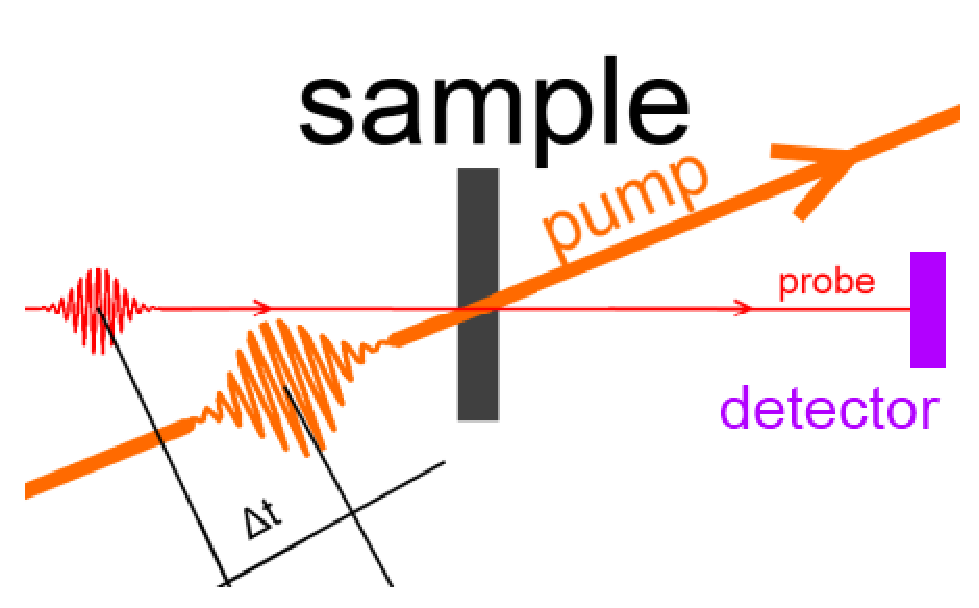
\includegraphics{img/pnp.eps}
{\small 
[Figure 2.3.1] - The pump-and-probe process}





The key assumption in the pump-and-probe process is that separated and
independent probe signal cannot saturate the response of atomic system
alone [2]. The probe signal shall be that weak - it will not cause any
more nonlinear effects in the investigated medium. It is important
that investigated molecule has for both the pump and the probe signal
two different relaxation times: 
\mapleinline{inert}{2d}{T[1];}{%
${T_{1}}$%
} and 
\mapleinline{inert}{2d}{T[2];}{%
${T_{2}}$%
} respectively. A complicated model is defined by H. N. Yum et al.
[16] for the nonlinear susceptibility in case of pump-probe process:





(2.3.1a) 
\mapleinline{inert}{2d}{chi[pp](delta);}{%
${\chi _{\mathit{pp}}}(\delta )$%
} = 
\mapleinline{inert}{2d}{G*n^0*gamma[ba]/(Delta+delta+i*eta);}{%
$\frac {G\,n^{0}\,{\gamma _{\mathit{ba}}}}{\Delta  + \delta  + i
\,\eta }$%
} x [ 
\mapleinline{inert}{2d}{1-Omega[1]^2*(Delta-delta+i*eta)*(delta+2*i*eta)/(Delta-i*eta)/((delt
a+i*teta)*(Delta+delta+i*eta)*(delta-Delta+i*eta)-Omega[1]^2*(delta+i*
eta))/2;}{%
$1 - \frac {{\Omega _{1}}^{2}\,(\Delta  - \delta  + i\,\eta )\,(
\delta  + 2\,i\,\eta )}{(\Delta  - i\,\eta )\,((\delta  + i\,
\mathit{teta})\,(\Delta  + \delta  + i\,\eta )\,(\delta  - \Delta
  + i\,\eta ) - {\Omega _{1}}^{2}\,(\delta  + i\,\eta ))\,2}$%
} ]





where:



\mapleinline{inert}{2d}{Omega[1];}{%
${\Omega _{1}}$%
} = 
\mapleinline{inert}{2d}{Omega[1];}{%
${\Omega _{1}}$%
}(
\mapleinline{inert}{2d}{T[1];}{%
${T_{1}}$%
}), G = G(
\mapleinline{inert}{2d}{T[1];}{%
${T_{1}}$%
}), 
\mapleinline{inert}{2d}{n^0;}{%
$n^{0}$%
} = 
\mapleinline{inert}{2d}{n^0;}{%
$n^{0}$%
}(
\mapleinline{inert}{2d}{T[1];}{%
${T_{1}}$%
}), 
\mapleinline{inert}{2d}{gamma[ba] = gamma[ba](T[1]);}{%
${\gamma _{\mathit{ba}}}={\gamma _{\mathit{ba}}}({T_{1}})$%
}, 
\mapleinline{inert}{2d}{eta = eta(T[1]);}{%
$\eta =\eta ({T_{1}})$%
}



\mapleinline{inert}{2d}{delta;}{%
$\delta $%
} - probe frequency



\mapleinline{inert}{2d}{Delta;}{%
$\Delta $%
} - pump prequency





where particular parameters depend on the complicated derivation with
an usage of quantum-mechanics and classical-mechanics approach. Here
the important thing to concider is that the susceptibility of the
probe depends on the relaxation time of pump signal - which in other
words means that:





\mapleinline{inert}{2d}{chi[pp] = chi[pp];}{%
${\chi _{\mathit{pp}}}={\chi _{\mathit{pp}}}$%
}(
\mapleinline{inert}{2d}{delta;}{%
$\delta $%
}, 
\mapleinline{inert}{2d}{T[1];}{%
${T_{1}}$%
}) and 
\mapleinline{inert}{2d}{T[1] = T[1];}{%
${T_{1}}={T_{1}}$%
}(
\mapleinline{inert}{2d}{Delta;}{%
$\Delta $%
}t)





In sense of the response theory this observation leads us to the
conclusion, that the suscebility of the nonlinear process depends not
only on the input signal frequency (energy) - but also on the time
delay between the moments, when two or more photons shots the
molecule. The literature we have found is in lack of advanced model -
so here we are talking about the cutting edge problem in nonlinear
optics and the constructing of the valid model for the pump-and-probe
process - so the Kramers-Kronig relations should be applied here. We
also deduce from the response theory, that the output signal in the
pump-and-probe process does not shows instantly, but after the last
photon shots the investigated molecule - so we have some type of pause
- which observation should expand the linear response theory.



In [20] we can found results that proofs that the probe signal
absorbance depends not only on the pump signal properties, but also on
the delay time between the pump and probe - see Figure 2.3.2



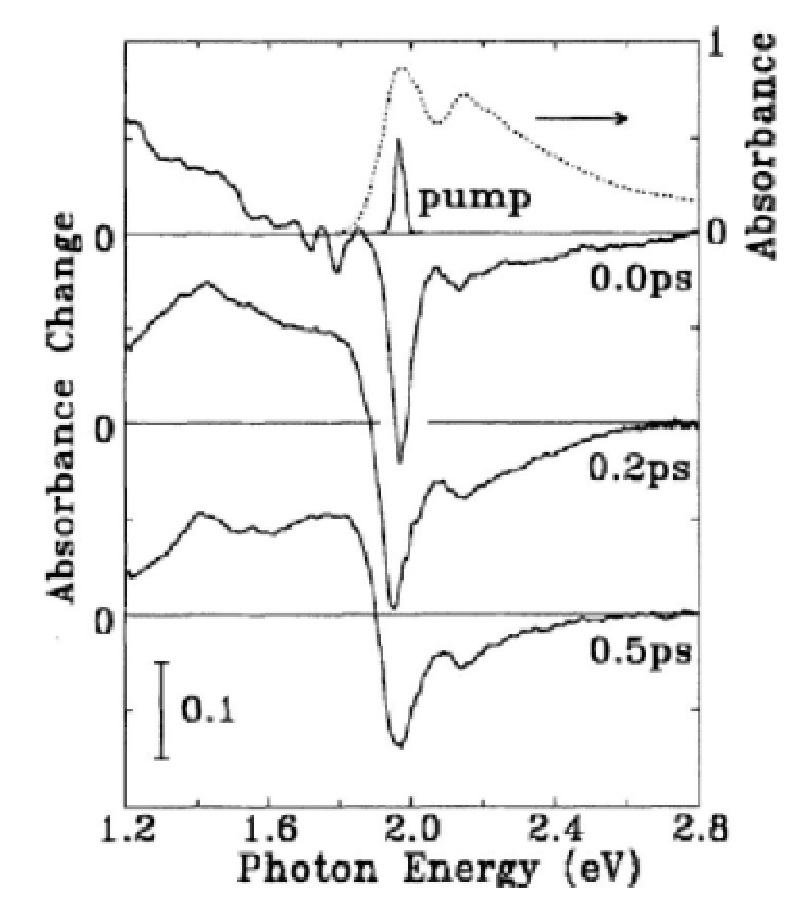
\includegraphics{img/pnp_abs.eps}


{\small [Figure 2.3.2] - The pump-and-probe absorption change dure to
time delay between the pump and probe signal. Figure taken from [20].}





The more interesting results come when we assume, that susceptibility
is a complex function of two parameters, both the pump and probe
signal frequency:





(2.3.1b) 
\mapleinline{inert}{2d}{chi[pp] = chi[pp](delta,Delta);}{%
${\chi _{\mathit{pp}}}={\chi _{\mathit{pp}}}(\delta , \,\Delta )$%
}





Therefore we obtain such an 3-Dimensial plots:





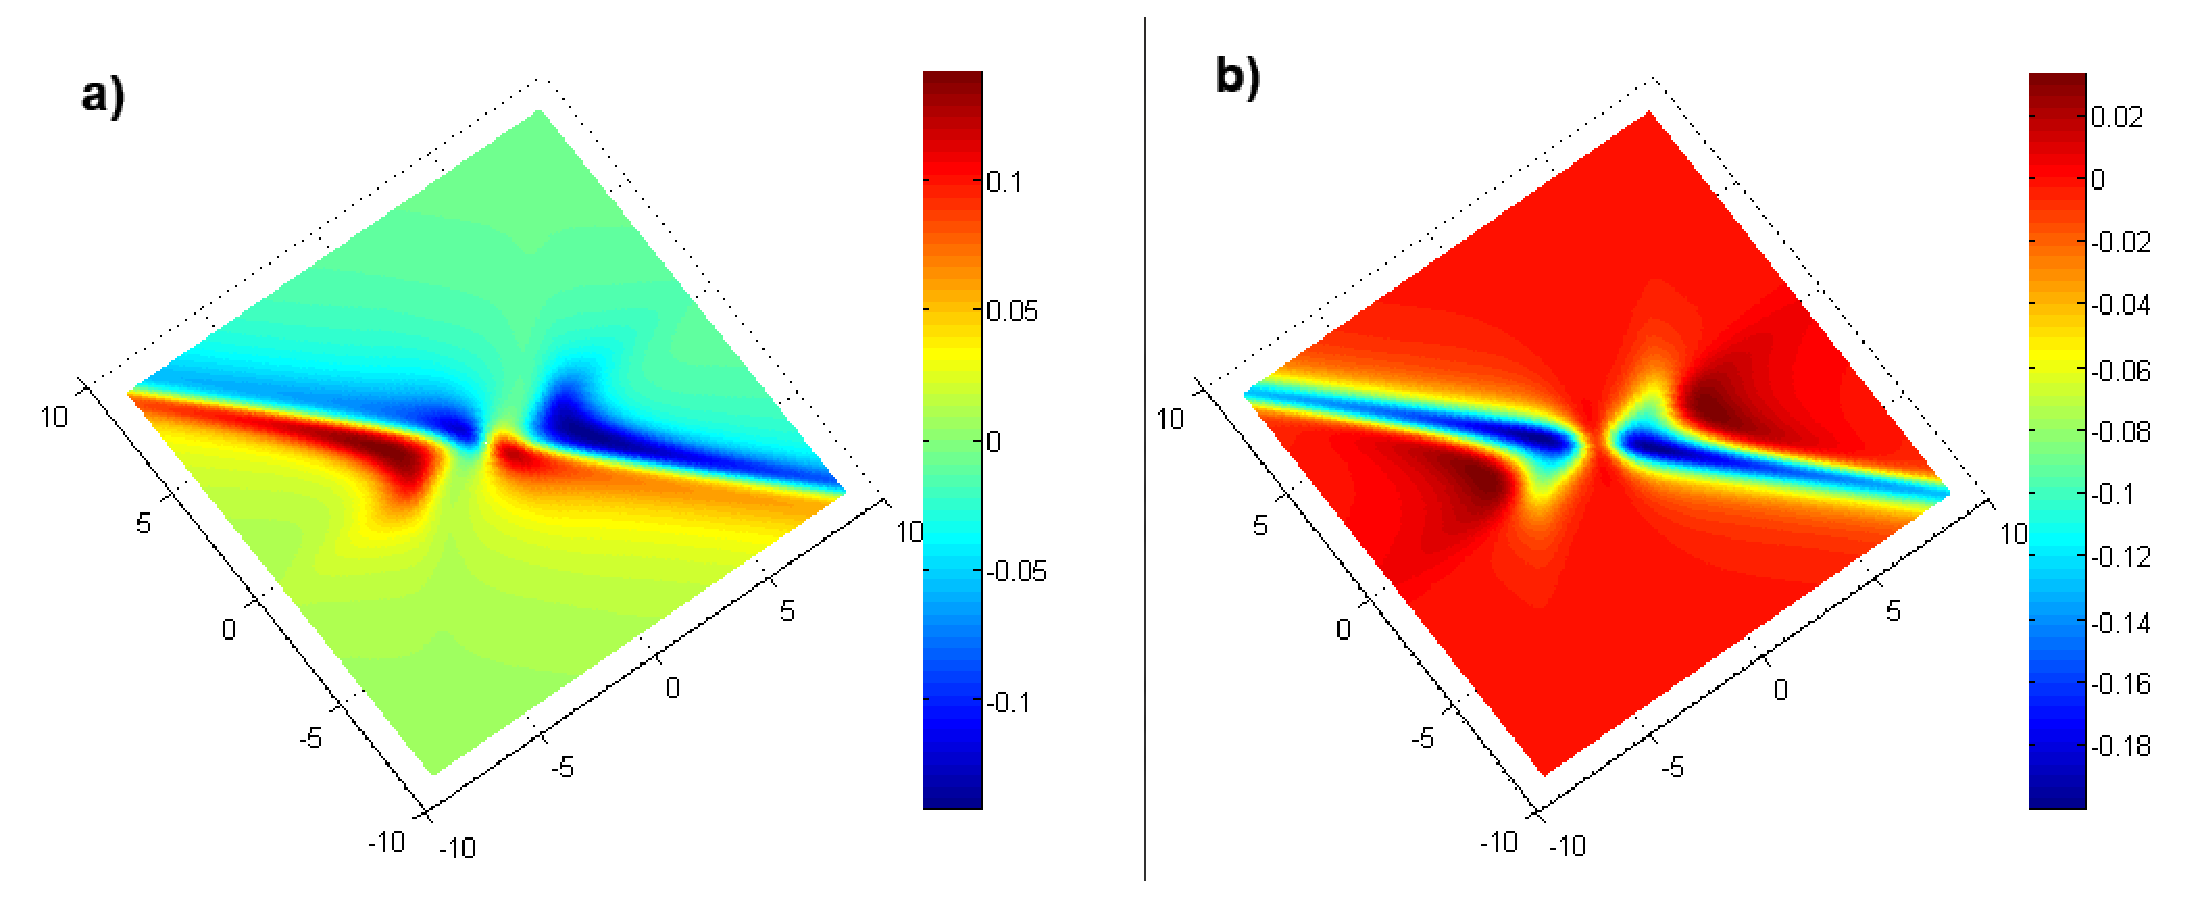
\includegraphics[width=170mm]{img/pnp_2d.eps}
{\small [Figure 2.3.1a, 2.3.1b] 2-Dimensial plots of both a) real and
b) imaginary parts of nonlinear susceptibility threated as a
biargumental function, where the color means the function value}





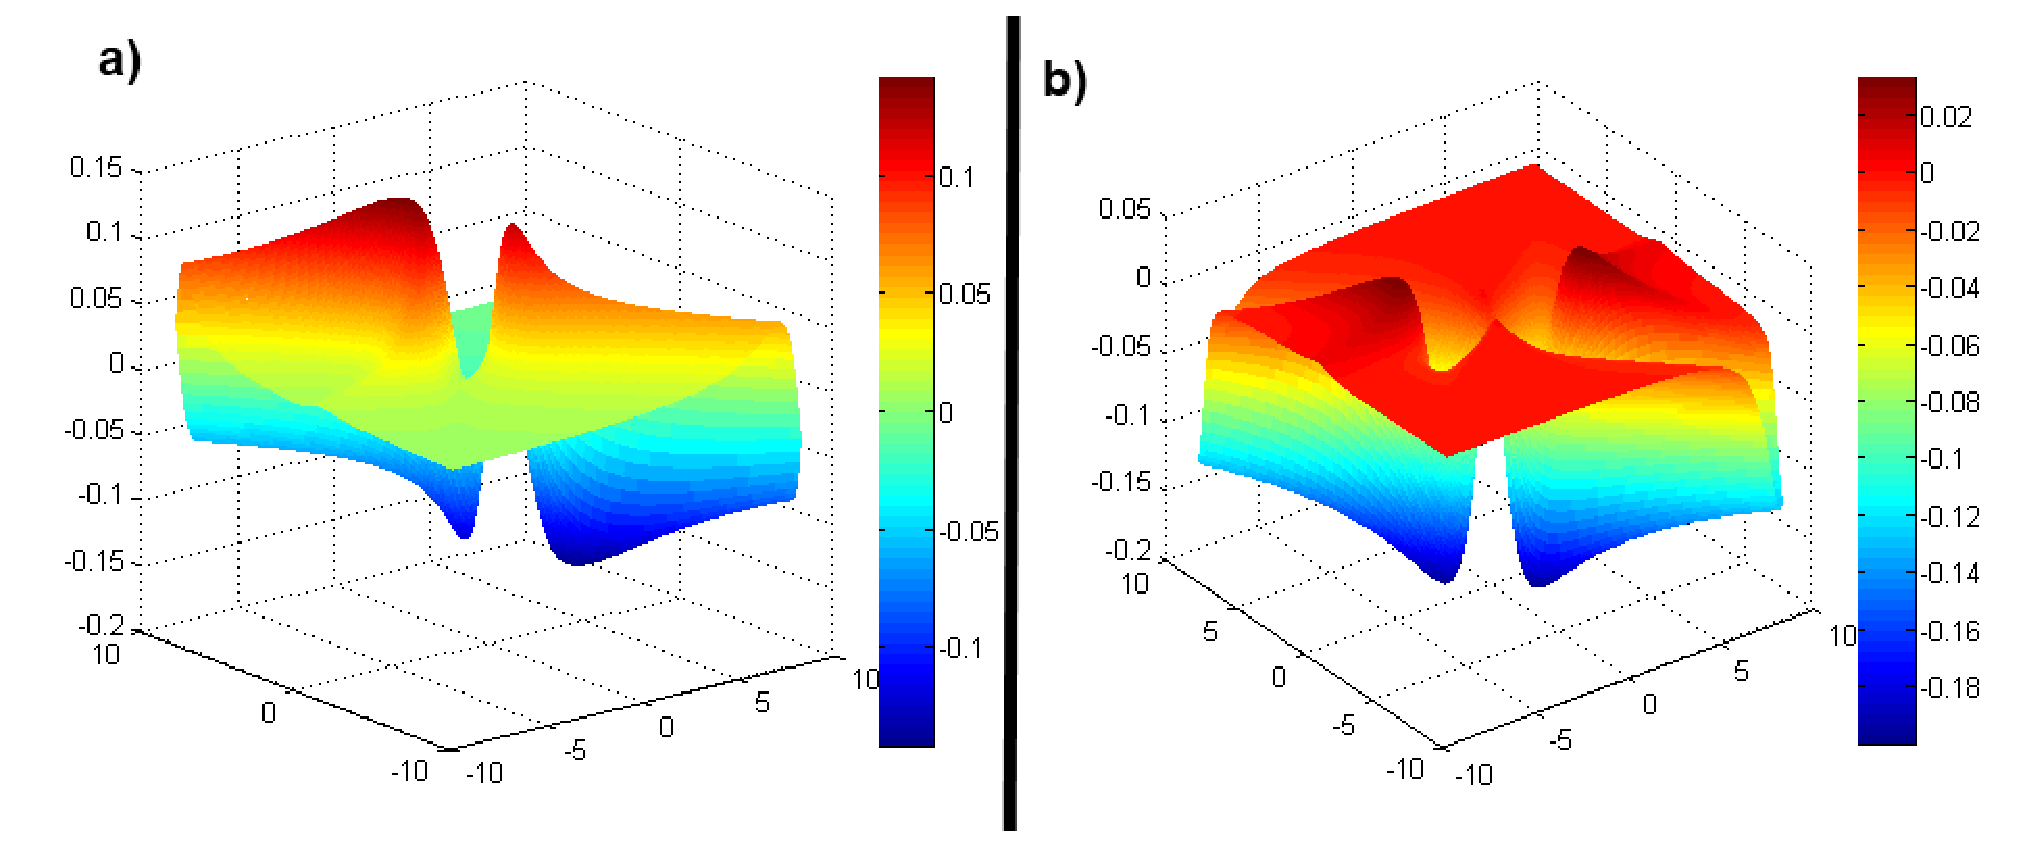
\includegraphics[width=170mm]{img/pnp_3d.eps}
{\small [Figure 2.3.2a, 2.3.2b] 3-Dimensial plots of both a) real and
b) imaginary parts of nonlinear susceptibility threated as a
biargumental function, where the color means the function value}




\subsubsection*{Frequency Mixing Process}



The frequency mixing is a general class of processes when we have two
or more input photons with their frequencies: 
\mapleinline{inert}{2d}{omega[input,1],omega[input,2],omega[input,3];}{%
${\omega _{\mathit{input}, \,1}}, \,{\omega _{\mathit{input}, \,2
}}, \,{\omega _{\mathit{input}, \,3}}$%
}, ... and we receive one or more output photons with their
frequencies: 
\mapleinline{inert}{2d}{omega[output,1],omega[output,2],omega[output,3];}{%
${\omega _{\mathit{output}, \,1}}, \,{\omega _{\mathit{output}, 
\,2}}, \,{\omega _{\mathit{output}, \,3}}$%
}, .... In chapter 6.6 of Boyd [2] we can find the description of
process in which we observe the strong singal 'pump' with frequency 
\mapleinline{inert}{2d}{omega;}{%
$\omega $%
} and the weak signal 'probe' with the frequency 
\mapleinline{inert}{2d}{omega-delta;}{%
$\omega  - \delta $%
} nearly copropragating, as has been shown on the figure [2.3.3]





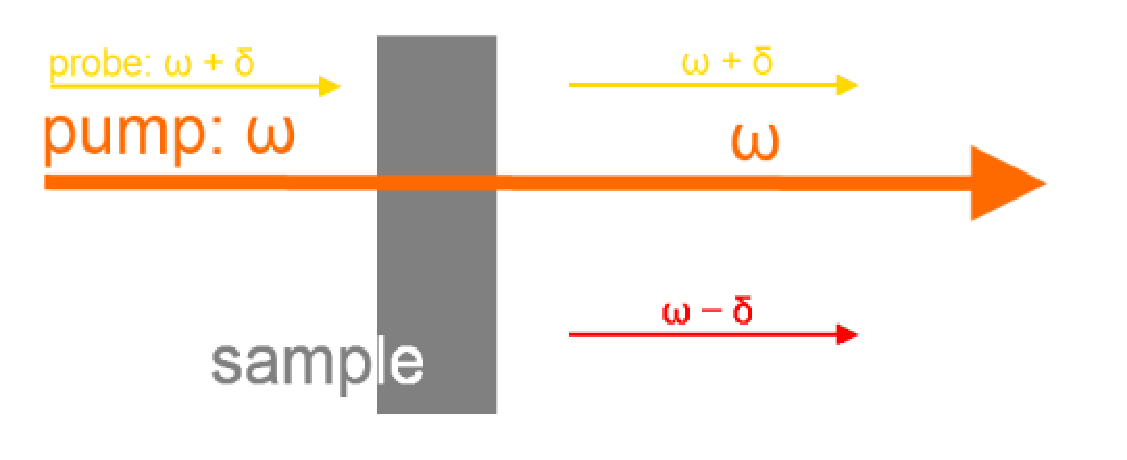
\includegraphics{img/fmix_sch.eps}



{\small [Figure 2.3.3] - The pump-and-probe frequency mixing process
from chapter 6.6 Boyd [2]}





For such process a model for the linear susceptibilities hase defined
by Boyd for both 
\mapleinline{inert}{2d}{omega+delta;}{%
$\omega  + \delta $%
} and 
\mapleinline{inert}{2d}{omega-delta;}{%
$\omega  - \delta $%
} frequencies:





(2.3.2a) 
\mapleinline{inert}{2d}{chi[eff,1](omega+delta);}{%
${\chi _{\mathit{eff}, \,1}}(\omega  + \delta )$%
} =    
\mapleinline{inert}{2d}{N*abs(mu[ba]^2)*w[0]/(epsilon[0]*h*D(delta))*(delta+i/T[1])*(delta-De
lta+i/T[2]-Omega^2/2*delta/(Delta-i/T[2]));}{%
$\frac {N\, \left|  \! \,{\mu _{\mathit{ba}}}^{2}\, \!  \right| 
\,{w_{0}}\,(\delta  + \frac {i}{{T_{1}}})\, \left(  \! \delta  - 
\Delta  + \frac {i}{{T_{2}}} - \frac {\Omega ^{2}\,\delta }{2\,(
\Delta  - \frac {i}{{T_{2}}})} \!  \right) }{{\varepsilon _{0}}\,
h\,\mathrm{D}(\delta )}$%
}



(2.3.2b) 
\mapleinline{inert}{2d}{chi[eff,1](omega-delta);}{%
${\chi _{\mathit{eff}, \,1}}(\omega  - \delta )$%
} =    
\mapleinline{inert}{2d}{N*abs(mu[ba]^2)*w[0]/(epsilon[0]*h*D(delta))*(-delta+i/T[1])*(-delta-
Delta+i/T[2]+Omega^2/2*delta/(Delta-i/T[2]));}{%
$\frac {N\, \left|  \! \,{\mu _{\mathit{ba}}}^{2}\, \!  \right| 
\,{w_{0}}\,( - \delta  + \frac {i}{{T_{1}}})\, \left(  \!  - 
\delta  - \Delta  + \frac {i}{{T_{2}}} + \frac {\Omega ^{2}\,
\delta }{2\,(\Delta  - \frac {i}{{T_{2}}})} \!  \right) }{{
\varepsilon _{0}}\,h\,\mathrm{D}(\delta )}$%
}





Boyd also derives the third-order nonlinear susceptibilities for both 
\mapleinline{inert}{2d}{omega+delta;}{%
$\omega  + \delta $%
} and 
\mapleinline{inert}{2d}{omega-delta;}{%
$\omega  - \delta $%
} frequencies:





(2.3.3a) 
\mapleinline{inert}{2d}{chi[eff,3](omega+delta = omega+omega-(omega-delta));}{%
${\chi _{\mathit{eff}, \,3}}(\omega  + \delta =\omega  + \omega 
 - (\omega  - \delta ))$%
} =    
\mapleinline{inert}{2d}{2*N*w[0]*mu[ba]^4*(-delta-Delta-i/T[2])*(delta+2*i/T[2])/((Delta+i/T[
2])*3*epsilon[0]*h^3*(Delta+delta+i/T[2])*D[c](delta));}{%
$\frac {2\,N\,{w_{0}}\,{\mu _{\mathit{ba}}}^{4}\,( - \delta  - 
\Delta  - \frac {i}{{T_{2}}})\,(\delta  + \frac {2\,i}{{T_{2}}})
}{(\Delta  + \frac {i}{{T_{2}}})\,3\,{\varepsilon _{0}}\,h^{3}\,(
\Delta  + \delta  + \frac {i}{{T_{2}}})\,{\mathrm{D}_{c}}(\delta 
)}$%
}



(2.3.3b) 
\mapleinline{inert}{2d}{chi[eff,3](omega-delta = omega+omega-(omega+delta));}{%
${\chi _{\mathit{eff}, \,3}}(\omega  - \delta =\omega  + \omega 
 - (\omega  + \delta ))$%
} =    
\mapleinline{inert}{2d}{2*N*w[0]*mu[ba]^4*(delta-Delta-i/T[2])*(-delta+2*i/T[2])/((Delta+i/T[
2])*3*epsilon[0]*h^3*(Delta-delta+i/T[2])*D[c](delta));}{%
$\frac {2\,N\,{w_{0}}\,{\mu _{\mathit{ba}}}^{4}\,(\delta  - 
\Delta  - \frac {i}{{T_{2}}})\,( - \delta  + \frac {2\,i}{{T_{2}}
})}{(\Delta  + \frac {i}{{T_{2}}})\,3\,{\varepsilon _{0}}\,h^{3}
\,(\Delta  - \delta  + \frac {i}{{T_{2}}})\,{\mathrm{D}_{c}}(
\delta )}$%
}


\emptyline



where:



\mapleinline{inert}{2d}{Delta;}{%
$\Delta $%
} - detuning of the pump wave



h - dashed Planck constant



N - number density of atoms



\mapleinline{inert}{2d}{T[1],T[2];}{%
${T_{1}}, \,{T_{2}}$%
} - relaxation times



\mapleinline{inert}{2d}{D[c](delta);}{%
${\mathrm{D}_{c}}(\delta )$%
} - conjugate function of D
D - a complex pump-probe function described with (2.3.2c)





(2.3.4c) 
\mapleinline{inert}{2d}{D(delta) =
(delta+1/T[1])*(delta-Delta+i/T[2])*(delta+Delta+i/T[2])-Omega^2*(delt
a+i/T[2]);}{%
$\mathrm{D}(\delta )=(\delta  + \frac {1}{{T_{1}}})\,(\delta  - 
\Delta  + \frac {i}{{T_{2}}})\,(\delta  + \Delta  + \frac {i}{{T
_{2}}}) - \Omega ^{2}\,(\delta  + \frac {i}{{T_{2}}})$%
} 





It is also found [2] that the total response in freqency domain is
stated by the following polarization equations:





(2.3.5a) 
\mapleinline{inert}{2d}{P(omega+delta) =
epsilon[0]*chi[eff,1](omega+delta)*E[1]+3*epsilon[0]*chi[eff,3](w+delt
a = omega+omega-(omega-delta))*E[0]^2*E[-1];}{%
$\mathrm{P}(\omega  + \delta )={\varepsilon _{0}}\,{\chi _{
\mathit{eff}, \,1}}(\omega  + \delta )\,{E_{1}} + 3\,{\varepsilon
 _{0}}\,{\chi _{\mathit{eff}, \,3}}(w + \delta =\omega  + \omega 
 - (\omega  - \delta ))\,{E_{0}}^{2}\,{E_{ - 1}}$%
}*



(2.3.5b) 
\mapleinline{inert}{2d}{P(omega-delta) =
epsilon[0]*chi[eff,1](omega-delta)*E[-1]+3*epsilon[0]*chi[eff,3](w-del
ta = omega+omega-(omega+delta))*E[0]^2*E[1];}{%
$\mathrm{P}(\omega  - \delta )={\varepsilon _{0}}\,{\chi _{
\mathit{eff}, \,1}}(\omega  - \delta )\,{E_{ - 1}} + 3\,{
\varepsilon _{0}}\,{\chi _{\mathit{eff}, \,3}}(w - \delta =\omega
  + \omega  - (\omega  + \delta ))\,{E_{0}}^{2}\,{E_{1}}$%
}*





where:



\mapleinline{inert}{2d}{E[0];}{%
${E_{0}}$%
} - electric field of pump  (with frequency 
\mapleinline{inert}{2d}{omega;}{%
$\omega $%
})



\mapleinline{inert}{2d}{E[1];}{%
${E_{1}}$%
} - electric field of probe (with frequency 
\mapleinline{inert}{2d}{omega+delta;}{%
$\omega  + \delta $%
})



\mapleinline{inert}{2d}{E[-1];}{%
${E_{ - 1}}$%
} - electric field of probe (with frequency 
\mapleinline{inert}{2d}{omega-delta;}{%
$\omega  - \delta $%
})



* - denotes the complex conjugate



\mapleinline{inert}{2d}{epsilon[0];}{%
${\varepsilon _{0}}$%
} - dielectric constant





The test 3-Dimensional plot has been presented on the Figures below:





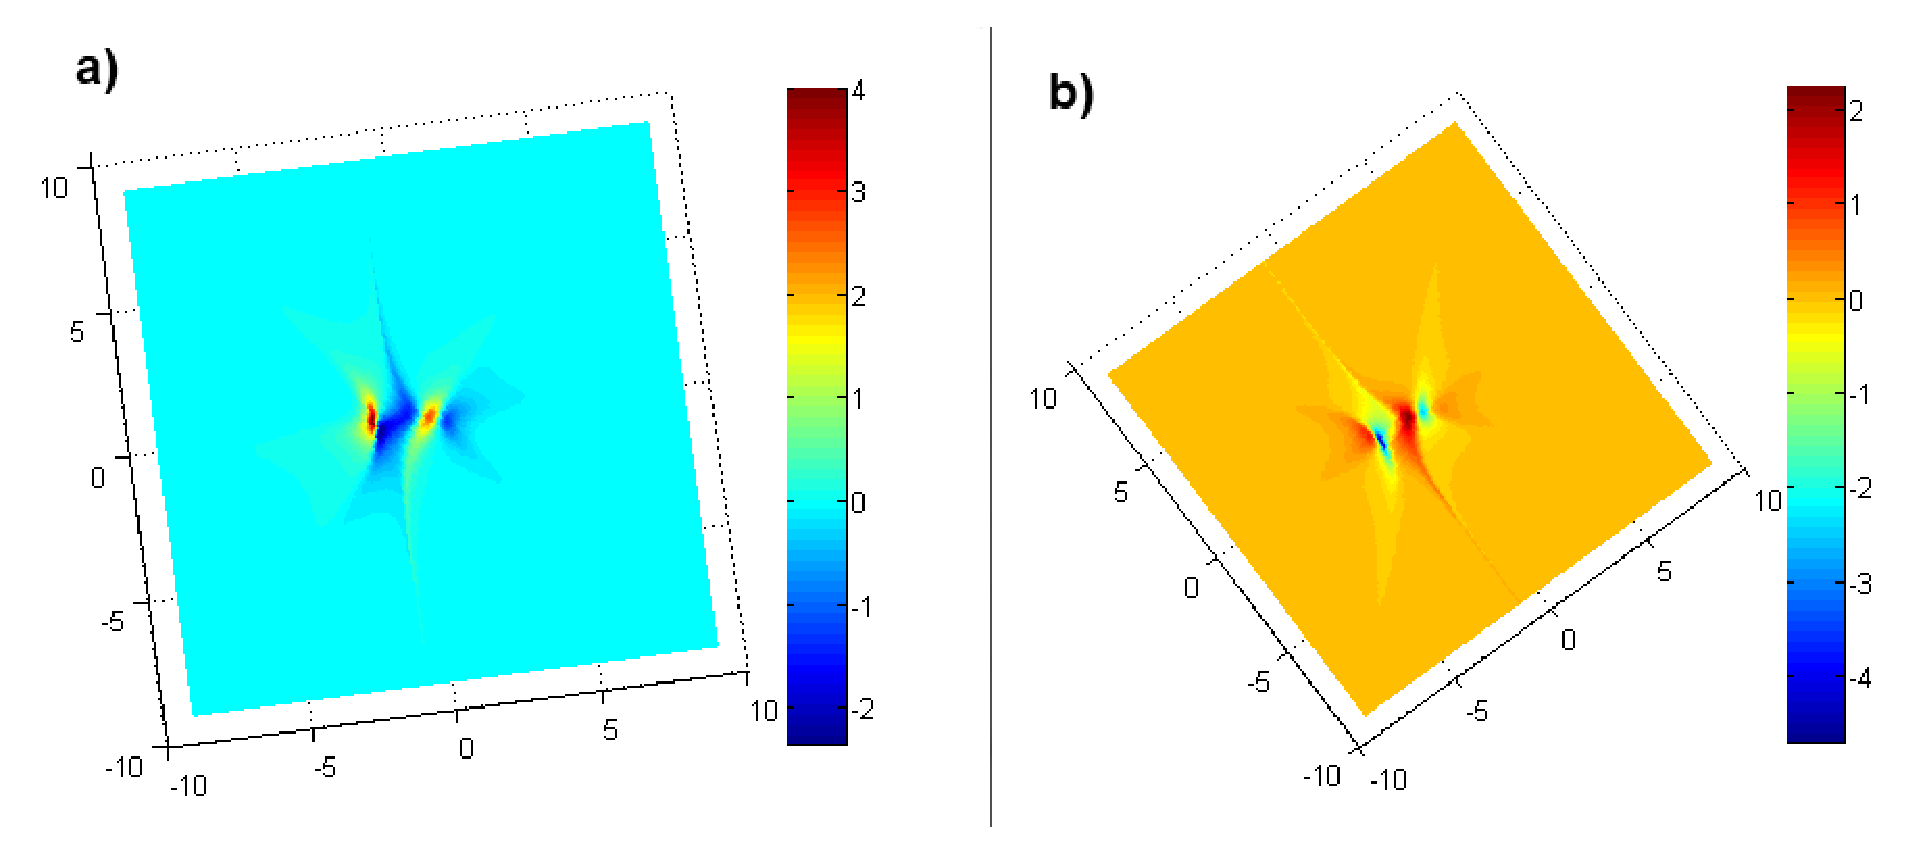
\includegraphics[width=170mm]{img/fmix_2d.eps}

{\small [Figure 2.3.4a-b]  2-Dimensial plots of both a) real and b)
imaginary parts of nonlinear susceptibility threated as a biargumental
function, where the color means the function value}





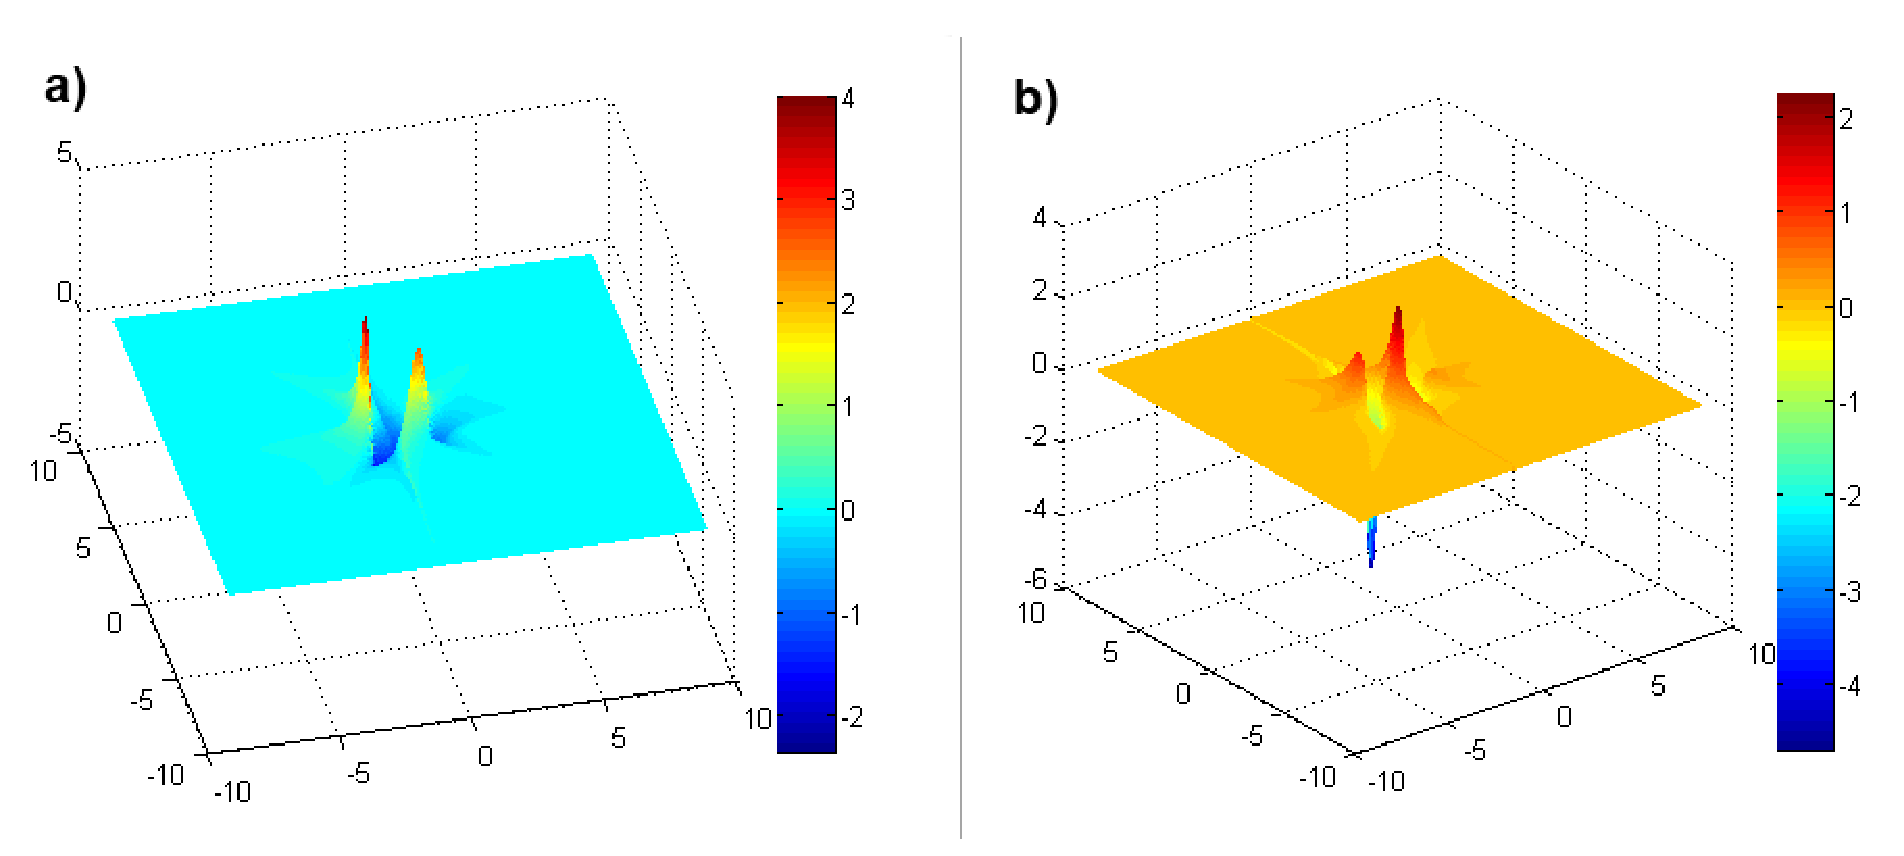
\includegraphics[width=170mm]{img/fmix_3d.eps}

{\small [Figure 2.3.5a-b]  3-Dimensial plots of both a) real and b)
imaginary parts of nonlinear susceptibility threated as a biargumental
function, where the color means the function value}





There are dozens of models for the nonlinear optical phenomena. What
is important in their derivation is to have in mind that the frequency
domain is connected with time domain with the Fourier transform.We
also must remember that to build a valid model - it must obey the
causality principle in the time domain. Here from now we also will
observe that the advanced models of susceptibility does not obey the
rule, that it's real (imaginary) part is an even (odd) function - we
will discuss this in the next chapter.





\textit{Description of simple modification in linear model to obtain
the nonlinear model.}




\subsection{Derivation of the Kramers-Kronig relations for
simple nonlinear model}



As mentioned in equation (2.1.3) in time domain polarization tensor is
calculated using the leading order term of Volterra-series. Now - when
calculating the response of the system under the influence of many
monochromatic light sources - we can formulate the nonlinear multiple
convolution:





(2.4.1) 
\mapleinline{inert}{2d}{P[n,i](t) =
int(int(int(int(G[n,i,j[1],j[2],j[dots],j[n]](t1,t2,tdots,tn)*E[j,1](t
-t[1])*E[j,2](t-t[2])*E[j,dots](t-t[dots])*E[j,n](t-t[n]),t[1]),t[2]),
t[dots]),t[n]);}{%
${P_{n, \,i}}(t)=\int \int \int \int {G_{n, \,i, \,{j_{1}}, \,{j
_{2}}, \,{j_{\mathit{dots}}}, \,{j_{n}}}}(\mathit{t1}, \,\mathit{
t2}, \,\mathit{tdots}, \,\mathit{tn})\,{E_{j, \,1}}(t - {t_{1}})
\,{E_{j, \,2}}(t - {t_{2}})\,{E_{j, \,\mathit{dots}}}(t - {t_{
\mathit{dots}}})\,{E_{j, \,n}}(t - {t_{n}})\,d{t_{1}}\,d{t_{2}}\,
d{t_{\mathit{dots}}}\,d{t_{n}}$%
}





where:



\mapleinline{inert}{2d}{G[n,i,j[1],j[2],j[dots],j[n]](t1,t2,tdots,tn);}{%
${G_{n, \,i, \,{j_{1}}, \,{j_{2}}, \,{j_{\mathit{dots}}}, \,{j_{n
}}}}(\mathit{t1}, \,\mathit{t2}, \,\mathit{tdots}, \,\mathit{tn})
$%
} - the casual n-th order Green function in time domain





After applying the Fourier transform to the (2.4.1) toghether with the
convolution theorem we obtain:





(2.4.2) 
\mapleinline{inert}{2d}{P[n,i](omega) =
int(int(int(int(chi[n,i,j[1],j[2],j[dots],j[n]](sum(omega[l],l = 1 ..
n),omega[1],omega[2],omega[dots],omega[n])*E[j,1](omega[1])*E[j,2](ome
ga[2])*E[j,dots](omega[dots])*E[j,n](omega[n])*delta(omega-sum(omega[l
],l = 1 .. n)),omega[1] = -infinity .. infinity),omega[2] = -infinity
.. infinity),omega[dots] = -infinity .. infinity),omega[n] = -infinity
.. infinity);}{%
${P_{n, \,i}}(\omega )=\int _{ - \infty }^{\infty }\int _{ - 
\infty }^{\infty }\int _{ - \infty }^{\infty }\int _{ - \infty }
^{\infty }{\chi _{n, \,i, \,{j_{1}}, \,{j_{2}}, \,{j_{\mathit{
dots}}}, \,{j_{n}}}}(\sum _{l=1}^{n}\,{\omega _{l}}, \,{\omega _{
1}}, \,{\omega _{2}}, \,{\omega _{\mathit{dots}}}, \,{\omega _{n}
})\,{E_{j, \,1}}({\omega _{1}})\,{E_{j, \,2}}({\omega _{2}})\,{E
_{j, \,\mathit{dots}}}({\omega _{\mathit{dots}}})\,{E_{j, \,n}}({
\omega _{n}})\,\delta (\omega  - (\sum _{l=1}^{n}\,{\omega _{l}})
)\,d{\omega _{1}}\,d{\omega _{2}}\,d{\omega _{\mathit{dots}}}\,d{
\omega _{n}}$%
}





where:



\mapleinline{inert}{2d}{delta;}{%
$\delta $%
} - Dirac delta function





The causality principle can be now assumed for each variable of the
nonlinear Green function in time domain. We therefore can again apply
the Titchmarsh theorem to obtain:





(2.4.3) 
\mapleinline{inert}{2d}{P*int(chi[j,i,j[1],j[2],j[dots],j[n]](sum(Omega[l],l = 1 ..
n),Omega[1],Omega[2],Omega[dots],Omega[n])/(Omega[1]-omega[1]),Omega[1
] = -infinity .. infinity) =
i*pi*chi[n,i,j[1],j[2],j[dots],j[n]](sum(omega[l],l = 1 ..
n),omega[1],omega[2],omega[dots],omega[n]);}{%
$P\,\int _{ - \infty }^{\infty }\frac {{\chi _{j, \,i, \,{j_{1}}
, \,{j_{2}}, \,{j_{\mathit{dots}}}, \,{j_{n}}}}(\sum _{l=1}^{n}\,
{\Omega _{l}}, \,{\Omega _{1}}, \,{\Omega _{2}}, \,{\Omega _{
\mathit{dots}}}, \,{\Omega _{n}})}{{\Omega _{1}} - {\omega _{1}}}
\,d{\Omega _{1}}=i\,\pi \,{\chi _{n, \,i, \,{j_{1}}, \,{j_{2}}, 
\,{j_{\mathit{dots}}}, \,{j_{n}}}}(\sum _{l=1}^{n}\,{\omega _{l}}
, \,{\omega _{1}}, \,{\omega _{2}}, \,{\omega _{\mathit{dots}}}, 
\,{\omega _{n}})$%
}





The equation (2.4.3) was taken from Lucarini [14]. At the moment we
are not sure about the symmetry rule in case of nonlinear optics - so
we propose carefully, more general that in [14]:





(2.4.4a) 
\mapleinline{inert}{2d}{Im(chi[n,i,j[1],j[2],j[dots],j[n]](sum(omega[l],l = 1 ..
n),omega[1],omega[2],omega[dots],omega[n])) =
P/((-Pi)^n)*int(int(int(int(Re(chi[n,i,j[1],j[2],j[dots],j[n]](sum(Ome
ga[l],l = 1 ..
n),Omega[1],Omega[2],Omega[dots],Omega[n]))/(Omega[1]-omega[1])/(Omega
[2]-omega[2])/(Omega[dots]-omega[dots])/(Omega[n]-omega[n]),Omega[1] =
-infinity .. infinity),Omega[2] = -infinity .. infinity),Omega[dots] =
-infinity .. infinity),Omega[n] = -infinity .. infinity);}{%
$\Im ({\chi _{n, \,i, \,{j_{1}}, \,{j_{2}}, \,{j_{\mathit{dots}}}
, \,{j_{n}}}}(\sum _{l=1}^{n}\,{\omega _{l}}, \,{\omega _{1}}, \,
{\omega _{2}}, \,{\omega _{\mathit{dots}}}, \,{\omega _{n}}))=
\frac {P\,\int _{ - \infty }^{\infty }\int _{ - \infty }^{\infty 
}\int _{ - \infty }^{\infty }\int _{ - \infty }^{\infty }\frac {
\Re ({\chi _{n, \,i, \,{j_{1}}, \,{j_{2}}, \,{j_{\mathit{dots}}}
, \,{j_{n}}}}(\sum _{l=1}^{n}\,{\Omega _{l}}, \,{\Omega _{1}}, \,
{\Omega _{2}}, \,{\Omega _{\mathit{dots}}}, \,{\Omega _{n}}))}{({
\Omega _{1}} - {\omega _{1}})\,({\Omega _{2}} - {\omega _{2}})\,(
{\Omega _{\mathit{dots}}} - {\omega _{\mathit{dots}}})\,({\Omega 
_{n}} - {\omega _{n}})}\,d{\Omega _{1}}\,d{\Omega _{2}}\,d{\Omega
 _{\mathit{dots}}}\,d{\Omega _{n}}}{( - \pi )^{n}}$%
}



(2.4.4b) 
\mapleinline{inert}{2d}{Re(chi[n,i,j[1],j[2],j[dots],j[n]](sum(omega[l],l = 1 ..
n),omega[1],omega[2],omega[dots],omega[n])) =
P/(Pi^n)*int(int(int(int(Im(chi[n,i,j[1],j[2],j[dots],j[n]](sum(Omega[
l],l = 1 ..
n),Omega[1],Omega[2],Omega[dots],Omega[n]))/(Omega[1]-omega[1])/(Omega
[2]-omega[2])/(Omega[dots]-omega[dots])/(Omega[n]-omega[n]),Omega[1] =
-infinity .. infinity),Omega[2] = -infinity .. infinity),Omega[dots] =
-infinity .. infinity),Omega[n] = -infinity .. infinity);}{%
$\Re ({\chi _{n, \,i, \,{j_{1}}, \,{j_{2}}, \,{j_{\mathit{dots}}}
, \,{j_{n}}}}(\sum _{l=1}^{n}\,{\omega _{l}}, \,{\omega _{1}}, \,
{\omega _{2}}, \,{\omega _{\mathit{dots}}}, \,{\omega _{n}}))=
\frac {P\,\int _{ - \infty }^{\infty }\int _{ - \infty }^{\infty 
}\int _{ - \infty }^{\infty }\int _{ - \infty }^{\infty }\frac {
\Im ({\chi _{n, \,i, \,{j_{1}}, \,{j_{2}}, \,{j_{\mathit{dots}}}
, \,{j_{n}}}}(\sum _{l=1}^{n}\,{\Omega _{l}}, \,{\Omega _{1}}, \,
{\Omega _{2}}, \,{\Omega _{\mathit{dots}}}, \,{\Omega _{n}}))}{({
\Omega _{1}} - {\omega _{1}})\,({\Omega _{2}} - {\omega _{2}})\,(
{\Omega _{\mathit{dots}}} - {\omega _{\mathit{dots}}})\,({\Omega 
_{n}} - {\omega _{n}})}\,d{\Omega _{1}}\,d{\Omega _{2}}\,d{\Omega
 _{\mathit{dots}}}\,d{\Omega _{n}}}{\pi ^{n}}$%
}





We stress that by the moment we are not sure about the symetry rule
for (2.4.3) because in a typical nonlinear process a response is not
the instant reaction for input - and both the saturation and
reflection processes takes time. When taking into consideration only
one frequency - we conclude that:





(2.4.5a) 
\mapleinline{inert}{2d}{Im(chi[n,i,j[1],j[2],j[dots],j[n]](sum(omega[l],l = 1 ..
n),omega[1],omega[2],omega[dots],omega[n])) =
P/(-Pi)*int(Re(chi[n,i,j[1],j[2],j[dots],j[n]](sum(Omega[l],l = 1 ..
n),Omega[1],Omega[2],Omega[dots],Omega[n]))/(Omega[1]-omega[1]),Omega[
1] = -infinity .. infinity);}{%
$\Im ({\chi _{n, \,i, \,{j_{1}}, \,{j_{2}}, \,{j_{\mathit{dots}}}
, \,{j_{n}}}}(\sum _{l=1}^{n}\,{\omega _{l}}, \,{\omega _{1}}, \,
{\omega _{2}}, \,{\omega _{\mathit{dots}}}, \,{\omega _{n}}))=
\frac {P\,\int _{ - \infty }^{\infty }\frac {\Re ({\chi _{n, \,i
, \,{j_{1}}, \,{j_{2}}, \,{j_{\mathit{dots}}}, \,{j_{n}}}}(\sum 
_{l=1}^{n}\,{\Omega _{l}}, \,{\Omega _{1}}, \,{\Omega _{2}}, \,{
\Omega _{\mathit{dots}}}, \,{\Omega _{n}}))}{{\Omega _{1}} - {
\omega _{1}}}\,d{\Omega _{1}}}{ - \pi }$%
}



(2.4.5b) 
\mapleinline{inert}{2d}{Re(chi[n,i,j[1],j[2],j[dots],j[n]](sum(omega[l],l = 1 ..
n),omega[1],omega[2],omega[dots],omega[n])) =
P/Pi*int(Im(chi[n,i,j[1],j[2],j[dots],j[n]](sum(Omega[l],l = 1 ..
n),Omega[1],Omega[2],Omega[dots],Omega[n]))/(Omega[1]-omega[1]),Omega[
1] = -infinity .. infinity);}{%
$\Re ({\chi _{n, \,i, \,{j_{1}}, \,{j_{2}}, \,{j_{\mathit{dots}}}
, \,{j_{n}}}}(\sum _{l=1}^{n}\,{\omega _{l}}, \,{\omega _{1}}, \,
{\omega _{2}}, \,{\omega _{\mathit{dots}}}, \,{\omega _{n}}))=
\frac {P\,\int _{ - \infty }^{\infty }\frac {\Im ({\chi _{n, \,i
, \,{j_{1}}, \,{j_{2}}, \,{j_{\mathit{dots}}}, \,{j_{n}}}}(\sum 
_{l=1}^{n}\,{\Omega _{l}}, \,{\Omega _{1}}, \,{\Omega _{2}}, \,{
\Omega _{\mathit{dots}}}, \,{\Omega _{n}}))}{{\Omega _{1}} - {
\omega _{1}}}\,d{\Omega _{1}}}{\pi }$%
}





If we focus on the equations (2.4.4a-b) and (2.4.5a-b) it can be seen,
that they lead to the different results. In the latter equations we
are performing only one Hilbert transform for the N-dimensional array
of 
\mapleinline{inert}{2d}{chi[n,i,j[1],j[2],j[dots],j[n]];}{%
${\chi _{n, \,i, \,{j_{1}}, \,{j_{2}}, \,{j_{\mathit{dots}}}, \,{
j_{n}}}}$%
}. In first equation we evalute the Hilbert transform N times and also
the variables are binded within the most innter integrand, so from the
numerical point of view, this multi-integral is harder to evaluate,
because we need to take into consideration the rules of calculating
the multiple-level integral. In further multi-dimensional evaluations
we will use the (2.4.5-ab) equations, because they seem to be valid.
In all equations (2.4.4a-b) and (2.4.5a-b) - we forget about the
symmetry rule despite of the uncertainity howto combine it with the
time-varying saturation and reflection processes. It means that the
signal response does not only depend on the input frequencies 
\mapleinline{inert}{2d}{omega[1],omega[2],omega[dots],omega[n];}{%
${\omega _{1}}, \,{\omega _{2}}, \,{\omega _{\mathit{dots}}}, \,{
\omega _{n}}$%
}, but also on the time delays between them 
\mapleinline{inert}{2d}{T[1],T[2],T[dots],T[n-1];}{%
${T_{1}}, \,{T_{2}}, \,{T_{\mathit{dots}}}, \,{T_{n - 1}}$%
}:





(2.4.6) 
\mapleinline{inert}{2d}{chi[n,i,j[1],j[2],j[dots],j[n]](sum(omega[l],l = 1 ..
n),omega[1],omega[2],omega[dots],omega[n]) =
chi[n,i,j[1],j[2],j[dots],j[n]](sum(omega[l],l = 1 ..
n),omega[1],omega[2],omega[dots],omega[n],T[1],T[2],T[dots],T[N-1]);}{
%
${\chi _{n, \,i, \,{j_{1}}, \,{j_{2}}, \,{j_{\mathit{dots}}}, \,{
j_{n}}}}(\sum _{l=1}^{n}\,{\omega _{l}}, \,{\omega _{1}}, \,{
\omega _{2}}, \,{\omega _{\mathit{dots}}}, \,{\omega _{n}})={\chi
 _{n, \,i, \,{j_{1}}, \,{j_{2}}, \,{j_{\mathit{dots}}}, \,{j_{n}}
}}(\sum _{l=1}^{n}\,{\omega _{l}}, \,{\omega _{1}}, \,{\omega _{2
}}, \,{\omega _{\mathit{dots}}}, \,{\omega _{n}}, \,{T_{1}}, \,{T
_{2}}, \,{T_{\mathit{dots}}}, \,{T_{N - 1}})$%
}





Automatically we expand (2.4.5a-b) into (2.4.7a-b)





(2.4.7a) 
\mapleinline{inert}{2d}{Im(chi[n,i,j[1],j[2],j[dots],j[n]](sum(omega[l],l = 1 ..
n),omega[1],omega[2],omega[dots],omega[n],T[1],T[2],T[dots],T[n-1])) =
P/(-Pi)*int(Re(chi[n,i,j[1],j[2],j[dots],j[n]](sum(Omega[l],l = 1 ..
n),Omega[1],Omega[2],Omega[dots],Omega[n],T[1],T[2],T[dots],T[n-1]))/(
Omega[1]-omega[1]),Omega[1] = -infinity .. infinity);}{%
$\Im ({\chi _{n, \,i, \,{j_{1}}, \,{j_{2}}, \,{j_{\mathit{dots}}}
, \,{j_{n}}}}(\sum _{l=1}^{n}\,{\omega _{l}}, \,{\omega _{1}}, \,
{\omega _{2}}, \,{\omega _{\mathit{dots}}}, \,{\omega _{n}}, \,{T
_{1}}, \,{T_{2}}, \,{T_{\mathit{dots}}}, \,{T_{n - 1}}))=\frac {P
\,\int _{ - \infty }^{\infty }\frac {\Re ({\chi _{n, \,i, \,{j_{1
}}, \,{j_{2}}, \,{j_{\mathit{dots}}}, \,{j_{n}}}}(\sum _{l=1}^{n}
\,{\Omega _{l}}, \,{\Omega _{1}}, \,{\Omega _{2}}, \,{\Omega _{
\mathit{dots}}}, \,{\Omega _{n}}, \,{T_{1}}, \,{T_{2}}, \,{T_{
\mathit{dots}}}, \,{T_{n - 1}}))}{{\Omega _{1}} - {\omega _{1}}}
\,d{\Omega _{1}}}{ - \pi }$%
}



(2.4.7b) 
\mapleinline{inert}{2d}{Re(chi[n,i,j[1],j[2],j[dots],j[n]](sum(omega[l],l = 1 ..
n),omega[1],omega[2],omega[dots],omega[n],T[1],T[2],T[dots],T[N-1])) =
P/Pi*int(Im(chi[n,i,j[1],j[2],j[dots],j[n]](sum(Omega[l],l = 1 ..
n),Omega[1],Omega[2],Omega[dots],Omega[n],T[1],T[2],T[dots],T[n-1]))/(
Omega[1]-omega[1]),Omega[1] = -infinity .. infinity);}{%
$\Re ({\chi _{n, \,i, \,{j_{1}}, \,{j_{2}}, \,{j_{\mathit{dots}}}
, \,{j_{n}}}}(\sum _{l=1}^{n}\,{\omega _{l}}, \,{\omega _{1}}, \,
{\omega _{2}}, \,{\omega _{\mathit{dots}}}, \,{\omega _{n}}, \,{T
_{1}}, \,{T_{2}}, \,{T_{\mathit{dots}}}, \,{T_{N - 1}}))=\frac {P
\,\int _{ - \infty }^{\infty }\frac {\Im ({\chi _{n, \,i, \,{j_{1
}}, \,{j_{2}}, \,{j_{\mathit{dots}}}, \,{j_{n}}}}(\sum _{l=1}^{n}
\,{\Omega _{l}}, \,{\Omega _{1}}, \,{\Omega _{2}}, \,{\Omega _{
\mathit{dots}}}, \,{\Omega _{n}}, \,{T_{1}}, \,{T_{2}}, \,{T_{
\mathit{dots}}}, \,{T_{n - 1}}))}{{\Omega _{1}} - {\omega _{1}}}
\,d{\Omega _{1}}}{\pi }$%
}


\emptyline



One might say that this equations are to general to practically use
them - but for our point of view it is important that in the nonlinear
case we do not need to integrate from zero to plus infinity but
through the full real line - we will keep this assumption in all
further nonlinear calculations.





\textit{Mathematical derivation of the Kramers-Kronig relations for
simple nonlinear model.}




\subsection{Overview of the simple quantum-perturbative model}



We are interested in derivation of the first-order linear
susceptibility and the second-order and third-order nonlinear
susceptibility using the quantum mechanical approach and by solving
the Schr�dinger equation. While this is the cutting edge, most
investigated area of moderd physics and an difficult mathematics area
- we will only try to do the hand-waving introduction into this
matter. What is important in this model, by Boyd [2] that in case of
nonlinear optics the important relaxation process is not taken into
account. As we have written before, the nonlinear susceptibilities
depend not only on the input wave frequency but also on the time
between those impulses - we should try the quantum-perturbative model
as not yet finalized.



The general assumption in the quantum mechanics applied for nonlinear
optics is that the whole material properties can be described using
the time-dependent Schr�dinger equation:





(2.5.1) 
\mapleinline{inert}{2d}{i*h*diff(psi(r,t),t) = H*psi(r,t);}{%
$i\,h\,({\frac {\partial }{\partial t}}\,\psi (r, \,t))=H\,\psi (
r, \,t)$%
}





where:



H - Hamiltonian operator



\mapleinline{inert}{2d}{psi(r,t);}{%
$\psi (r, \,t)$%
} - atomic wavefunction





The H Hamiltonian can be splitted:





(2.5.2) 
\mapleinline{inert}{2d}{H = H[0]+V[t];}{%
$H={H_{0}} + {V_{t}}$%
}





where:
\mapleinline{inert}{2d}{H[0];}{%
${H_{0}}$%
} - Hamiltonian for free atom



\mapleinline{inert}{2d}{V[t];}{%
${V_{t}}$%
} - Hamiltonian for interaction of an atom with electromagnetic field





Hence the (2.5.1) equation is hard to solve exactly, we replace the H
Hamiltonian with:





(2.5.3) 
\mapleinline{inert}{2d}{H = H[0]+lambda*V[t];}{%
$H={H_{0}} + \lambda \,{V_{t}}$%
}





where:



\mapleinline{inert}{2d}{`in`(lambda,C);}{%
$\lambda \,\ \textbf{in}\ \,C$%
}[0,1], perturbative parameter that describes the strength of
interaction





Not jumping into details, we may now try to find a solution to
Schr�dinger�s equation with power the following power series:





(2.5.4) 
\mapleinline{inert}{2d}{psi(r,t) =
psi[0](r,t)+lambda*psi[1](r,t)+lambda^2*psi[2](r,t)+dots;}{%
$\psi (r, \,t)={\psi _{0}}(r, \,t) + \lambda \,{\psi _{1}}(r, \,t
) + \lambda ^{2}\,{\psi _{2}}(r, \,t) + \mathit{dots}$%
}





With such an perturbative assumption we can now modify the initial
(2.5.1) equation into a form:





(2.5.5a) 
\mapleinline{inert}{2d}{i*h*diff(psi[0](r,t),t) = H[0]*psi[0](r,t);}{%
$i\,h\,({\frac {\partial }{\partial t}}\,{\psi _{0}}(r, \,t))={H
_{0}}\,{\psi _{0}}(r, \,t)$%
}



(2.5.5b) 
\mapleinline{inert}{2d}{i*h*diff(psi[n](r,t),t) = H[0]*(psi[n](r,t)+V(t)*psi[n-1](r,t));}{%
$i\,h\,({\frac {\partial }{\partial t}}\,{\psi _{n}}(r, \,t))={H
_{0}}\,({\psi _{n}}(r, \,t) + \mathrm{V}(t)\,{\psi _{n - 1}}(r, 
\,t))$%
}





We call the 
\mapleinline{inert}{2d}{psi[n](r,t);}{%
${\psi _{n}}(r, \,t)$%
} an eigenvector. They can be expanded in terms of unperturbed states
as following:





(2.5.6)  
\mapleinline{inert}{2d}{psi[n](r,t) = sum(a[N,l](t)*u[l](r)*exp(-i*omega[l]*t),l);}{%
${\psi _{n}}(r, \,t)=\sum _{l}\,{a_{N, \,l}}(t)\,{u_{l}}(r)\,e^{(
 - i\,{\omega _{l}}\,t)}$%
}





where:
\mapleinline{inert}{2d}{a[N,l](t);}{%
${a_{N, \,l}}(t)$%
} - amplitude of the probability that the atom is in energy eigenstate
l at time l to the Nth order in perturbation





We next find that:





(2.5.7) 
\mapleinline{inert}{2d}{totaldiff(a[N,l](t)) =
sum(a[N-1,l](t)*V[ml](t)*exp(i*omega[ml]*t),l)/(i*h);}{%
$\mathrm{totaldiff}({a_{N, \,l}}(t))=\frac {\sum _{l}\,{a_{N - 1
, \,l}}(t)\,{V_{\mathit{ml}}}(t)\,e^{(i\,{\omega _{\mathit{ml}}}
\,t)}}{i\,h}$%
}





where:
\mapleinline{inert}{2d}{omega[ml] = omega[m]-omega[l];}{%
${\omega _{\mathit{ml}}}={\omega _{m}} - {\omega _{l}}$%
}
\mapleinline{inert}{2d}{V[ml] = `<|>`(u[m],V(t),u[l]);}{%
${V_{\mathit{ml}}}=\langle {u_{m}}\, | \,\mathrm{V}(t)\, | \,{u_{
l}}\rangle $%
} 





When we integrate (2.5.7) we get:





(2.5.8) 
\mapleinline{inert}{2d}{a[N,l](t) = 1/(h*i);}{%
${a_{N, \,l}}(t)=\frac {1}{h\,i}$%
}
\mapleinline{inert}{2d}{sum(int(V[ml](T)*a[N-1,l](T)*exp(i*omega[ml]*T),T = -infinity ..
t),l);}{%
$\sum _{l}\,\int _{ - \infty }^{t}{V_{\mathit{ml}}}(T)\,{a_{N - 1
, \,l}}(T)\,e^{(i\,{\omega _{\mathit{ml}}}\,T)}\,dT$%
}





From such probability amplitude we will extract the explicit form for
the linear, second-order and third-order optical susceptibilities.
Here we will provide two more physical representations:





(2.5.9a) 
\mapleinline{inert}{2d}{V(t) = -mu*E[x](t);}{%
$\mathrm{V}(t)= - \mu \,{E_{x}}(t)$%
} (
\mapleinline{inert}{2d}{mu;}{%
$\mu $%
} - electric dipole moment operator)
(2.5.9b) 
\mapleinline{inert}{2d}{E[x](t) = sum(E(omega[p])*exp(-i*omega[p]*t),p);}{%
${E_{x}}(t)=\sum _{p}\,\mathrm{E}({\omega _{p}})\,e^{( - i\,{
\omega _{p}}\,t)}$%
} (
\mapleinline{inert}{2d}{E[x](t);}{%
${E_{x}}(t)$%
} - total optical field)





Now it is possible to assume that the linear, second-order and
third-order of the probability amplitude equals:





(2.5.10a) 
\mapleinline{inert}{2d}{a[1,m](t) = 1/h;}{%
${a_{1, \,m}}(t)=\frac {1}{h}$%
}
\mapleinline{inert}{2d}{sum(mu[mg]*E(omega[p])/(omega[mg]-omega[p]),p);}{%
$\sum _{p}\,\frac {{\mu _{\mathit{mg}}}\,\mathrm{E}({\omega _{p}}
)}{{\omega _{\mathit{mg}}} - {\omega _{p}}}$%
}
\mapleinline{inert}{2d}{exp(i*(omega[mg]-omega[p])*t);}{%
$e^{(i\,({\omega _{\mathit{mg}}} - {\omega _{p}})\,t)}$%
}
(2.5.10b) 
\mapleinline{inert}{2d}{a[2,n](t) = 1/(h^2);}{%
${a_{2, \,n}}(t)=\frac {1}{h^{2}}$%
}
\mapleinline{inert}{2d}{sum(sum(mu[nm]*E(omega[q])*mu[mg]*E(omega[p])/(omega[ng]-omega[p]-ome
ga[q])/(omega[mg]-omega[p])/(omega[mg]-omega[p]),m),pq);}{%
$\sum _{\mathit{pq}}\, \left(  \! \sum _{m}\,\frac {{\mu _{
\mathit{nm}}}\,\mathrm{E}({\omega _{q}})\,{\mu _{\mathit{mg}}}\,
\mathrm{E}({\omega _{p}})}{({\omega _{\mathit{ng}}} - {\omega _{p
}} - {\omega _{q}})\,({\omega _{\mathit{mg}}} - {\omega _{p}})\,(
{\omega _{\mathit{mg}}} - {\omega _{p}})} \!  \right) $%
}
\mapleinline{inert}{2d}{exp(i*(omega[mg]-omega[p]-omega[q])*t);}{%
$e^{(i\,({\omega _{\mathit{mg}}} - {\omega _{p}} - {\omega _{q}})
\,t)}$%
}
(2.5.10c) 
\mapleinline{inert}{2d}{a[3,n](t) = 1/(h^3);}{%
${a_{3, \,n}}(t)=\frac {1}{h^{3}}$%
}
\mapleinline{inert}{2d}{sum(sum(mu[vn]*E(omega[r])*mu[nm]*E(omega[q])*mu[mg]*E(omega[p])*1/(o
mega[vg]-omega[p]-omega[q]-omega[r])/(omega[ng]-omega[p]-omega[q])/(om
ega[mg]-omega[p]),mn),pqr);}{%
$\sum _{\mathit{pqr}}\, \left(  \! \sum _{\mathit{mn}}\,\frac {{
\mu _{\mathit{vn}}}\,\mathrm{E}({\omega _{r}})\,{\mu _{\mathit{nm
}}}\,\mathrm{E}({\omega _{q}})\,{\mu _{\mathit{mg}}}\,\mathrm{E}(
{\omega _{p}})\,1}{({\omega _{\mathit{vg}}} - {\omega _{p}} - {
\omega _{q}} - {\omega _{r}})\,({\omega _{\mathit{ng}}} - {\omega
 _{p}} - {\omega _{q}})\,({\omega _{\mathit{mg}}} - {\omega _{p}}
)} \!  \right) $%
}
\mapleinline{inert}{2d}{exp(i*(omega[vg]-omega[p]-omega[q]-omega[r])*t);}{%
$e^{(i\,({\omega _{\mathit{vg}}} - {\omega _{p}} - {\omega _{q}}
 - {\omega _{r}})\,t)}$%
}





respectively. This results will lead us to the following results about
the optical susceptibilities:





(2.5.11a) 
\mapleinline{inert}{2d}{chi[1,i,j](omega[p]) = N/epsilon[0]/h;}{%
${\chi _{1, \,i, \,j}}({\omega _{p}})=\frac {N}{{\varepsilon _{0}
}\,h}$%
}
\mapleinline{inert}{2d}{sum(mu[i,gm]*mu[j,mg]/(omega[mg]-omega[p])+mu[j,gm]*mu[i,mg]/(omega[m
g]+omega[p]),m);}{%
$\sum _{m}\,(\frac {{\mu _{i, \,\mathit{gm}}}\,{\mu _{j, \,
\mathit{mg}}}}{{\omega _{\mathit{mg}}} - {\omega _{p}}} + \frac {
{\mu _{j, \,\mathit{gm}}}\,{\mu _{i, \,\mathit{mg}}}}{{\omega _{
\mathit{mg}}} + {\omega _{p}}})$%
}
(2.5.11b) 
\mapleinline{inert}{2d}{chi[2,i,j,k](omega[p]+omega[q],omega[q],omega[p]) =
N/epsilon[0]/(h^2);}{%
${\chi _{2, \,i, \,j, \,k}}({\omega _{p}} + {\omega _{q}}, \,{
\omega _{q}}, \,{\omega _{p}})=\frac {N}{{\varepsilon _{0}}\,h^{2
}}$%
}
\mapleinline{inert}{2d}{P[I]*sum(mu[i,gn]*mu[j,nm]*mu[k,mg]/(omega[ng]-omega[p]-omega[q])/(om
ega[mg]-omega[p])+mu[j,gn]*mu[i,nm]*mu[k,mg]/(omega[ng]+omega[q])/(ome
ga[mg]-omega[p])+mu[i,gn]*mu[k,nm]*mu[i,mg]/(omega[ng]+omega[q])/(omeg
a[mg]+omega[p]+omega[q]),mn);}{%
${P_{I}}\, \left(  \! \sum _{\mathit{mn}}\,(\frac {{\mu _{i, \,
\mathit{gn}}}\,{\mu _{j, \,\mathit{nm}}}\,{\mu _{k, \,\mathit{mg}
}}}{({\omega _{\mathit{ng}}} - {\omega _{p}} - {\omega _{q}})\,({
\omega _{\mathit{mg}}} - {\omega _{p}})} + \frac {{\mu _{j, \,
\mathit{gn}}}\,{\mu _{i, \,\mathit{nm}}}\,{\mu _{k, \,\mathit{mg}
}}}{({\omega _{\mathit{ng}}} + {\omega _{q}})\,({\omega _{
\mathit{mg}}} - {\omega _{p}})} + \frac {{\mu _{i, \,\mathit{gn}}
}\,{\mu _{k, \,\mathit{nm}}}\,{\mu _{i, \,\mathit{mg}}}}{({\omega
 _{\mathit{ng}}} + {\omega _{q}})\,({\omega _{\mathit{mg}}} + {
\omega _{p}} + {\omega _{q}})}) \!  \right) $%
} where 
\mapleinline{inert}{2d}{P[I];}{%
${P_{I}}$%
} denotes the intrinsic permutation operator
(2.5.11c) 
\mapleinline{inert}{2d}{chi[3,k,j,i,h](omega[sigma],omega[r],omega[q],omega[p]) =
N/epsilon[0]/(h^3);}{%
${\chi _{3, \,k, \,j, \,i, \,h}}({\omega _{\sigma }}, \,{\omega 
_{r}}, \,{\omega _{q}}, \,{\omega _{p}})=\frac {N}{{\varepsilon 
_{0}}\,h^{3}}$%
}
\mapleinline{inert}{2d}{P[I]*sum(mu[k,gv]*mu[j,vn]*mu[i,nm]*mu[h,mg]/((omega[vg]-omega[r]-ome
ga[q]-omega[p])*(omega[ng]-omega[q]-omega[p])*(omega[mg]-omega[p]))+mu
[j,gv]*mu[k,vn]*mu[i,nm]*mu[h,mg]*1/(omega[vg]+omega[r])/(omega[ng]-om
ega[q]-omega[p])/(omega[mg]-omega[p])+mu[j,gv]*mu[i,vn]*mu[k,nm]*mu[h,
mg]*1/(omega[vg]+omega[r])/(omega[ng]+omega[r]+omega[q])/(omega[mg]-om
ega[p])+mu[j,gv]*mu[i,vn]*mu[h,nm]*mu[k,mg]/(omega[vg]+omega[r])/(omeg
a[ng]+omega[r]+omega[q])/(omega[mg]+omega[r]+omega[q]+omega[p]),mnv);}
{%
${P_{I}}\, \left(  \! \sum _{\mathit{mnv}}\,(\frac {{\mu _{k, \,
\mathit{gv}}}\,{\mu _{j, \,\mathit{vn}}}\,{\mu _{i, \,\mathit{nm}
}}\,{\mu _{h, \,\mathit{mg}}}}{({\omega _{\mathit{vg}}} - {\omega
 _{r}} - {\omega _{q}} - {\omega _{p}})\,({\omega _{\mathit{ng}}}
 - {\omega _{q}} - {\omega _{p}})\,({\omega _{\mathit{mg}}} - {
\omega _{p}})} + \frac {{\mu _{j, \,\mathit{gv}}}\,{\mu _{k, \,
\mathit{vn}}}\,{\mu _{i, \,\mathit{nm}}}\,{\mu _{h, \,\mathit{mg}
}}\,1}{({\omega _{\mathit{vg}}} + {\omega _{r}})\,({\omega _{
\mathit{ng}}} - {\omega _{q}} - {\omega _{p}})\,({\omega _{
\mathit{mg}}} - {\omega _{p}})} + \frac {{\mu _{j, \,\mathit{gv}}
}\,{\mu _{i, \,\mathit{vn}}}\,{\mu _{k, \,\mathit{nm}}}\,{\mu _{h
, \,\mathit{mg}}}\,1}{({\omega _{\mathit{vg}}} + {\omega _{r}})\,
({\omega _{\mathit{ng}}} + {\omega _{r}} + {\omega _{q}})\,({
\omega _{\mathit{mg}}} - {\omega _{p}})} + \frac {{\mu _{j, \,
\mathit{gv}}}\,{\mu _{i, \,\mathit{vn}}}\,{\mu _{h, \,\mathit{nm}
}}\,{\mu _{k, \,\mathit{mg}}}}{({\omega _{\mathit{vg}}} + {\omega
 _{r}})\,({\omega _{\mathit{ng}}} + {\omega _{r}} + {\omega _{q}}
)\,({\omega _{\mathit{mg}}} + {\omega _{r}} + {\omega _{q}} + {
\omega _{p}})}) \!  \right) $%
}





Derivation and euqation details may be found in Kuzyk [21] and Boyd
[2]. The (2.5.11b-c) equations are sometimes called the
sum-over-states euqations, becaouse we are performing the sum over all
possible excited states of the atom. Using the another physical model
- called the density matrix operator, we can obtain another set of
equations which are a slight modifications of (2.5.11a-c):





(2.5.12a) 
\mapleinline{inert}{2d}{chi[1](omega[p]) = N/epsilon[0]/h;}{%
${\chi _{1}}({\omega _{p}})=\frac {N}{{\varepsilon _{0}}\,h}$%
}
\mapleinline{inert}{2d}{sum(mu[i,an]*mu[j,na]/(omega[na]-omega[p]-i*gamma[na])+mu[i,na]*mu[j,
an]/(omega[na]-omega[p]+i*gamma[na]),n);}{%
$\sum _{n}\,(\frac {{\mu _{i, \,\mathit{an}}}\,{\mu _{j, \,
\mathit{na}}}}{{\omega _{\mathit{na}}} - {\omega _{p}} - i\,{
\gamma _{\mathit{na}}}} + \frac {{\mu _{i, \,\mathit{na}}}\,{\mu 
_{j, \,\mathit{an}}}}{{\omega _{\mathit{na}}} - {\omega _{p}} + i
\,{\gamma _{\mathit{na}}}})$%
}
(2.5.12b) 
\mapleinline{inert}{2d}{chi[2,i,j,k](omega[p]+omega[q],omega[q],omega[p]) =
N/2/epsilon[0]/(h^2);}{%
${\chi _{2, \,i, \,j, \,k}}({\omega _{p}} + {\omega _{q}}, \,{
\omega _{q}}, \,{\omega _{p}})=\frac {N}{2\,{\varepsilon _{0}}\,h
^{2}}$%
}
\mapleinline{inert}{2d}{sum(rho[0,ll]*(mu[i,l,n]*mu[j,nm]*mu[k,ml]/(omega[nl]-omega[p]-omega[
q]-i*gamma[nl])/(omega[ml]-omega[p]-i*gamma[ml])+mu[i,l,n]*mu[k,nm]*mu
[j,ml]/(omega[nl]-omega[p]-omega[p]-i*gamma[nl])/(omega[ml]-omega[q]-i
*gamma[ml])+mu[k,l,n]*mu[i,nm]*mu[j,ml]/(omega[mn]-omega[p]-omega[q]-i
*gamma[mn])/(omega[nl]+omega[q]+i*gamma[nl])+mu[j,l,n]*mu[i,nm]*mu[k,m
l]/(omega[mn]-omega[p]-omega[q]-i*gamma[mn])/(omega[nl]+omega[q]+i*gam
ma[nl])+mu[j,l,n]*mu[i,nm]*mu[k,ml]/(omega[nm]+omega[p]+omega[q]+i*gam
ma[nm])/(omega[ml]-omega[p]-i*gamma[ml])+mu[k,l,n]*mu[j,nm]*mu[i,ml]/(
omega[nm]+omega[p]+omega[q]+i*gamma[nm])/(omega[ml]-omega[p]-i*gamma[m
l])+mu[k,l,n]*mu[j,nm]*mu[i,ml]/(omega[ml]+omega[p]+omega[q]+i*gamma[m
l])/(omega[nl]+omega[p]+i*gamma[nl])+mu[j,l,n]*mu[k,nm]*mu[i,ml]/(omeg
a[ml]+omega[p]+omega[q]+i*gamma[ml])/(omega[nl]+omega[q]+i*gamma[nl]))
,lmn);}{%
$\sum _{\mathit{lmn}}\,{\rho _{0, \,\mathit{ll}}}\,(\frac {{\mu 
_{i, \,l, \,n}}\,{\mu _{j, \,\mathit{nm}}}\,{\mu _{k, \,\mathit{
ml}}}}{({\omega _{\mathit{nl}}} - {\omega _{p}} - {\omega _{q}}
 - i\,{\gamma _{\mathit{nl}}})\,({\omega _{\mathit{ml}}} - {
\omega _{p}} - i\,{\gamma _{\mathit{ml}}})} + \frac {{\mu _{i, \,
l, \,n}}\,{\mu _{k, \,\mathit{nm}}}\,{\mu _{j, \,\mathit{ml}}}}{(
{\omega _{\mathit{nl}}} - {\omega _{p}} - {\omega _{p}} - i\,{
\gamma _{\mathit{nl}}})\,({\omega _{\mathit{ml}}} - {\omega _{q}}
 - i\,{\gamma _{\mathit{ml}}})} + \frac {{\mu _{k, \,l, \,n}}\,{
\mu _{i, \,\mathit{nm}}}\,{\mu _{j, \,\mathit{ml}}}}{({\omega _{
\mathit{mn}}} - {\omega _{p}} - {\omega _{q}} - i\,{\gamma _{
\mathit{mn}}})\,({\omega _{\mathit{nl}}} + {\omega _{q}} + i\,{
\gamma _{\mathit{nl}}})} + \frac {{\mu _{j, \,l, \,n}}\,{\mu _{i
, \,\mathit{nm}}}\,{\mu _{k, \,\mathit{ml}}}}{({\omega _{\mathit{
mn}}} - {\omega _{p}} - {\omega _{q}} - i\,{\gamma _{\mathit{mn}}
})\,({\omega _{\mathit{nl}}} + {\omega _{q}} + i\,{\gamma _{
\mathit{nl}}})} + \frac {{\mu _{j, \,l, \,n}}\,{\mu _{i, \,
\mathit{nm}}}\,{\mu _{k, \,\mathit{ml}}}}{({\omega _{\mathit{nm}}
} + {\omega _{p}} + {\omega _{q}} + i\,{\gamma _{\mathit{nm}}})\,
({\omega _{\mathit{ml}}} - {\omega _{p}} - i\,{\gamma _{\mathit{
ml}}})} + \frac {{\mu _{k, \,l, \,n}}\,{\mu _{j, \,\mathit{nm}}}
\,{\mu _{i, \,\mathit{ml}}}}{({\omega _{\mathit{nm}}} + {\omega 
_{p}} + {\omega _{q}} + i\,{\gamma _{\mathit{nm}}})\,({\omega _{
\mathit{ml}}} - {\omega _{p}} - i\,{\gamma _{\mathit{ml}}})} + 
\frac {{\mu _{k, \,l, \,n}}\,{\mu _{j, \,\mathit{nm}}}\,{\mu _{i
, \,\mathit{ml}}}}{({\omega _{\mathit{ml}}} + {\omega _{p}} + {
\omega _{q}} + i\,{\gamma _{\mathit{ml}}})\,({\omega _{\mathit{nl
}}} + {\omega _{p}} + i\,{\gamma _{\mathit{nl}}})} + \frac {{\mu 
_{j, \,l, \,n}}\,{\mu _{k, \,\mathit{nm}}}\,{\mu _{i, \,\mathit{
ml}}}}{({\omega _{\mathit{ml}}} + {\omega _{p}} + {\omega _{q}}
 + i\,{\gamma _{\mathit{ml}}})\,({\omega _{\mathit{nl}}} + {
\omega _{q}} + i\,{\gamma _{\mathit{nl}}})})$%
}
(2.5.12c) 
\mapleinline{inert}{2d}{chi[3,k,j,i,h](omega[p]+omega[q]+omega[r],omega[r],omega[q],omega[p])
= N/epsilon[0]/(h^3);}{%
${\chi _{3, \,k, \,j, \,i, \,h}}({\omega _{p}} + {\omega _{q}} + 
{\omega _{r}}, \,{\omega _{r}}, \,{\omega _{q}}, \,{\omega _{p}})
=\frac {N}{{\varepsilon _{0}}\,h^{3}}$%
}
\mapleinline{inert}{2d}{sum(rho[0,ll]*(mu[k,lv]*mu[j,vn]*mu[i,nm]*mu[h,ml]/(omega[vl]-omega[p
]-omega[q]-omega[r]-i*gamma[vl])/(omega[nl]-omega[p]-omega[q]-i*gamma[
nl])/(omega[ml]-omega[p]-i*gamma[ml])+mu[h,lv]*mu[k,vn]*mu[j,nm]*mu[i,
ml]/(omega[nv]-omega[p]-omega[q]-omega[r]-i*nv)/(omega[mv]-omega[p]-om
ega[q]-i*gamma[mv])/(omega[vl]+omega[p]+i*gamma[vl])+mu[i,lv]*mu[k,vn]
*mu[j,nm]*mu[h,ml]/(omega[nv]-omega[p]-omega[q]-omega[r]-i*gamma[nv])/
(omega[vm]+omega[p]+omega[q]+i*gamma[vm])*(omega[ml]-omega[p]-i*gamma[
ml])+mu[h,lv]*mu[i,vn]*mu[k,nm]*mu[j,ml]/(omega[mn]-omega[p]-omega[q]-
omega[r]-i*gamma[mn])/(omega[nl]-omega[p]-omega[q]+i*gamma[nl])/(omega
[vl]+omega[p]+i*gamma[vl])+mu[j,lv]*mu[k,vn]*mu[i,nm]*mu[h,ml]/(omega[
vn]-omega[p]-omega[q]-omega[r]+i*gamma[vn])/(omega[nl]-omega[p]-omega[
q]-i*gamma[nl])/(omega[ml]-omega[p]-i*gamma[ml])+mu[h,lv]*mu[j,vn]*mu[
k,nm]*mu[i,ml]/(omega[nm]+omega[p]+omega[q]+omega[r]+i*gamma[nm])/(ome
ga[mv]-omega[p]-omega[q]-i*gamma[mv])/(omega[vl]+omega[p]+i*gamma[vl])
+omega[i,lv]*mu[j,vn]*mu[k,nm]*mu[h,ml]/(omega[vm]+omega[p]+omega[q]+o
mega[r]+i*gamma[nm])/(omega[vm]+omega[p]+omega[q]+i*gamma[mv])/(omega[
ml]-omega[p]-i*gamma[ml])+mu[h,lv]*mu[i,vn]*mu[j,mn]*mu[k,ml]/(omega[m
l]+omega[p]+omega[q]+omega[r]+i*gamma[ml])/(omega[nl]+omega[p]+omega[q
]+i*gamma[nl])/(omega[vl]+omega[p]+i*gamma[vl])),vnml);}{%
$\sum _{\mathit{vnml}}\,{\rho _{0, \,\mathit{ll}}}\,(\frac {{\mu 
_{k, \,\mathit{lv}}}\,{\mu _{j, \,\mathit{vn}}}\,{\mu _{i, \,
\mathit{nm}}}\,{\mu _{h, \,\mathit{ml}}}}{({\omega _{\mathit{vl}}
} - {\omega _{p}} - {\omega _{q}} - {\omega _{r}} - i\,{\gamma _{
\mathit{vl}}})\,({\omega _{\mathit{nl}}} - {\omega _{p}} - {
\omega _{q}} - i\,{\gamma _{\mathit{nl}}})\,({\omega _{\mathit{ml
}}} - {\omega _{p}} - i\,{\gamma _{\mathit{ml}}})} + \frac {{\mu 
_{h, \,\mathit{lv}}}\,{\mu _{k, \,\mathit{vn}}}\,{\mu _{j, \,
\mathit{nm}}}\,{\mu _{i, \,\mathit{ml}}}}{({\omega _{\mathit{nv}}
} - {\omega _{p}} - {\omega _{q}} - {\omega _{r}} - i\,\mathit{nv
})\,({\omega _{\mathit{mv}}} - {\omega _{p}} - {\omega _{q}} - i
\,{\gamma _{\mathit{mv}}})\,({\omega _{\mathit{vl}}} + {\omega _{
p}} + i\,{\gamma _{\mathit{vl}}})} + \frac {{\mu _{i, \,\mathit{
lv}}}\,{\mu _{k, \,\mathit{vn}}}\,{\mu _{j, \,\mathit{nm}}}\,{\mu
 _{h, \,\mathit{ml}}}\,({\omega _{\mathit{ml}}} - {\omega _{p}}
 - i\,{\gamma _{\mathit{ml}}})}{({\omega _{\mathit{nv}}} - {
\omega _{p}} - {\omega _{q}} - {\omega _{r}} - i\,{\gamma _{
\mathit{nv}}})\,({\omega _{\mathit{vm}}} + {\omega _{p}} + {
\omega _{q}} + i\,{\gamma _{\mathit{vm}}})} + \frac {{\mu _{h, \,
\mathit{lv}}}\,{\mu _{i, \,\mathit{vn}}}\,{\mu _{k, \,\mathit{nm}
}}\,{\mu _{j, \,\mathit{ml}}}}{({\omega _{\mathit{mn}}} - {\omega
 _{p}} - {\omega _{q}} - {\omega _{r}} - i\,{\gamma _{\mathit{mn}
}})\,({\omega _{\mathit{nl}}} - {\omega _{p}} - {\omega _{q}} + i
\,{\gamma _{\mathit{nl}}})\,({\omega _{\mathit{vl}}} + {\omega _{
p}} + i\,{\gamma _{\mathit{vl}}})} + \frac {{\mu _{j, \,\mathit{
lv}}}\,{\mu _{k, \,\mathit{vn}}}\,{\mu _{i, \,\mathit{nm}}}\,{\mu
 _{h, \,\mathit{ml}}}}{({\omega _{\mathit{vn}}} - {\omega _{p}}
 - {\omega _{q}} - {\omega _{r}} + i\,{\gamma _{\mathit{vn}}})\,(
{\omega _{\mathit{nl}}} - {\omega _{p}} - {\omega _{q}} - i\,{
\gamma _{\mathit{nl}}})\,({\omega _{\mathit{ml}}} - {\omega _{p}}
 - i\,{\gamma _{\mathit{ml}}})} + \frac {{\mu _{h, \,\mathit{lv}}
}\,{\mu _{j, \,\mathit{vn}}}\,{\mu _{k, \,\mathit{nm}}}\,{\mu _{i
, \,\mathit{ml}}}}{({\omega _{\mathit{nm}}} + {\omega _{p}} + {
\omega _{q}} + {\omega _{r}} + i\,{\gamma _{\mathit{nm}}})\,({
\omega _{\mathit{mv}}} - {\omega _{p}} - {\omega _{q}} - i\,{
\gamma _{\mathit{mv}}})\,({\omega _{\mathit{vl}}} + {\omega _{p}}
 + i\,{\gamma _{\mathit{vl}}})} + \frac {{\omega _{i, \,\mathit{
lv}}}\,{\mu _{j, \,\mathit{vn}}}\,{\mu _{k, \,\mathit{nm}}}\,{\mu
 _{h, \,\mathit{ml}}}}{({\omega _{\mathit{vm}}} + {\omega _{p}}
 + {\omega _{q}} + {\omega _{r}} + i\,{\gamma _{\mathit{nm}}})\,(
{\omega _{\mathit{vm}}} + {\omega _{p}} + {\omega _{q}} + i\,{
\gamma _{\mathit{mv}}})\,({\omega _{\mathit{ml}}} - {\omega _{p}}
 - i\,{\gamma _{\mathit{ml}}})} + \frac {{\mu _{h, \,\mathit{lv}}
}\,{\mu _{i, \,\mathit{vn}}}\,{\mu _{j, \,\mathit{mn}}}\,{\mu _{k
, \,\mathit{ml}}}}{({\omega _{\mathit{ml}}} + {\omega _{p}} + {
\omega _{q}} + {\omega _{r}} + i\,{\gamma _{\mathit{ml}}})\,({
\omega _{\mathit{nl}}} + {\omega _{p}} + {\omega _{q}} + i\,{
\gamma _{\mathit{nl}}})\,({\omega _{\mathit{vl}}} + {\omega _{p}}
 + i\,{\gamma _{\mathit{vl}}})})$%
}





What is interesting that after expading all the permutations in
(2.5.12c) we will get the 48 different summands - which shows how the
quantum mechanical approach is hard to understand. The important
difference between (2.5.11a-c) and (2.5.12a-c) equations is that we
add the imaginary 
\mapleinline{inert}{2d}{gamma[ab];}{%
${\gamma _{\mathit{ab}}}$%
} element which describes the damping rate of 
\mapleinline{inert}{2d}{p[ab];}{%
${p_{\mathit{ab}}}$%
} - which is an element of an density matrix, describing the coherence
between states a and b:





\mapleinline{inert}{2d}{rho[ab] = `<|>`(a,rho[x],b);}{%
${\rho _{\mathit{ab}}}=\langle a\, | \,{\rho _{x}}\, | \,b
\rangle $%
}
where:
\mapleinline{inert}{2d}{rho[x];}{%
${\rho _{x}}$%
} - density operator





In further calculations we will use the both the (2.5.11a-c) and
(2.5.12a-c) equations in simplified version - for instance with few
summands.





A typical results obtained with equations (2.5.12a-b) are shown below:





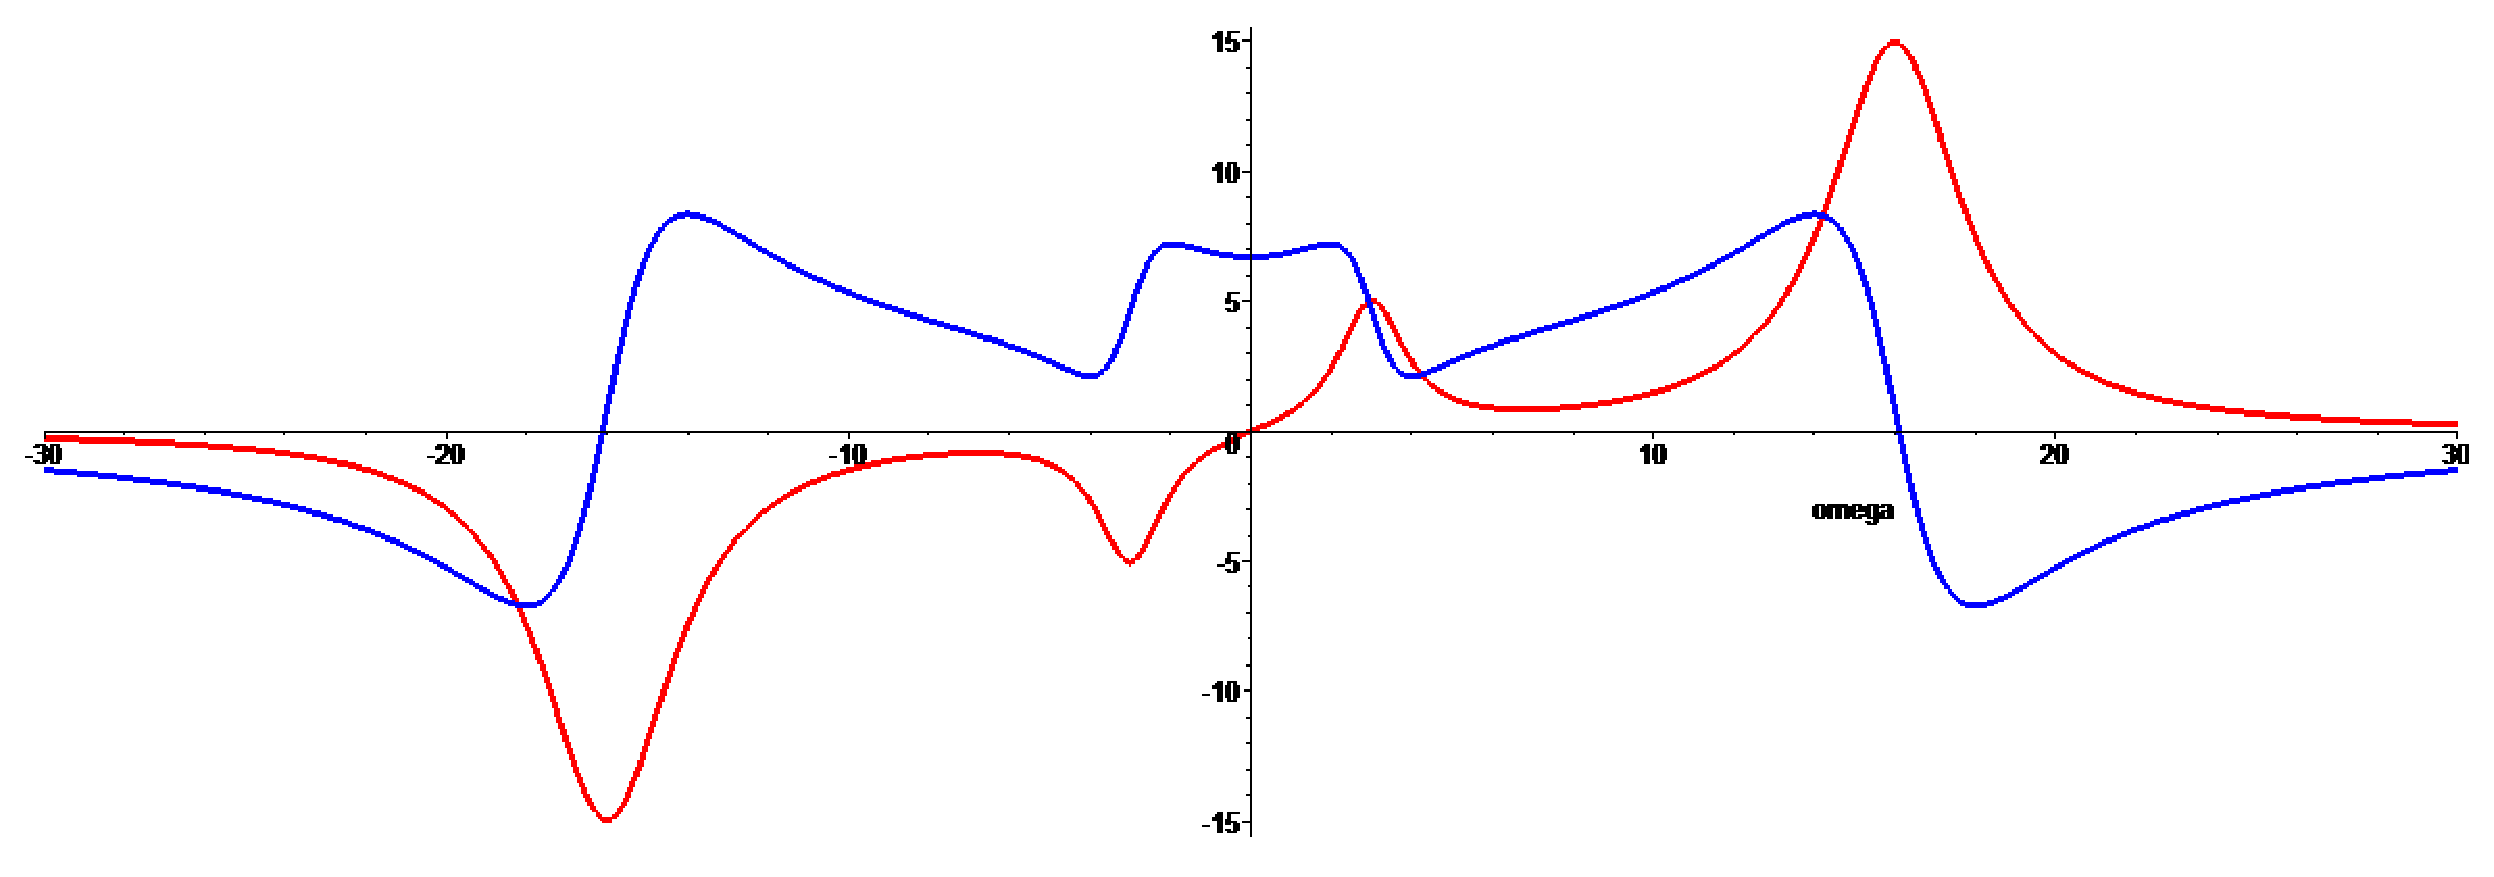
\includegraphics[width=170mm]{img/qp_plot.eps}
{\small 
[Figure 2.5.1a] Quantum-perturbative plot for 3-level model of with
arbitrary (non-physical) parameters. Red plot is for the imaginary and
the blue plot is for the real part on linear susceptibility.}





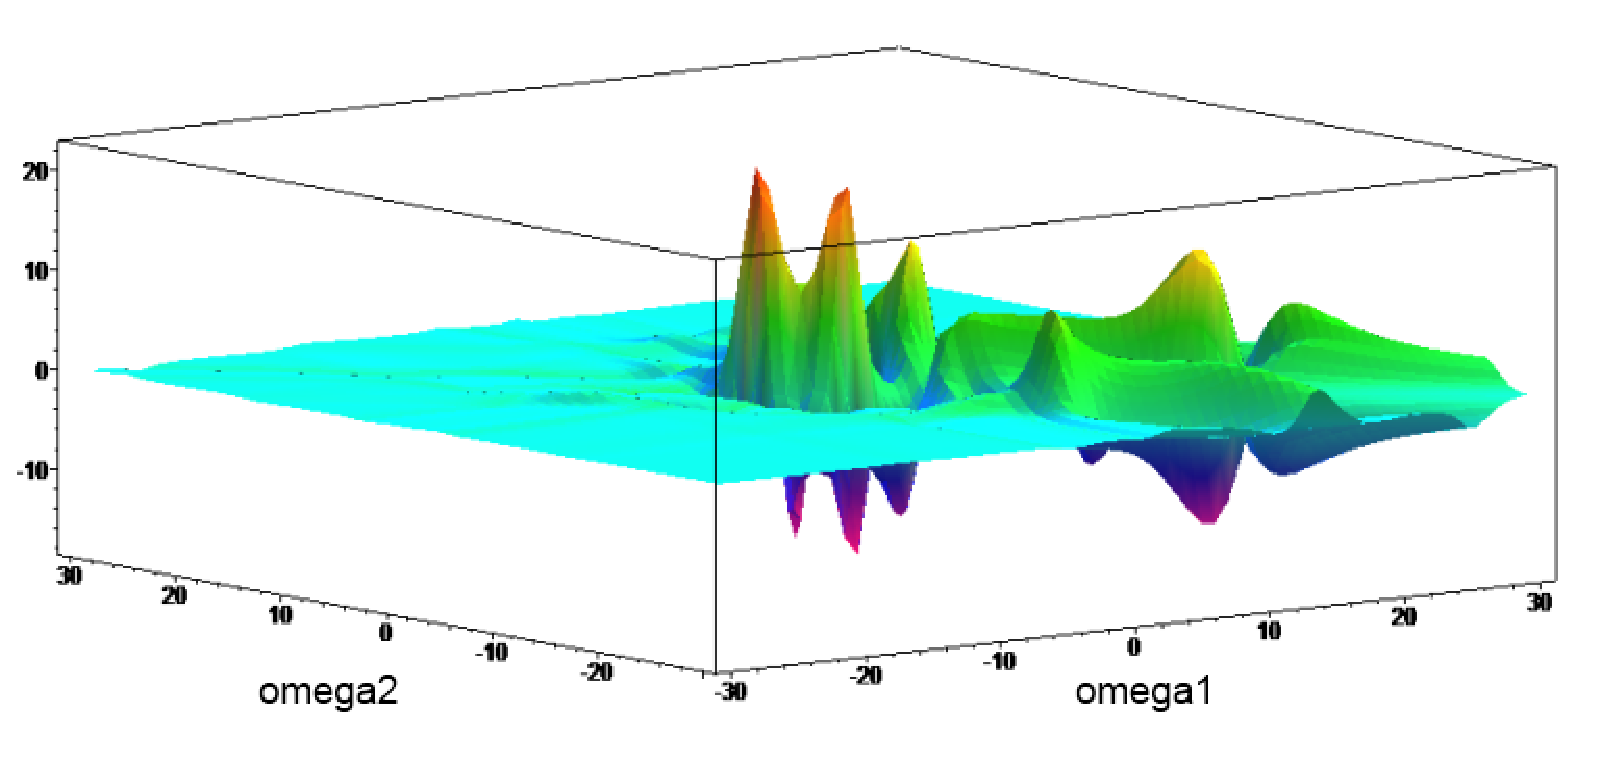
\includegraphics[width=170mm]{img/qp_3da.eps}
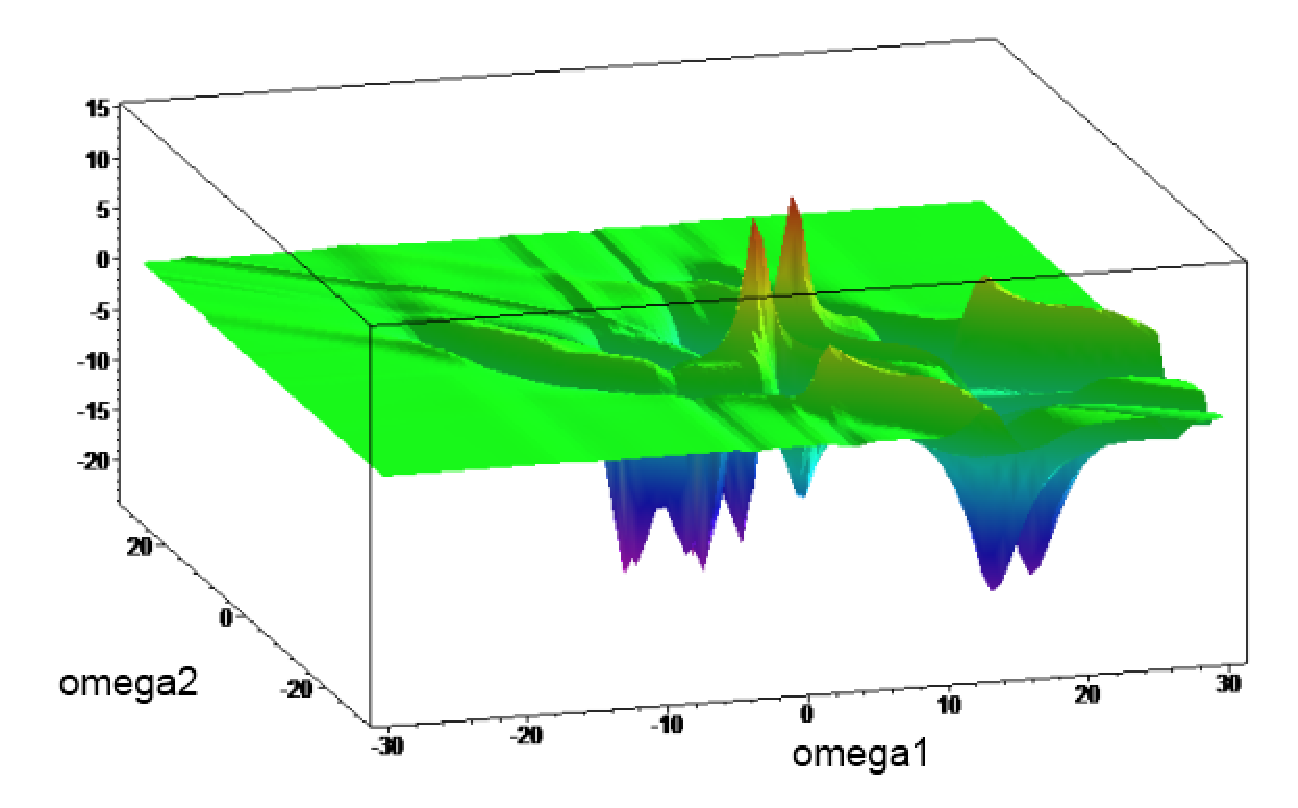
\includegraphics[width=170mm]{img/qp_3db.eps}



{\small [Figure 2.5.1b] Quantum-perturbative plot for 3-level model of
with arbitrary (non-physical) parameters. Red plot is for the
imaginary and the blue plot is for the real part on second-order
susceptibility.}





\textit{Brief overview of the perturbative model}




\subsection{Derivation of the Kramers-Kronig  relations for
simple quantum-perturbative model}



Using the (2.4.4a-b) equations for the just showed model - we will
connect the real and imaginary part of quantum-perturbative derived
optical susceptibilities using the Hilbert transform form:





(2.6.1a) 
\mapleinline{inert}{2d}{Re(chi[1,j,k](omega[p]) =
P/Pi*int(Im(chi[1,j,k](Omega))/(Omega-omega[p]),Omega = -infinity ..
infinity));}{%
$\Re  \left(  \! {\chi _{1, \,j, \,k}}({\omega _{p}})=\frac {P\,
\int _{ - \infty }^{\infty }\frac {\Im ({\chi _{1, \,j, \,k}}(
\Omega ))}{\Omega  - {\omega _{p}}}\,d\Omega }{\pi } \!  \right) 
$%
}
(2.6.1b) 
\mapleinline{inert}{2d}{Im(chi[1,j,k](omega[p]) =
(-P/Pi)*int(Re(chi[1,j,k](Omega))/(Omega-omega[p]),Omega = -infinity
.. infinity));}{%
$\Im  \left(  \! {\chi _{1, \,j, \,k}}({\omega _{p}})=( - \frac {
P}{\pi })\,\int _{ - \infty }^{\infty }\frac {\Re ({\chi _{1, \,j
, \,k}}(\Omega ))}{\Omega  - {\omega _{p}}}\,d\Omega  \! 
 \right) $%
}





(2.6.2a) 
\mapleinline{inert}{2d}{Re(chi[2, i, j, k](omega[p]+omega[q],omega[p],omega[q]) =
P/Pi*int(int(Im(chi[2,i,j,k](Omega[p]+Omega[q],Omega[p],Omega[q]))/((O
mega[p]-omega[p])*(Omega[q]-omega[q])),Omega[p] = -infinity ..
infinity),Omega[q] = -infinity .. infinity));}{%
$\Re  \left(  \! {\chi _{2, \,i, \,j, \,k}}({\omega _{p}} + {
\omega _{q}}, \,{\omega _{p}}, \,{\omega _{q}})=\frac {P\,\int _{
 - \infty }^{\infty }\int _{ - \infty }^{\infty }\frac {\Im ({
\chi _{2, \,i, \,j, \,k}}({\Omega _{p}} + {\Omega _{q}}, \,{
\Omega _{p}}, \,{\Omega _{q}}))}{({\Omega _{p}} - {\omega _{p}})
\,({\Omega _{q}} - {\omega _{q}})}\,d{\Omega _{p}}\,d{\Omega _{q}
}}{\pi } \!  \right) $%
}
(2.6.2b) 
\mapleinline{inert}{2d}{Im(chi[2,i,j,k](omega[p]+omega[q],omega[p],omega[q]) =
P/(-Pi)*int(int(Re(chi[2,i,j,k](Omega[p]+Omega[q],Omega[p],Omega[q]))/
((Omega[p]-omega[p])*(Omega[q]-omega[q])),Omega[p] = -infinity ..
infinity),Omega[q] = -infinity .. infinity));}{%
$\Im  \left(  \! {\chi _{2, \,i, \,j, \,k}}({\omega _{p}} + {
\omega _{q}}, \,{\omega _{p}}, \,{\omega _{q}})=\frac {P\,\int _{
 - \infty }^{\infty }\int _{ - \infty }^{\infty }\frac {\Re ({
\chi _{2, \,i, \,j, \,k}}({\Omega _{p}} + {\Omega _{q}}, \,{
\Omega _{p}}, \,{\Omega _{q}}))}{({\Omega _{p}} - {\omega _{p}})
\,({\Omega _{q}} - {\omega _{q}})}\,d{\Omega _{p}}\,d{\Omega _{q}
}}{ - \pi } \!  \right) $%
}   





(2.6.3a) 
\mapleinline{inert}{2d}{Re(chi[3,i,j,k,l](omega[p]+omega[q]+omega[r],omega[p],omega[q],omega[
r]) =
P/Pi*int(int(int(Im(chi[3,i,j,k,l](Omega[p]+Omega[q]+Omega[r],Omega[p]
,Omega[q],Omega[r]))/((Omega[p]-omega[p])*(Omega[q]-omega[q])*(Omega[r
]-omega[r])),Omega[p] = -infinity .. infinity),Omega[q] = -infinity ..
infinity),Omega[r] = -infinity .. infinity));}{%
$\Re  \left(  \! {\chi _{3, \,i, \,j, \,k, \,l}}({\omega _{p}} + 
{\omega _{q}} + {\omega _{r}}, \,{\omega _{p}}, \,{\omega _{q}}, 
\,{\omega _{r}})=\frac {P\,\int _{ - \infty }^{\infty }\int _{ - 
\infty }^{\infty }\int _{ - \infty }^{\infty }\frac {\Im ({\chi 
_{3, \,i, \,j, \,k, \,l}}({\Omega _{p}} + {\Omega _{q}} + {\Omega
 _{r}}, \,{\Omega _{p}}, \,{\Omega _{q}}, \,{\Omega _{r}}))}{({
\Omega _{p}} - {\omega _{p}})\,({\Omega _{q}} - {\omega _{q}})\,(
{\Omega _{r}} - {\omega _{r}})}\,d{\Omega _{p}}\,d{\Omega _{q}}\,
d{\Omega _{r}}}{\pi } \!  \right) $%
}
(2.6.3a)
\mapleinline{inert}{2d}{Im(chi[3,i,j,k,l](omega[p]+omega[q]+omega[r],omega[p],omega[q],omega[
r]) =
P/(-Pi)*int(int(int(Im(chi[3,i,j,k,l](Omega[p]+Omega[q]+Omega[r],Omega
[p],Omega[q],Omega[r]))/((Omega[p]-omega[p])*(Omega[q]-omega[q])*(Omeg
a[r]-omega[r])),Omega[p] = -infinity .. infinity),Omega[q] = -infinity
.. infinity),Omega[r] = -infinity .. infinity));}{%
$\Im  \left(  \! {\chi _{3, \,i, \,j, \,k, \,l}}({\omega _{p}} + 
{\omega _{q}} + {\omega _{r}}, \,{\omega _{p}}, \,{\omega _{q}}, 
\,{\omega _{r}})=\frac {P\,\int _{ - \infty }^{\infty }\int _{ - 
\infty }^{\infty }\int _{ - \infty }^{\infty }\frac {\Im ({\chi 
_{3, \,i, \,j, \,k, \,l}}({\Omega _{p}} + {\Omega _{q}} + {\Omega
 _{r}}, \,{\Omega _{p}}, \,{\Omega _{q}}, \,{\Omega _{r}}))}{({
\Omega _{p}} - {\omega _{p}})\,({\Omega _{q}} - {\omega _{q}})\,(
{\Omega _{r}} - {\omega _{r}})}\,d{\Omega _{p}}\,d{\Omega _{q}}\,
d{\Omega _{r}}}{ - \pi } \!  \right) $%
}  





In further chapters we will put this equations into some numerical
evaluations.





\textit{Mathematical derivation of the Kramers-Kronig relations for
simple perturbative model.}




\subsection{Overview of the other models}



D. C. Hutchings et al. [23] have proposed the models for particular
nonlinear absorption processes as following:
Here we would like to state  - only from the physical point of view -
without formulating advanced mathematical models - that the theory of
K-K relations - or to say it precisely - the conjugated pairs of
Hilbert transforms - need to be structured and defined generaly for
both the linear and nonlinear case - there must be on valid theory -
it is not a good situation - when we start from one theory and then
''modify'' it for some extra case - because it leads to misunderstanding
in general. As the title of this thesis contains the word -
understanding - we should at least try to express a new, general
theory of optical phenomena - because it is ''only and even'' - the
interaction of a chemical molecules with incoming photons in short or
long period of time.





(2.7.1) Two-photon absorption: 
\mapleinline{inert}{2d}{F[TPA](x[1],x[2]) =
(x[1]+x[2]-1)^(3/2)/(2^7)/x[1]/(x[2]^2)*(1/x[1]+1/x[2])^2;}{%
${F_{\mathit{TPA}}}({x_{1}}, \,{x_{2}})=\frac {({x_{1}} + {x_{2}}
 - 1)^{(\frac {3}{2})}\,(\frac {1}{{x_{1}}} + \frac {1}{{x_{2}}})
^{2}}{2^{7}\,{x_{1}}\,{x_{2}}^{2}}$%
}
(2.7.2) Raman: 
\mapleinline{inert}{2d}{F[Raman](x[1],x[2]) =
(x[1]-x[2]-1)^(3/2)/(2^7)/x[1]/(x[2]^2)*(1/x[1]-1/x[2])^2;}{%
${F_{\mathit{Raman}}}({x_{1}}, \,{x_{2}})=\frac {({x_{1}} - {x_{2
}} - 1)^{(\frac {3}{2})}\,(\frac {1}{{x_{1}}} - \frac {1}{{x_{2}}
})^{2}}{2^{7}\,{x_{1}}\,{x_{2}}^{2}}$%
}
(2.7.3) Linear stark: 
\mapleinline{inert}{2d}{F[LS](x[1],x[2]) = -(x[1]-1)^(3/2)/(2^6)/x[1]/(x[2]^2);}{%
${F_{\mathit{LS}}}({x_{1}}, \,{x_{2}})= - \frac {({x_{1}} - 1)^{(
\frac {3}{2})}}{2^{6}\,{x_{1}}\,{x_{2}}^{2}}$%
}(
\mapleinline{inert}{2d}{1/(x[2]^2);}{%
$\frac {1}{{x_{2}}^{2}}$%
})
(2.7.4) Quadratic stark: 
\mapleinline{inert}{2d}{F[QS](x[1],x[2]) =
-1/(2^10)/x[1]/(x[2]^2)/((x[1]-1)^(1/2))*(1/(x[1]-x[2])+1/(x[1]+x[2]))
;}{%
${F_{\mathit{QS}}}({x_{1}}, \,{x_{2}})= - \frac {1\,(\frac {1}{{x
_{1}} - {x_{2}}} + \frac {1}{{x_{1}} + {x_{2}}})}{2^{10}\,{x_{1}}
\,{x_{2}}^{2}\,({x_{1}} - 1)^{(\frac {1}{2})}}$%
}  





Where in all (2.7.1-4) equations we assume that:





(2.7.5) 
\mapleinline{inert}{2d}{x[1] = h*omega[1]/E[g];}{%
${x_{1}}=\frac {h\,{\omega _{1}}}{{E_{g}}}$%
}, 
\mapleinline{inert}{2d}{x[2] = h*omega[2]/E[g];}{%
${x_{2}}=\frac {h\,{\omega _{2}}}{{E_{g}}}$%
}





where:
\mapleinline{inert}{2d}{E[g];}{%
${E_{g}}$%
} - the edge absorption energy, a nonconstant parameter





\textit{Introduction into variety of other models avaiable in physics
of the nonlinear optics.}




\begin{mapleinput}
\mapleinline{active}{1d}{Should I write more on particular models?}{%
}
\end{mapleinput}



\subsection{Derivation of the Kramers-Kronig relations for
other models}



D. C. Hutchings et al. [23] have also proposed the analytical
equations based on (2.7.1-4) aquired with Hilbert transform 





(2.8.1) 
\mapleinline{inert}{2d}{G(x) = P/Pi*int(F(y,x)/(y-x),y = -infinity .. infinity);}{%
$\mathrm{G}(x)=\frac {P\,\int _{ - \infty }^{\infty }\frac {
\mathrm{F}(y, \,x)}{y - x}\,dy}{\pi }$%
} 





And they obtained the following results:





(2.8.2) Two-photon absorption: 
\mapleinline{inert}{2d}{G[TPA](x);}{%
${G_{\mathit{TPA}}}(x)$%
} = [1/
\mapleinline{inert}{2d}{(2*x)^6;}{%
$(2\,x)^{6}$%
})[-
\mapleinline{inert}{2d}{3/8;}{%
$\frac {3}{8}$%
}
\mapleinline{inert}{2d}{x^2;}{%
$x^{2}$%
}
\mapleinline{inert}{2d}{(1-x)^(-1/2);}{%
$(1 - x)^{( - \frac {1}{2})}$%
} + 3x
\mapleinline{inert}{2d}{(1-x)^(1/2);}{%
$(1 - x)^{(\frac {1}{2})}$%
}-2
\mapleinline{inert}{2d}{(1-x)^(3/2);}{%
$(1 - x)^{(\frac {3}{2})}$%
}+2
\mapleinline{inert}{2d}{Theta(1-2*x);}{%
$\Theta (1 - 2\,x)$%
}
\mapleinline{inert}{2d}{(1-2*x)^(3/2);}{%
$(1 - 2\,x)^{(\frac {3}{2})}$%
}] ( where 
\mapleinline{inert}{2d}{Theta(t);}{%
$\Theta (t)$%
} - Heaviside function )
(2.8.3) Raman: 
\mapleinline{inert}{2d}{G[RAMAN](x);}{%
${G_{\mathit{RAMAN}}}(x)$%
} = [1/
\mapleinline{inert}{2d}{(2*x)^6;}{%
$(2\,x)^{6}$%
}][-
\mapleinline{inert}{2d}{3/8;}{%
$\frac {3}{8}$%
}
\mapleinline{inert}{2d}{x^2;}{%
$x^{2}$%
}
\mapleinline{inert}{2d}{(1+x)^(-1/2);}{%
$(1 + x)^{( - \frac {1}{2})}$%
} - 3x
\mapleinline{inert}{2d}{(1+x)^(1/2);}{%
$(1 + x)^{(\frac {1}{2})}$%
}-2
\mapleinline{inert}{2d}{(1+x)^(3/2);}{%
$(1 + x)^{(\frac {3}{2})}$%
}+2
\mapleinline{inert}{2d}{(1+2*x)^(3/2);}{%
$(1 + 2\,x)^{(\frac {3}{2})}$%
}]
(2.8.4) Linear Stark: 
\mapleinline{inert}{2d}{G[LS](x);}{%
${G_{\mathit{LS}}}(x)$%
} = [1/
\mapleinline{inert}{2d}{(2*x)^6;}{%
$(2\,x)^{6}$%
}][2 - 
\mapleinline{inert}{2d}{(1-x)^(3/2);}{%
$(1 - x)^{(\frac {3}{2})}$%
} - 
\mapleinline{inert}{2d}{(1+x)^(3/2);}{%
$(1 + x)^{(\frac {3}{2})}$%
}]
(2.8.5) Quadratic Stark: 
\mapleinline{inert}{2d}{G[QS](x);}{%
${G_{\mathit{QS}}}(x)$%
} = [1/(
\mapleinline{inert}{2d}{2^10;}{%
$2^{10}$%
}
\mapleinline{inert}{2d}{x^5;}{%
$x^{5}$%
})][
\mapleinline{inert}{2d}{(1-x)^(-1/2)-(1+x)^(-1/2)-1/2*x*(1-x)^(3/2)-1/2*x*(1+x)^(-3/2);}{%
$(1 - x)^{( - \frac {1}{2})} - (1 + x)^{( - \frac {1}{2})} - 
\frac {1\,x\,(1 - x)^{(\frac {3}{2})}}{2} - \frac {1\,x\,(1 + x)
^{( - \frac {3}{2})}}{2}$%
}]





In further chapters we will put this equations into a try. There can
be other models found in literature - but our approach will remaind
the same - check if the model assumed is valid.





\textit{The derived models using the Hilbert transform are presented}




\section{Z-scan Measurments (understanding)}

\subsection{Overview of the z-scan technique}



One of the most important questions being the major motivation of this
thesis is how the theory of Hilbert transform or the Kramers-Kronig
relations can be applied to the data measured with the standard ''open
aperture'' and ''closed aperture'' z-scan technique. In this chapter we
will describe the process of data collection and its translation into
the nonlinear absorption coefficient spectra and nonlinear refraction
index spectra. As mentioned before, since summer 2010 we have set up
the femtosecond z-scan system using a Quantronix Integra regenerative
amplifier operating at 1 kHz and providing appr. 1 mJ, 100 fs, 800 nm
pulses. It is used as a pump to the Palitra optical parametric
amplifier, which, using several different frequency mixing schemes,
can provide the coverage of the 450 - 2000 nm wavelength range. The
best way to describe this set up will be to use Figure 3.1.1a and
Figure 3.1.1b.






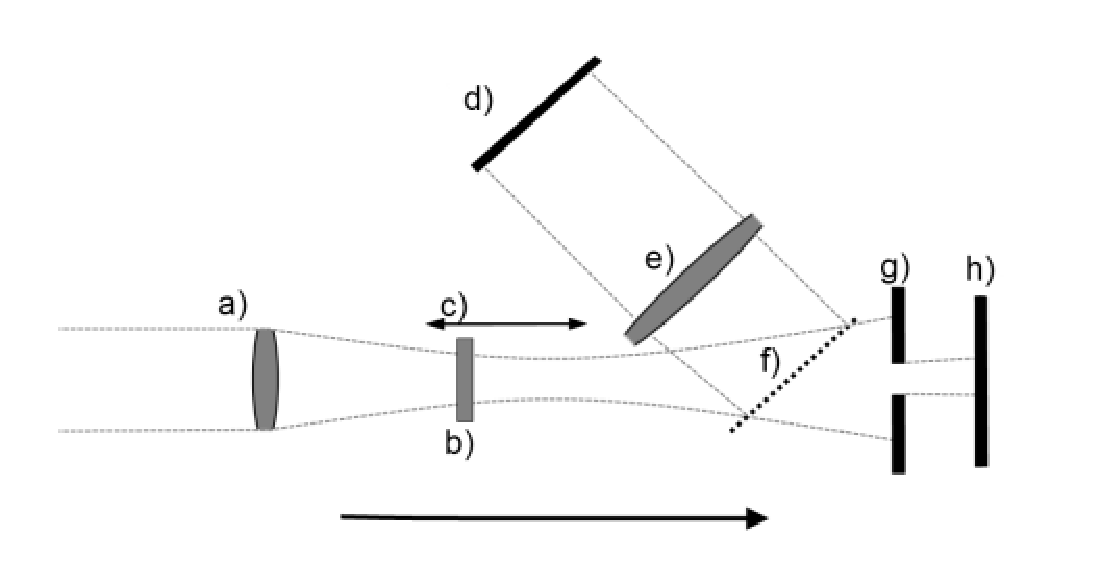
\includegraphics{img/zscan_sch.eps}
[Figure 3.1.1a] The schematic diagram of the main measurement part of
the z-scan experiment
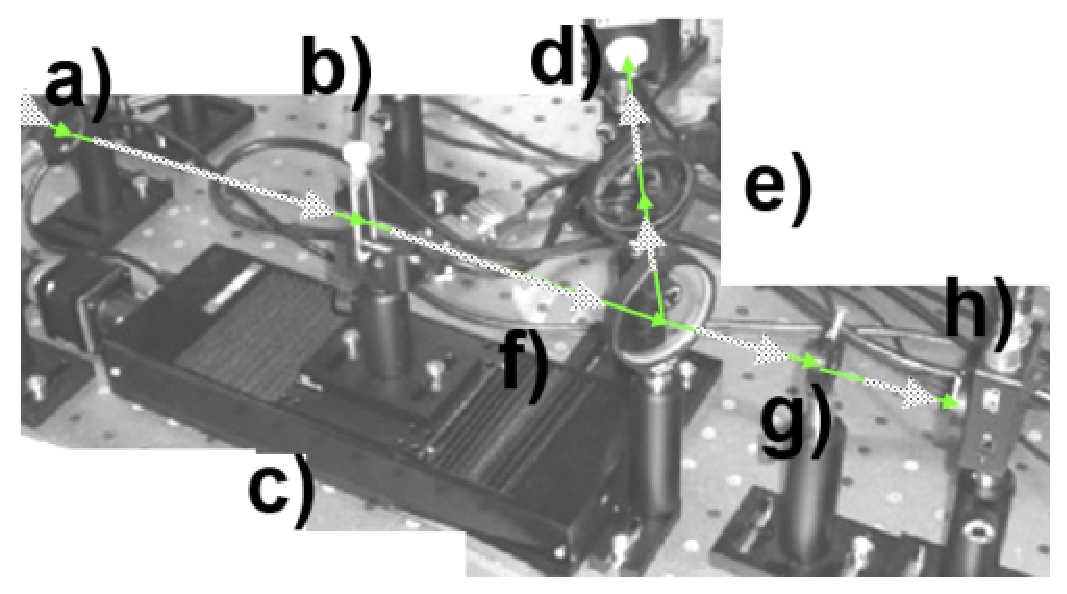
\includegraphics{img/zscan_diag.eps}
[Figure 3.1.1b] The photographic diagram of the main measurement part
of the z-scan experiment.
[Legend for 3.1.1a-b] 
Overview of the main measurement part of the z-scan set-up built at
the Wroclaw University of Technology and being under usage since
summer 2010.
a) FOCUSING LENSE - A laser beam goes through focusing a lense.  \\
b) SAMPLE IN A QUEVETTE - Investigate sample is put into a silica \\
quvette. \\
c) DYNAMIC (MOBILE) STAGE - During experiment the sample changes its
relative position from the lense  \\
d) DETECTOR 1 - Finally the beam reaches the ``Open-aperture'' detector  \\
e) DEFOCUSING LENSE  - ``Open-aperture'' defocuing lense before detector \\
f) BEAM SPLITTER - Laser beam is splitted to pass both through
''open-aperture'' and ''closed aperture'' with a beam splitter \\
g) APERTURE - This is the aperture before the ``Closed-aperture''
detector \\
h) DETECTOR 2 - Finally the beam reaches the ``Closed-aperture''
detector \\





The inventor of the z-scan technique was the Dr. Mansoor Sheik-Bahae
in 1989 [24] and since then many variants of this technique have been
deployed �EZ-Scan�, �White Light z-scan�, �Excite-Probe z-scan"[23].
In a short description - the z-scan technique uses a single laser
beam, a mobile stage and two detectors - for the open and closed
aperture. Using physical model - we can relate the open-aperture
results with the nonlinear absorption and the closed-aperture with the
nonlinear refraction index. The mobile stage moves the sample through
the position focal point of the focusing lense. We therefore obtain
two diagrams - shown on the Figures 3.1.2a-b.





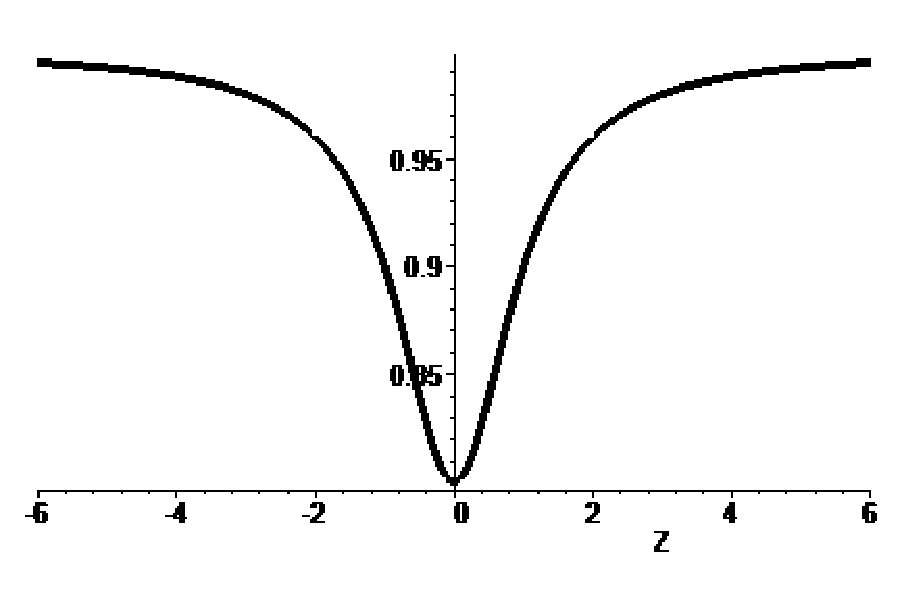
\includegraphics{img/oa_plot.eps}

{\small [Figure 3.1.2a] A typical open-aperture transmittance 
\mapleinline{inert}{2d}{Delta*T(Z);}{%
$\Delta \,\mathrm{T}(Z)$%
} plot in a z-scan experiment, 
where: 
Z - the position of the stage/sample, where 0 position - the focal
point of focusing lense}





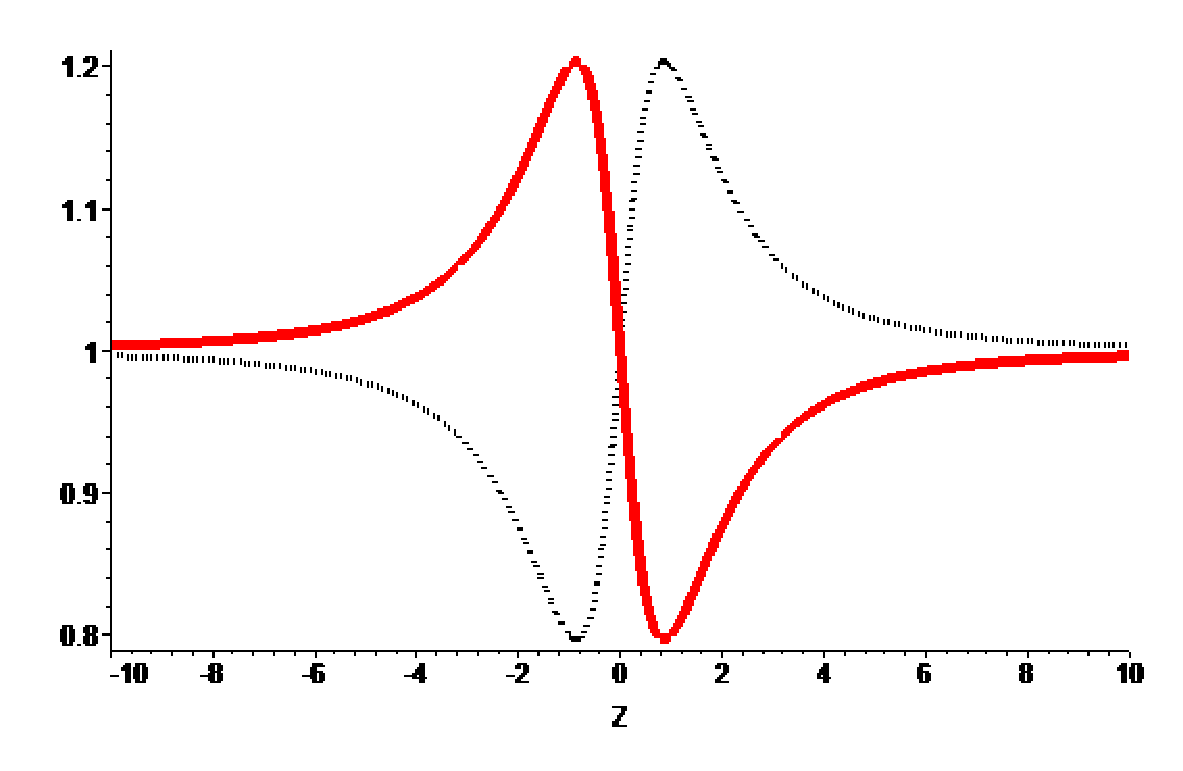
\includegraphics{img/ca_plot.eps}
{\small 
[Figure 3.1.2b] A typical closed-aperture transmittance 
\mapleinline{inert}{2d}{Delta*T(Z);}{%
$\Delta \,\mathrm{T}(Z)$%
} plots in a z-scan experiment, 
where: 
Z - the position of the stage/sample, where 0 position - the focal
point of focusing lense
red (dashed) plot is for material with a positive (negative)
refractive index}





We must hereby stress that what we obtain with one z-scan measurement
is only half a way to calculate one point in the nonlinear spectrum
plot - because a typical sample is held inside a silica cuvette and is
soluted in some solution (for example chloroform or toluen). So
firstly we must measure the solution and an empty silica cuvette
z-scan transmittance plots for each monochromatic wavelength and after
so - perform the z-scan experiment on the investigated sample. 





\textit{Description of the z-scan technique, description of the z-scan
experiment built in Wroclaw, since summer 2010.}




\subsection{Overview of the derivation }

\subsubsection*{Calculation of the nonlinear absorption coefficient:}



As shown of the Figure 3.1.2a the open-aperture trasmittance can be
described with the approximation equation:





(3.2.1) 
\mapleinline{inert}{2d}{Delta*T(Z) =
beta*I[0]*(1-exp(-alpha)*L)/alpha/(2*sqrt(2))/(1+Z^2/((n*Pi*w[0]*2/lam
bda)^2));}{%
$\Delta \,\mathrm{T}(Z)=\frac {\beta \,{I_{0}}\,(1 - e^{( - 
\alpha )}\,L)}{\alpha \,2\,\sqrt{2}\, \left(  \! 1 + \frac {Z^{2}
}{(\frac {n\,\pi \,{w_{0}}\,2}{\lambda })^{2}} \!  \right) }$%
} 
where:
\mapleinline{inert}{2d}{Delta*T(Z);}{%
$\Delta \,\mathrm{T}(Z)$%
} - normalized transmittance of the sample at Z
\mapleinline{inert}{2d}{beta;}{%
$\beta $%
} - two-photon absorption coefficient
\mapleinline{inert}{2d}{I[0];}{%
${I_{0}}$%
} - peak on-axis irradiance at focus
L - sample length
\mapleinline{inert}{2d}{alpha;}{%
$\alpha $%
} - absorption coefficient
n - index of refraction
\mapleinline{inert}{2d}{w[0];}{%
${w_{0}}$%
} - spot size at focus (radius at 
\mapleinline{inert}{2d}{1/exp(2);}{%
$\frac {1}{e^{2}}$%
})
\mapleinline{inert}{2d}{lambda;}{%
$\lambda $%
} - laser wavelength
Z - position of sample with respect to the focal position





We obtain the two-photon absorption coefficient while standard (f.e.
least squares) fitting the measured open-aperture 
\mapleinline{inert}{2d}{beta;}{%
$\beta $%
} plot. This is of cource also not the complete truth, because with
some advanced models we can also obtain other absorptive
nonlinearities. In a short description - the multiphoton absorption
can be assumed when the closed-apperture peak is supressed, but
unfortunatelly the absorption saturation has got just the opposite
effect. So the z-scan technique gives only the simple information
about the nonlinear absorption processes.




\subsubsection*{Calculation of the nonlinear refraction index:}



On the Figure 3.1.2b we can see the closed-aperture trasmittance plot
with respect to the sample position Z. It has a characteristic shape
of peak trailing the valled or the valley trailing the peak if the 
\mapleinline{inert}{2d}{n[2];}{%
${n_{2}}$%
} sign is negative. What now interest us is the difference between the
peak and valley amplitude - we will call it 
\mapleinline{inert}{2d}{Delta*T[pv];}{%
$\Delta \,{T_{\mathit{pv}}}$%
}. From this difference we can calculate the on-axis peak nonlinear
phase shift with sample at focus 
\mapleinline{inert}{2d}{Delta*Phi[0];}{%
$\Delta \,{\Phi _{0}}$%
}





(3.2.2) 
\mapleinline{inert}{2d}{abs(Delta*Phi[0]) = Delta*T[pv]/(.407*(1-S)^.27);}{%
$ \left|  \! \,\Delta \,{\Phi _{0}}\, \!  \right| =\frac {\Delta 
\,{T_{\mathit{pv}}}}{\mbox{.407}\,(1 - S)^{\mbox{.27}}}$%
}
where:
S - fraction of beam transmitted by the aperture
\mapleinline{inert}{2d}{Delta*T[pv];}{%
$\Delta \,{T_{\mathit{pv}}}$%
} - change in normalized transmittance between peak and valley.





Now we can estimate the refraction index from equation:





(3.2.3) 
\mapleinline{inert}{2d}{n[2] = lambda/2/Pi*Delta*Phi[0]/I[0]/((1-exp(-alpha)*L)/alpha);}{%
${n_{2}}=\frac {\lambda \,\Delta \,{\Phi _{0}}}{2\,\pi \,{I_{0}}
\,\frac {1 - e^{( - \alpha )}\,L}{\alpha }}$%
}





where:
\mapleinline{inert}{2d}{Delta*Phi[0];}{%
$\Delta \,{\Phi _{0}}$%
} - on-axis peak nonlinear phase shift with sample at focus
\mapleinline{inert}{2d}{I[0];}{%
${I_{0}}$%
} - peak on-axis irradiance at focus
L - sample length
\mapleinline{inert}{2d}{alpha;}{%
$\alpha $%
} - absorption coefficient
\mapleinline{inert}{2d}{lambda;}{%
$\lambda $%
} - laser wavelength





With data points collected for each wavelength we may obtain the full
spectral plot for both nonlinear absorption coefficient and nonlinear
refraction index - due to the z-scan measurements.





\textit{Description how the gathered data is transformed into final
chart. Some mathematical derivations.}




\subsection{Definition of the main problems}



A typical z-scan experiment consists of the measurement routines with
number more or less around 15-20 different wavelength. One z-scan
measurement usually takes between 5 to 10 minutes and together with:
a) long laser calibration process after each change of wavelength 
b) silica and empty-solution measurement
c) measurement of a typical set of 10-20 measured cuvette samples 
it may take many days or even weeks to complete one measurement - so
even such a simple routine is rather time-demanding. Therefore we are
interested in optimizing the method, the physical theory understanding
and the numerical precision, because the general error cumulates with
the laser nonstability, method approximation error, fitting and
numerical calculations error. 



A typical plot containing the z-scan measurement for  the close
aperture, open aperture and the laser reference is shown in the Figure
3.3.1:





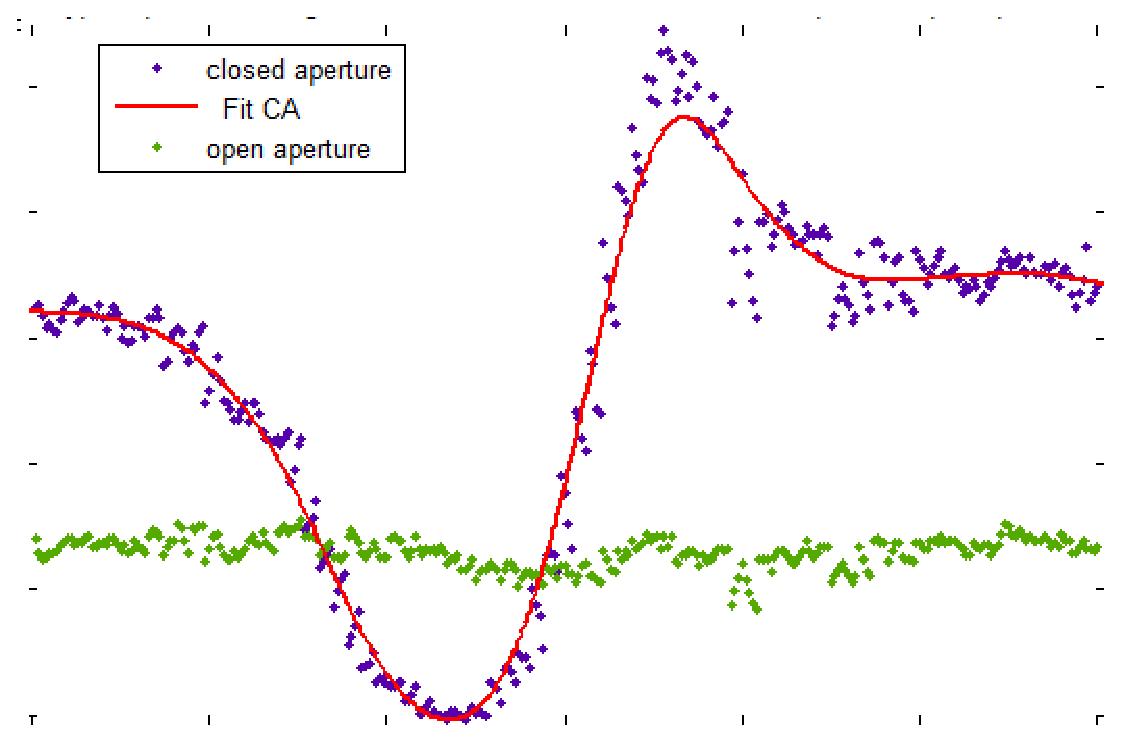
\includegraphics{img/zscan_both.eps}
{\small [Figure 3.3.1] A typical plot for both close and open aperture
with respect to the sample position Z and with the fit splineline.}





\textit{Discussion about the z-scan technique, its advantages and
disadvantages for determination both real and imaginary part of
nonlinear susceptibility.}




\begin{mapleinput}
\mapleinline{active}{1d}{1. Is it not to short? Need to ask Prof. Samoc. Maybe we should also
describe the ''White-Light or time-resolved ZScan''?  }{%
}
\end{mapleinput}



\begin{mapleinput}
\mapleinline{active}{1d}{2. Is there any model for z-scan experiment?}{%
}
\end{mapleinput}



\section{Simpson and trapezoidal quadrature combined with cubic
interpolation - HTRAN (solving)}

\subsection{Overview of the HTRAN}



We define the tabular-based function HTRAN and show its theoretical
fundaments here. It has been implemented in MATLAB environment, and
its source code is avaiable in Appendix A.1
We shall start from the simplest possible numerical calculation of
integral - so the simpson and trapezoidal quadrature. The algorithm is
based on report by I. J. Weinberg [18] written for CDC 6600
supercomputer, but the difference is that it does not require the
input function to be even. We first start from the modification of the
main Hilbert transform equation:





(4.1.1) 
\mapleinline{inert}{2d}{HT(omega) = P/Pi*int(R(Omega)/(Omega-omega),Omega = -infinity ..
infinity);}{%
$\mathrm{HT}(\omega )=\frac {P\,\int _{ - \infty }^{\infty }
\frac {\mathrm{R}(\Omega )}{\Omega  - \omega }\,d\Omega }{\pi }$%
} = 
\mapleinline{inert}{2d}{lim[proc (epsilon) options operator, arrow; 0 end
proc](int(R(Omega)/(Omega-omega),Omega = -infinity ..
omega-epsilon)+int(R(Omega)/(Omega-omega),Omega = omega+epsilon ..
infinity));}{%
${\mathit{lim}_{\varepsilon \rightarrow 0}} \left(  \! \int _{ - 
\infty }^{\omega  - \varepsilon }\frac {\mathrm{R}(\Omega )}{
\Omega  - \omega }\,d\Omega  + \int _{\omega  + \varepsilon }^{
\infty }\frac {\mathrm{R}(\Omega )}{\Omega  - \omega }\,d\Omega 
 \!  \right) $%
} as the integral uses the Cauchy Principal Value

We firstly observe, that:

(4.1.2) '' 
\mapleinline{inert}{2d}{omega;}{%
$\omega $%
} : 
\mapleinline{inert}{2d}{P*int(1/(Omega-omega),Omega = -infinity .. infinity) = 0;}{%
$P\,\int _{ - \infty }^{\infty }\frac {1}{\Omega  - \omega }\,d
\Omega =0$%
}

Making any number of multiplications of (4.1.2) does not change the
fact it will equal zero - so we may obtain a new form of the (4.1.1)
integral:

(4.1.3) 
\mapleinline{inert}{2d}{HT(omega) = P/Pi*int((R(Omega)-R(omega))/(Omega-omega),Omega =
-infinity .. infinity);}{%
$\mathrm{HT}(\omega )=\frac {P\,\int _{ - \infty }^{\infty }
\frac {\mathrm{R}(\Omega ) - \mathrm{R}(\omega )}{\Omega  - 
\omega }\,d\Omega }{\pi }$%
}


As the proposed HTRAN method will take two arguments: 
F[] - the tables of abscissas and R[] - the tabular ordinates 
- we will assume that the function vanishes anywhere else - namely it
equals zero:

(4.1.4) '' (
\mapleinline{inert}{2d}{omega;}{%
$\omega $%
} \TEXTsymbol{<} 
\mapleinline{inert}{2d}{F[1];}{%
${F_{1}}$%
} and 
\mapleinline{inert}{2d}{omega;}{%
$\omega $%
} \TEXTsymbol{>} 
\mapleinline{inert}{2d}{F[N];}{%
${F_{N}}$%
}) : 
\mapleinline{inert}{2d}{R(omega) = 0;}{%
$\mathrm{R}(\omega )=0$%
}
From (4.1.3) and (4.1.4) we obtain:
(4.1.5) 
\mapleinline{inert}{2d}{HT(omega) = (int(-R(omega)/(Omega-omega),Omega = -infinity ..
F[1])+int((R(Omega)-R(omega))/(Omega-omega),Omega = F[1] ..
F[N])+int(-R(omega)/(Omega-omega),Omega = F[N] .. infinity))/Pi;}{%
$\mathrm{HT}(\omega )=\frac {\int _{ - \infty }^{{F_{1}}} - 
\frac {\mathrm{R}(\omega )}{\Omega  - \omega }\,d\Omega  + \int 
_{{F_{1}}}^{{F_{N}}}\frac {\mathrm{R}(\Omega ) - \mathrm{R}(
\omega )}{\Omega  - \omega }\,d\Omega  + \int _{{F_{N}}}^{\infty 
} - \frac {\mathrm{R}(\omega )}{\Omega  - \omega }\,d\Omega }{\pi
 }$%
}

We shall also remember, that:

(4.1.6) '' 
\mapleinline{inert}{2d}{M;}{%
$M$%
} :
\mapleinline{inert}{2d}{int(1/(Omega-omega),Omega = -infinity ..
omega-M)+int(1/(Omega-omega),Omega = omega+M .. infinity) = 0;}{%
$\int _{ - \infty }^{\omega  - M}\frac {1}{\Omega  - \omega }\,d
\Omega  + \int _{\omega  + M}^{\infty }\frac {1}{\Omega  - \omega
 }\,d\Omega =0$%
}





As 
\mapleinline{inert}{2d}{`in`(omega,[F[1], F[N]]);}{%
$\omega \,\ \textbf{in}\ \,[{F_{1}}, \,{F_{N}}]$%
} we will now consider two conditions - that takes into account the
position of 
\mapleinline{inert}{2d}{omega;}{%
$\omega $%
} in relation to 
\mapleinline{inert}{2d}{F[1];}{%
${F_{1}}$%
} and 
\mapleinline{inert}{2d}{F[N];}{%
${F_{N}}$%
}. We have two posibilities:





(4.1.7a) 
\mapleinline{inert}{2d}{omega-F[1] < F[N]-omega;}{%
$\omega  - {F_{1}} < {F_{N}} - \omega $%
}, which means that 
\mapleinline{inert}{2d}{omega;}{%
$\omega $%
} is placed closer to 
\mapleinline{inert}{2d}{F[1];}{%
${F_{1}}$%
} on the real axis
(4.1.7b) 
\mapleinline{inert}{2d}{F[N]-omega <= omega-F[1];}{%
${F_{N}} - \omega \leq \omega  - {F_{1}}$%
}, which is the opposite case and it is closer to 
\mapleinline{inert}{2d}{F[N];}{%
${F_{N}}$%
}.





Each of these two cases leads to results obtained in (4.1.8a-b) we
have:





(4.1.8a) 
\mapleinline{inert}{2d}{HT(omega) = ((int(-R(omega)/(Omega-omega),Omega = 2*omega-F[N] ..
F[1])+int((R(Omega)-R(omega))/(Omega-omega),Omega = F[1] .. F[N]))/Pi
=
(-R(omega)*ln((F[1]-omega)/(omega-F[N]))+int((R(Omega)-R(omega))/(Omeg
a-omega),Omega = F[1] .. F[N]))/Pi);}{%
$\mathrm{HT}(\omega )= \left(  \! \frac {\int _{2\,\omega  - {F_{
N}}}^{{F_{1}}} - \frac {\mathrm{R}(\omega )}{\Omega  - \omega }\,
d\Omega  + \int _{{F_{1}}}^{{F_{N}}}\frac {\mathrm{R}(\Omega ) - 
\mathrm{R}(\omega )}{\Omega  - \omega }\,d\Omega }{\pi }=\frac {
 - \mathrm{R}(\omega )\,\mathrm{ln}(\frac {{F_{1}} - \omega }{
\omega  - {F_{N}}}) + \int _{{F_{1}}}^{{F_{N}}}\frac {\mathrm{R}(
\Omega ) - \mathrm{R}(\omega )}{\Omega  - \omega }\,d\Omega }{\pi
 } \!  \right) $%
}
(4.1.8b) 
\mapleinline{inert}{2d}{HT(omega) = ((int((R(Omega)-R(omega))/(Omega-omega),Omega = F[1] ..
F[N])+int((-R(omega))/(Omega-omega),Omega = F[N] .. 2*omega-F[1]))/Pi
= (int((R(Omega)-R(omega))/(Omega-omega),Omega = F[1] ..
F[N])-R(omega)*ln((omega-F[1])/(F[N]-omega)))/Pi);}{%
$\mathrm{HT}(\omega )= \left(  \! \frac {\int _{{F_{1}}}^{{F_{N}}
}\frac {\mathrm{R}(\Omega ) - \mathrm{R}(\omega )}{\Omega  - 
\omega }\,d\Omega  + \int _{{F_{N}}}^{2\,\omega  - {F_{1}}}
\frac { - \mathrm{R}(\omega )}{\Omega  - \omega }\,d\Omega }{\pi 
}=\frac {\int _{{F_{1}}}^{{F_{N}}}\frac {\mathrm{R}(\Omega ) - 
\mathrm{R}(\omega )}{\Omega  - \omega }\,d\Omega  - \mathrm{R}(
\omega )\,\mathrm{ln}(\frac {\omega  - {F_{1}}}{{F_{N}} - \omega 
})}{\pi } \!  \right) $%
}





And we can see that both the (4.1.8a-b) derivations lead to the same
result:





(4.1.9) 
\mapleinline{inert}{2d}{HT(omega) =
(-R(omega)*ln((omega-F[1])/(F[N]-omega))+int((R(Omega)-R(omega))/(Omeg
a-omega),Omega = F[1] .. F[N]))/Pi;}{%
$\mathrm{HT}(\omega )=\frac { - \mathrm{R}(\omega )\,\mathrm{ln}(
\frac {\omega  - {F_{1}}}{{F_{N}} - \omega }) + \int _{{F_{1}}}^{
{F_{N}}}\frac {\mathrm{R}(\Omega ) - \mathrm{R}(\omega )}{\Omega 
 - \omega }\,d\Omega }{\pi }$%
}





We also observe, that:





(4.1.10) 
\mapleinline{inert}{2d}{`in`(omega,[F[1], F[N]]);}{%
$\omega \,\ \textbf{in}\ \,[{F_{1}}, \,{F_{N}}]$%
} =\TEXTsymbol{>}
\mapleinline{inert}{2d}{And(0 < omega-F[1],0 < F[N]-omega);}{%
$\mathrm{And}(0 < \omega  - {F_{1}}, \,0 < {F_{N}} - \omega )$%
} =\TEXTsymbol{>} 
\mapleinline{inert}{2d}{0 < (omega-F[1])/(F[N]-omega);}{%
$0 < \frac {\omega  - {F_{1}}}{{F_{N}} - \omega }$%
}  =\TEXTsymbol{>} 
\mapleinline{inert}{2d}{ln((omega-F[1])/(F[N]-omega));}{%
$\mathrm{ln}(\frac {\omega  - {F_{1}}}{{F_{N}} - \omega })$%
}  will have real value. 





What now interest us the most is the integral:





(4.1.11) 
\mapleinline{inert}{2d}{Y(omega) = int((R(Omega)-R(omega))/(Omega-omega),Omega = F[1] ..
F[N]);}{%
$\mathrm{Y}(\omega )=\int _{{F_{1}}}^{{F_{N}}}\frac {\mathrm{R}(
\Omega ) - \mathrm{R}(\omega )}{\Omega  - \omega }\,d\Omega $%
}





As the integrand in (4.1.11) never explodes - we will calculate it
numerically. We will need to prepare ourselves to omit some
difficulties - as when denominators equals zero. In algorithm we are
preparing a new set of 
\mapleinline{inert}{2d}{F[x];}{%
${F_{x}}$%
} values, which are just a simple midways of 
\mapleinline{inert}{2d}{omega;}{%
$\omega $%
} defined:





(4.1.12) 
\mapleinline{inert}{2d}{F[x,k] = (F[k]+F[k+1])/2;}{%
${F_{x, \,k}}=\frac {{F_{k}} + {F_{k + 1}}}{2}$%
} for k = 
\mapleinline{inert}{2d}{1 .. N-1;}{%
$1 .. N - 1$%
}





We will also need to obtain the values of a new 
\mapleinline{inert}{2d}{R[x];}{%
${R_{x}}$%
} table in this new 
\mapleinline{inert}{2d}{omega[x];}{%
${\omega _{x}}$%
} values. We will do this by a simple cubic interpolation:





(4.1.13a) 
\mapleinline{inert}{2d}{R[x,1] = (3*R[1]+6*R[2]-R[3])/8;}{%
${R_{x, \,1}}=\frac {3\,{R_{1}} + 6\,{R_{2}} - {R_{3}}}{8}$%
}
(4.1.13b) 
\mapleinline{inert}{2d}{R[x,k] = (-R[k-1]+9*R[k]+9*R[k+1]-R[k+2])/16;}{%
${R_{x, \,k}}=\frac { - {R_{k - 1}} + 9\,{R_{k}} + 9\,{R_{k + 1}}
 - {R_{k + 2}}}{16}$%
} for 
\mapleinline{inert}{2d}{k = 2 .. N-2;}{%
$k=2 .. N - 2$%
}
(4.1.13c) 
\mapleinline{inert}{2d}{R[x,k] = (-R[N-2]+6*R[N-1]+3*R[N])/8;}{%
${R_{x, \,k}}=\frac { - {R_{N - 2}} + 6\,{R_{N - 1}} + 3\,{R_{N}}
}{8}$%
}





By now the calculation of (4.1.11) will be performed by a simple
quadrature integration: 





(4.1.14) 
\mapleinline{inert}{2d}{Y[x,i] = sum(h[j]*(R[j]-R[x,i])/(F[j]-F[x,i]),j = 1 .. N);}{%
${Y_{x, \,i}}=\sum _{j=1}^{N}\,\frac {{h_{j}}\,({R_{j}} - {R_{x, 
\,i}})}{{F_{j}} - {F_{x, \,i}}}$%
} for 
\mapleinline{inert}{2d}{i = i .. N-1;}{%
$i=i .. N - 1$%
}





To do such a integration we will hire both the trapezoidal rule and
the Simpson's rule, depending on the evenness of N. If N is odd only
the Simpson's rule is used:





(4.1.15a) 
\mapleinline{inert}{2d}{h[1] = h[N];}{%
${h_{1}}={h_{N}}$%
} = 
\mapleinline{inert}{2d}{Delta*F/3;}{%
$\frac {\Delta \,F}{3}$%
} = 
\mapleinline{inert}{2d}{(F[2]-F[1])/3;}{%
$\frac {{F_{2}} - {F_{1}}}{3}$%
}
(4.1.15b) 
\mapleinline{inert}{2d}{h[j] = 4*Delta*F/3;}{%
${h_{j}}=\frac {4\,\Delta \,F}{3}$%
} for 
\mapleinline{inert}{2d}{j = 2,4 .. N-1;}{%
$j=2, \,4 .. N - 1$%
}





(4.1.14b) 
\mapleinline{inert}{2d}{h[j] = 2*Delta*F/3;}{%
${h_{j}}=\frac {2\,\Delta \,F}{3}$%
} for 
\mapleinline{inert}{2d}{j = 3,5 .. N-2;}{%
$j=3, \,5 .. N - 2$%
}





Where N is even, the last interval should be obtained using the
trapezoidal rule:





(4.1.16a) 
\mapleinline{inert}{2d}{h[1];}{%
${h_{1}}$%
} = 
\mapleinline{inert}{2d}{Delta*F/3;}{%
$\frac {\Delta \,F}{3}$%
} = 
\mapleinline{inert}{2d}{(F[2]-F[1])/3;}{%
$\frac {{F_{2}} - {F_{1}}}{3}$%
}
(4.1.16b) 
\mapleinline{inert}{2d}{h[j] = 4*Delta*F/3;}{%
${h_{j}}=\frac {4\,\Delta \,F}{3}$%
} for 
\mapleinline{inert}{2d}{j = 2,4 .. N-2;}{%
$j=2, \,4 .. N - 2$%
}
(4.1.16c) 
\mapleinline{inert}{2d}{h[j] = 2*Delta*F/3;}{%
${h_{j}}=\frac {2\,\Delta \,F}{3}$%
} for 
\mapleinline{inert}{2d}{j = 3,5 .. N-3;}{%
$j=3, \,5 .. N - 3$%
}
(4.1.16d) 
\mapleinline{inert}{2d}{h[N-1];}{%
${h_{N - 1}}$%
} = 
\mapleinline{inert}{2d}{5*Delta*F/6;}{%
$\frac {5\,\Delta \,F}{6}$%
} 
(4.1.16e) 
\mapleinline{inert}{2d}{h[N];}{%
${h_{N}}$%
} = 
\mapleinline{inert}{2d}{Delta*F/2;}{%
$\frac {\Delta \,F}{2}$%
}





Next we calculate the Hilbert transform in the 
\mapleinline{inert}{2d}{F[x];}{%
${F_{x}}$%
} points:





(4.1.17) 
\mapleinline{inert}{2d}{HT[x,i] =
(-R[x,i]*ln((F[x,i]-F[x,1])/(F[x,N-1]-F[x,i]))+Y[x,i])/Pi;}{%
${\mathit{HT}_{x, \,i}}=\frac { - {R_{x, \,i}}\,\mathrm{ln}(
\frac {{F_{x, \,i}} - {F_{x, \,1}}}{{F_{x, \,N - 1}} - {F_{x, \,i
}}}) + {Y_{x, \,i}}}{\pi }$%
}





Finally we need to undo the cubic interpolation. To do so, we perform
the following calculations:





(4.1.18a) 
\mapleinline{inert}{2d}{HT[1] = (15*HT[x,1]-10*HT[x,2]+3*HT[x,3])/8;}{%
${\mathit{HT}_{1}}=\frac {15\,{\mathit{HT}_{x, \,1}} - 10\,{
\mathit{HT}_{x, \,2}} + 3\,{\mathit{HT}_{x, \,3}}}{8}$%
}
(4.1.18b) 
\mapleinline{inert}{2d}{HT[2] = (3*HT[x,1]+6*HT[x,2]-1*HT[x,3])/8;}{%
${\mathit{HT}_{2}}=\frac {3\,{\mathit{HT}_{x, \,1}} + 6\,{
\mathit{HT}_{x, \,2}} - 1\,{\mathit{HT}_{x, \,3}}}{8}$%
}
(4.1.18c) 
\mapleinline{inert}{2d}{HT[i] = (-HT[x,i-1]+9*HT[x,i]+9*HT[x,i+1]-HT[x,i+1])/16;}{%
${\mathit{HT}_{i}}=\frac { - {\mathit{HT}_{x, \,i - 1}} + 9\,{
\mathit{HT}_{x, \,i}} + 9\,{\mathit{HT}_{x, \,i + 1}} - {\mathit{
HT}_{x, \,i + 1}}}{16}$%
} for 
\mapleinline{inert}{2d}{i = 3 .. N-2;}{%
$i=3 .. N - 2$%
}
(4.1.18d) 
\mapleinline{inert}{2d}{HT[N-1] = (-HT[x,N-3]+6*HT[x,N-2]+3*HT[x,N-1])/8;}{%
${\mathit{HT}_{N - 1}}=\frac { - {\mathit{HT}_{x, \,N - 3}} + 6\,
{\mathit{HT}_{x, \,N - 2}} + 3\,{\mathit{HT}_{x, \,N - 1}}}{8}$%
}
(4.1.18e) 
\mapleinline{inert}{2d}{HT[N] = (3*HT[x,N-3]-10*HT[x,N-2]+15*HT[x,N-1])/8;}{%
${\mathit{HT}_{N}}=\frac {3\,{\mathit{HT}_{x, \,N - 3}} - 10\,{
\mathit{HT}_{x, \,N - 2}} + 15\,{\mathit{HT}_{x, \,N - 1}}}{8}$%
}





In following chapters (or in Appendices) we will show the results
obtained with this method.





\textit{Overview of the HTRAN method (originated by Winberg, with our
modification for non-even functions)}




\subsection{HTRAN for simple linear model - results}



In linear model we will assume that the susceptibility is calculated
as the inverse Fourier transform of a decreasing, sinusoidal and
casual signal:





(4.2.1) resp(t) = 
\mapleinline{inert}{2d}{1-exp(-t)*sin(20*t)*Theta(t);}{%
$1 - e^{( - t)}\,\mathrm{sin}(20\,t)\,\Theta (t)$%
} (the absorpance response signal - altogether with transmittance
signal it should sum up to 1)





With a following plot:





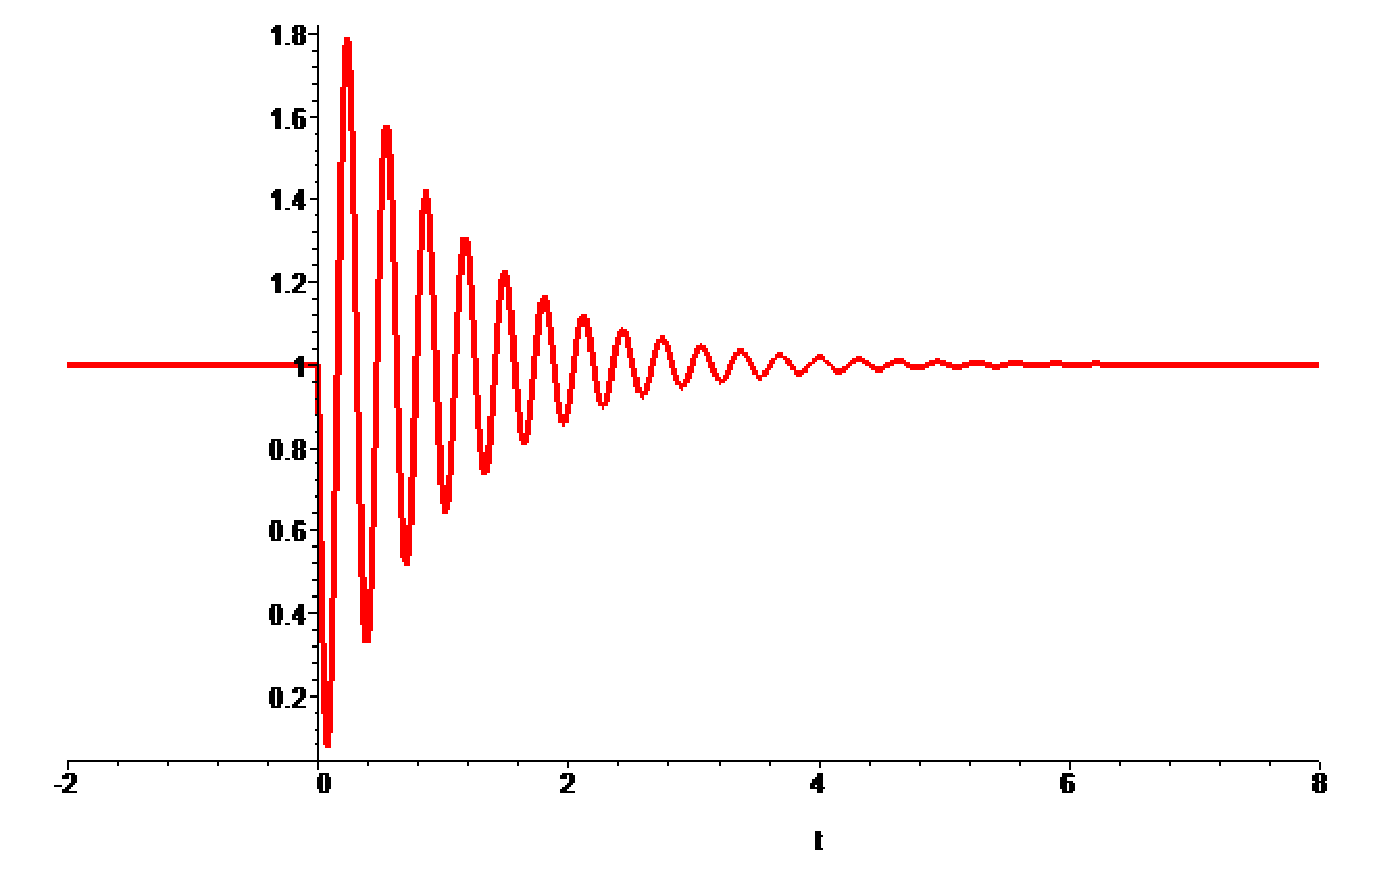
\includegraphics{img/lin_plot.eps}
{\small 
[Figure 4.2.1] A typical linear response signal in time domain}





First we need to calculate the Fourier transform of such signal:





(4.2.2)F[
\mapleinline{inert}{2d}{resp(t);}{%
$\mathrm{resp}(t)$%
}] = 
\mapleinline{inert}{2d}{chi(omega) =
2*(-10-Pi*delta(omega)*omega^2+2*i*Pi*delta(omega)+401*Pi*delta(omega)
)/(omega*i+1-20*i)/(omega*i+1+20*i);}{%
$\chi (\omega )=\frac {2\,( - 10 - \pi \,\delta (\omega )\,\omega
 ^{2} + 2\,i\,\pi \,\delta (\omega ) + 401\,\pi \,\delta (\omega 
))}{(\omega \,i + 1 - 20\,i)\,(\omega \,i + 1 + 20\,i)}$%
} \symbol{126}= 
\mapleinline{inert}{2d}{(-20)/(omega*i+1-20*i)/(omega*i+1+20*i);}{%
$\frac { - 20}{(\omega \,i + 1 - 20\,i)\,(\omega \,i + 1 + 20\,i)
}$%
}, where 
\mapleinline{inert}{2d}{delta(omega);}{%
$\delta (\omega )$%
} - Dirac delta function can be omitted from the numerical point of
view.





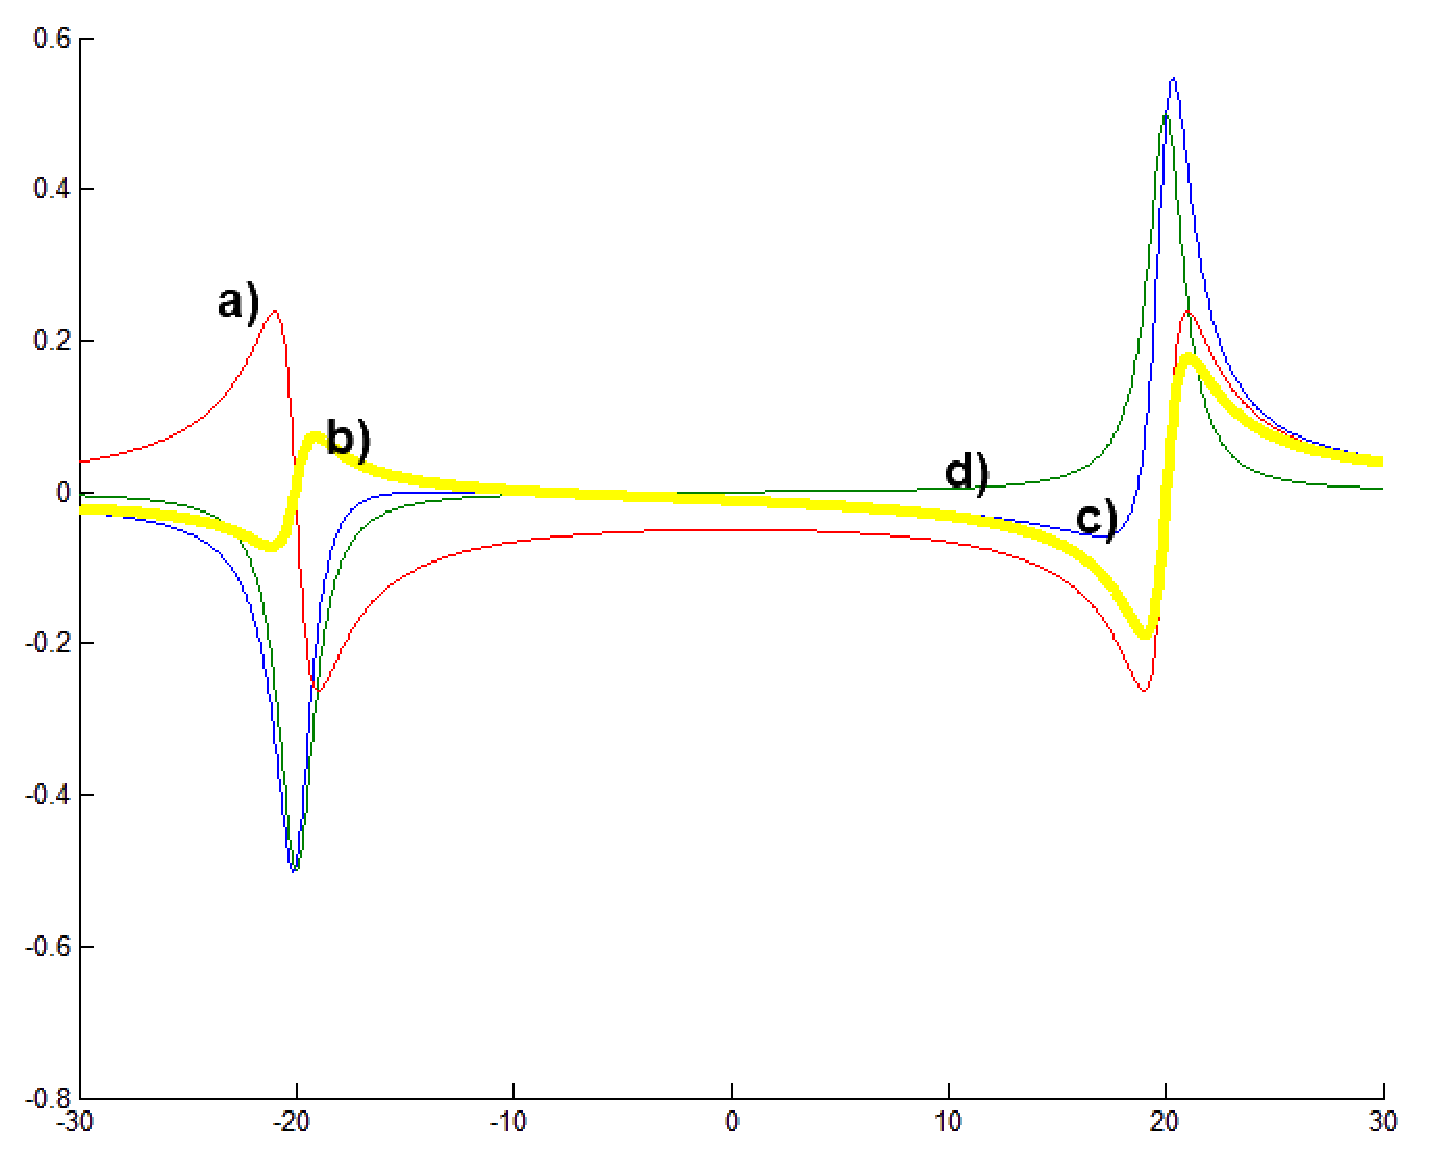
\includegraphics{img/htran_lin.eps}
{\small [Figure 4.2.2] Result plotted together a) The plot of the real
part of 
\mapleinline{inert}{2d}{chi(omega);}{%
$\chi (\omega )$%
}} {\small b) absolute error plot (c-plot minus d-plot) c) imaginary
part of 
\mapleinline{inert}{2d}{chi(omega);}{%
$\chi (\omega )$%
}} {\small obtained with the Hilbert transform of a-plot d) imaginary
part of 
\mapleinline{inert}{2d}{chi(omega);}{%
$\chi (\omega )$%
}}{\small  calculated analytically.}





\textit{Example cases for solving the Kramers-Kronig relations in
linear model using HTRAN - with short conclusions}




\subsection{HTRAN for simple nonlinear model - results}



We get the equation for pump-and-probe susceptibility equation (2.3.1)
and assume some values for the function parameters:





(4.3.1) 
\mapleinline{inert}{2d}{chi[pp](delta) =
G*n[0]*gamma[ba]/(Delta+delta+I*eta)*(1-Omega[1]^2*(Delta-delta+I*eta)
*(delta+2*I*eta)/(Delta-I*eta)/((delta+I*theta)*(Delta+delta+I*eta)*(d
elta-Delta+I*eta)-Omega[1]^2*(delta+I*eta))/2);}{%
${\chi _{\mathit{pp}}}(\delta )=\frac {G\,{n_{0}}\,{\gamma _{
\mathit{ba}}}\, \left(  \! 1 - \frac {{\Omega _{1}}^{2}\,(\Delta 
 - \delta  + I\,\eta )\,(\delta  + 2\,I\,\eta )}{(\Delta  - I\,
\eta )\,((\delta  + I\,\theta )\,(\Delta  + \delta  + I\,\eta )\,
(\delta  - \Delta  + I\,\eta ) - {\Omega _{1}}^{2}\,(\delta  + I
\,\eta ))\,2} \!  \right) }{\Delta  + \delta  + I\,\eta }$%
}     





where:
\mapleinline{inert}{2d}{G = 1;}{%
$G=1$%
}, 
\mapleinline{inert}{2d}{gamma[ba];}{%
${\gamma _{\mathit{ba}}}$%
} = -0.1, 
\mapleinline{inert}{2d}{n[0];}{%
${n_{0}}$%
} = 1, 
\mapleinline{inert}{2d}{Delta = 1.3;}{%
$\Delta =\mbox{1.3}$%
}, 
\mapleinline{inert}{2d}{eta = 1;}{%
$\eta =1$%
}, 
\mapleinline{inert}{2d}{theta = 1.4;}{%
$\theta =\mbox{1.4}$%
}, 
\mapleinline{inert}{2d}{Omega[1] = 4.3;}{%
${\Omega _{1}}=\mbox{4.3}$%
}





The results for such set of arbitrary parameters are shown on the
Figure 4.3.1.





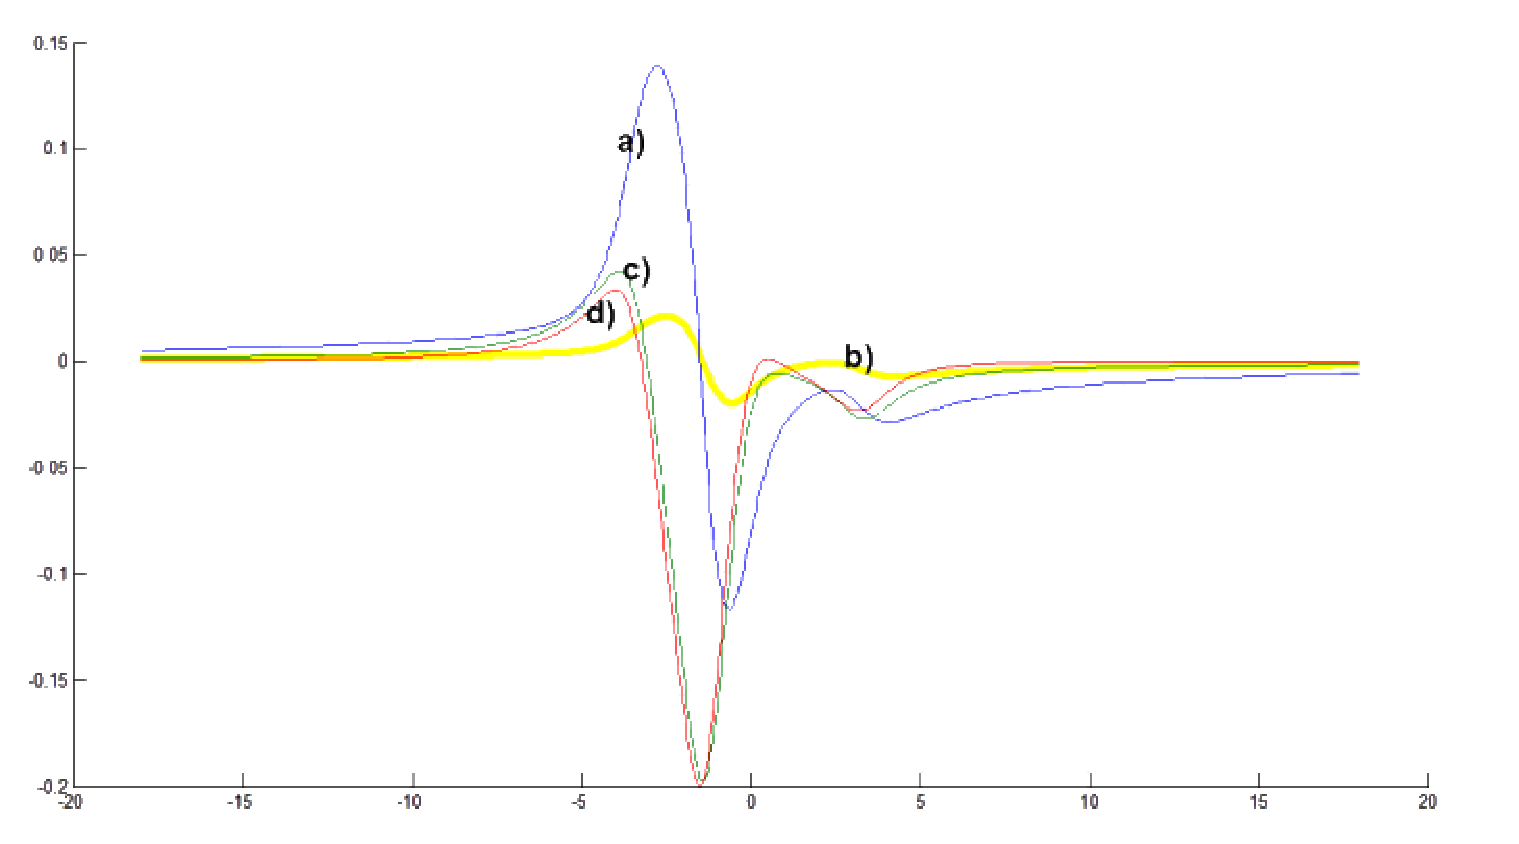
\includegraphics{img/htran_pnp_2d.eps}
{\small [Figure 4.3.1] Result plotted together a) The plot of the real
part of 
\mapleinline{inert}{2d}{chi[pp](delta);}{%
${\chi _{\mathit{pp}}}(\delta )$%
}} {\small b) absolute error plot (c-plot minus d-plot) c) imaginary
part of 
\mapleinline{inert}{2d}{chi[pp](delta);}{%
${\chi _{\mathit{pp}}}(\delta )$%
}} {\small obtained with the Hilbert transform of a-plot d) imaginary
part of 
\mapleinline{inert}{2d}{chi[pp](delta);}{%
${\chi _{\mathit{pp}}}(\delta )$%
}}{\small  calculated analytically.}





The resulted b-plot seems to be a not-so-bad introduction into the
Hilbert transform evaluation, as we have only employed the simple
Simpson's rule. We would also like to perform the 3-Dimensional
analysis of the assumed pump-probe susceptibility, so we employ the
(2.4.5a-b) equations for each frequency, which require performing two
integrations (one, for each frequency-domain argument).
Unfortunatelly, only the obtained 3-Dimensial shapes are similary to
the original ones, but the relative error is huge:





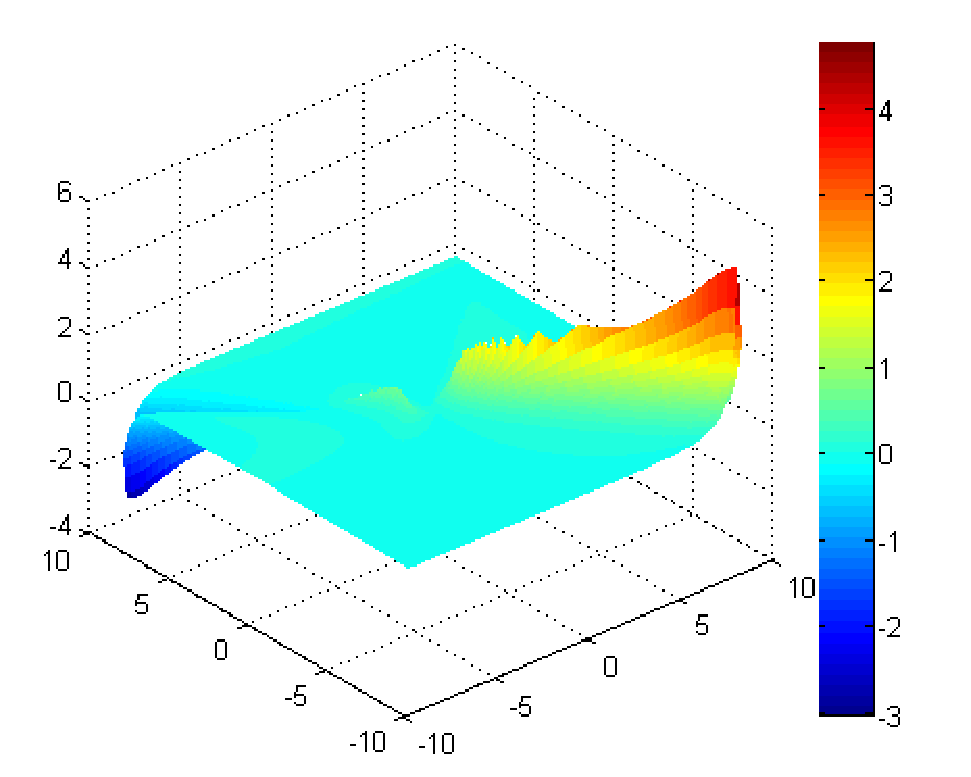
\includegraphics{img/htran_pnp_3derr.eps}
{\small [Figure 4.3.2] Combined relative error of 3-Dimensial calculations.
The light-cyan color shows the area of error below 100\%, which is not
very bad, but there are areas with error more above 100\%.}





Let's now perform the evaluation for the wave-mixing model as stated
in the model described by (2.3.2a). We expand this equation to resolve
the complex conjugate of D function and the resulting function is:





(4.3.3) 
\mapleinline{inert}{2d}{chi[mix](delta) =
2/3*N*w[0]*mu[ba]^4*(-delta-Delta-i/T[2])*(delta+2*i/T[2])/(Delta+i/T[
2])/epsilon0/(h^3)/(Delta+delta+i/T[2])/(delta^3-2*i*delta^2/T[2]-delt
a*Delta^2-2*i/T[1]*delta/T[2]-delta/(T[2]^2)+delta^2/T[1]-Delta^2/T[1]
-1/(T[1]*T[2]^2)-Omega[2]*delta+Omega[2]/T[2]*i);}{%
${\chi _{\mathit{mix}}}(\delta )=2\,N\,{w_{0}}\,{\mu _{\mathit{ba
}}}^{4}\,( - \delta  - \Delta  - \frac {i}{{T_{2}}})\,(\delta  + 
\frac {2\,i}{{T_{2}}}) \left/ {\vrule 
height0.90em width0em depth0.90em} \right. \!  \! (3\,(\Delta  + 
\frac {i}{{T_{2}}})\,\varepsilon 0\,h^{3}\,(\Delta  + \delta  + 
\frac {i}{{T_{2}}})\,(\delta ^{3} - \frac {2\,i\,\delta ^{2}}{{T
_{2}}} - \delta \,\Delta ^{2} - \frac {2\,i\,\delta }{{T_{1}}\,{T
_{2}}} - \frac {\delta }{{T_{2}}^{2}} + \frac {\delta ^{2}}{{T_{1
}}} - \frac {\Delta ^{2}}{{T_{1}}} - \frac {1}{{T_{1}}\,{T_{2}}^{
2}} - {\Omega _{2}}\,\delta  + \frac {{\Omega _{2}}\,i}{{T_{2}}})
)$%
}





With such an complex function we obtain the following two and three
dimensional results:





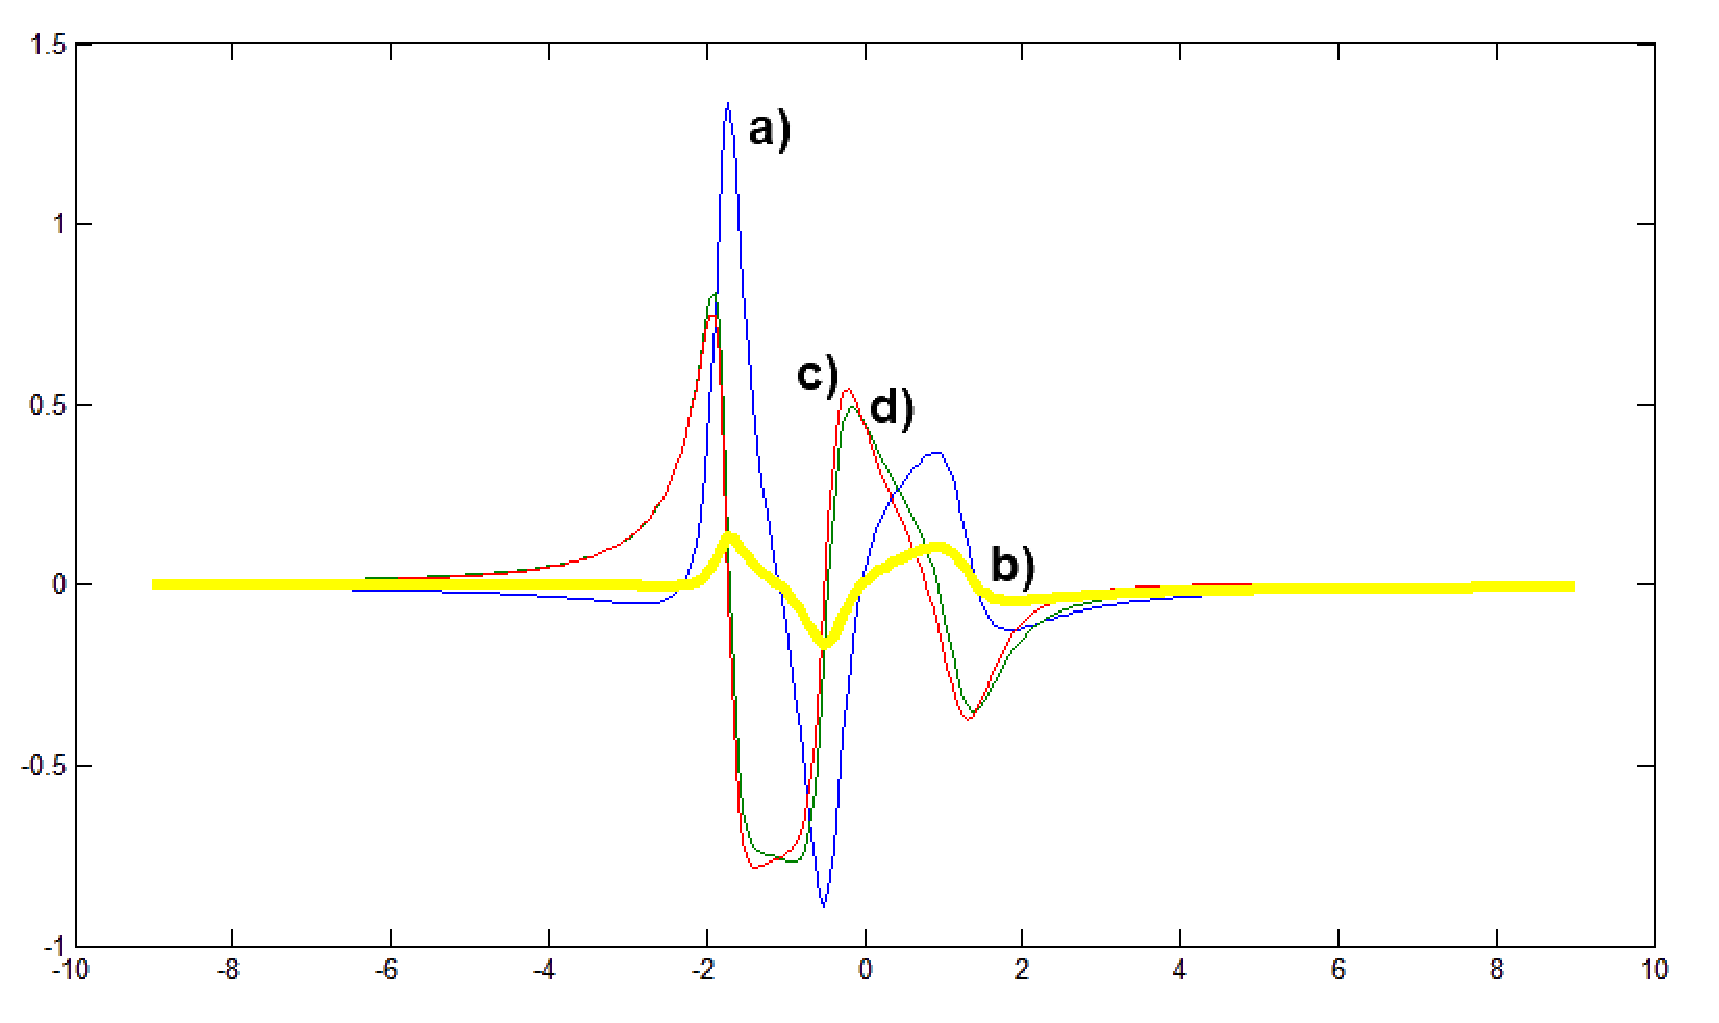
\includegraphics[width=170mm]{img/htran_fmix_2d.eps}
{\small [Figure 4.3.3] Results plotted together a) The plot of the
real part of 
\mapleinline{inert}{2d}{chi[mix](delta);}{%
${\chi _{\mathit{mix}}}(\delta )$%
}} {\small b) absolute error plot (c-plot minus d-plot) c) (red)
imaginary part of 
\mapleinline{inert}{2d}{chi[pp](delta);}{%
${\chi _{\mathit{pp}}}(\delta )$%
}} {\small obtained with the Hilbert transform of a-plot d) (gre
imaginary part of 
\mapleinline{inert}{2d}{chi[pp](delta);}{%
${\chi _{\mathit{pp}}}(\delta )$%
}}{\small  calculated analytically.}





As the obtained 3-Dimensial shape looks very similar to those obtained
analytically, the relative error still remains huge for some areas:





\includegraphics{img/htran_fmix_3derr.eps}
[{\small Figure 4.3.4] Combined relative error for the real part of
nonlinear susceptibility 
\mapleinline{inert}{2d}{chi[mix](delta);}{%
${\chi _{\mathit{mix}}}(\delta )$%
} describing the wave-mixing process.. }





\textit{Example cases for solving the Kramers-Kronig relations in
simple nonlinear model using HTRAN - with short conslusions.}




\subsection{HTRAN for simple quantum-perturbative model -
results}



We will use the models already prepared for both linear and
second-order nonlinear susceptibilities defined in Chapter 2.5. 





(4.4.1) 
\mapleinline{inert}{2d}{chi[1,qp](omega);}{%
${\chi _{1, \,\mathit{qp}}}(\omega )$%
} = 
\mapleinline{inert}{2d}{sum(mu[1,n]*mu[2,n]/(Omega[n]-omega-i*gamma[n])+mu[2,n]*mu[1,n]/(Omeg
a[n]+omega+i*gamma[n]),n = 1 .. 2)*N/epsilon0/h;}{%
$\frac { \left(  \! \sum _{n=1}^{2}\,(\frac {{\mu _{1, \,n}}\,{
\mu _{2, \,n}}}{{\Omega _{n}} - \omega  - i\,{\gamma _{n}}} + 
\frac {{\mu _{2, \,n}}\,{\mu _{1, \,n}}}{{\Omega _{n}} + \omega 
 + i\,{\gamma _{n}}}) \!  \right) \,N}{\varepsilon 0\,h}$%
}





where:
\mapleinline{inert}{2d}{mu;}{%
$\mu $%
} = 
\mapleinline{inert}{2d}{[[1, 3], [-1, -2]];}{%
$[[1, \,3], \,[ - 1, \, - 2]]$%
}, 
\mapleinline{inert}{2d}{Omega = [3, 16];}{%
$\Omega =[3, \,16]$%
}, 
\mapleinline{inert}{2d}{gamma = [1, 2];}{%
$\gamma =[1, \,2]$%
}, 
\mapleinline{inert}{2d}{N = 5;}{%
$N=5$%
}, 
\mapleinline{inert}{2d}{epsilon[0] = 1,h = -1;}{%
${\varepsilon _{0}}=1, \,h= - 1$%
}





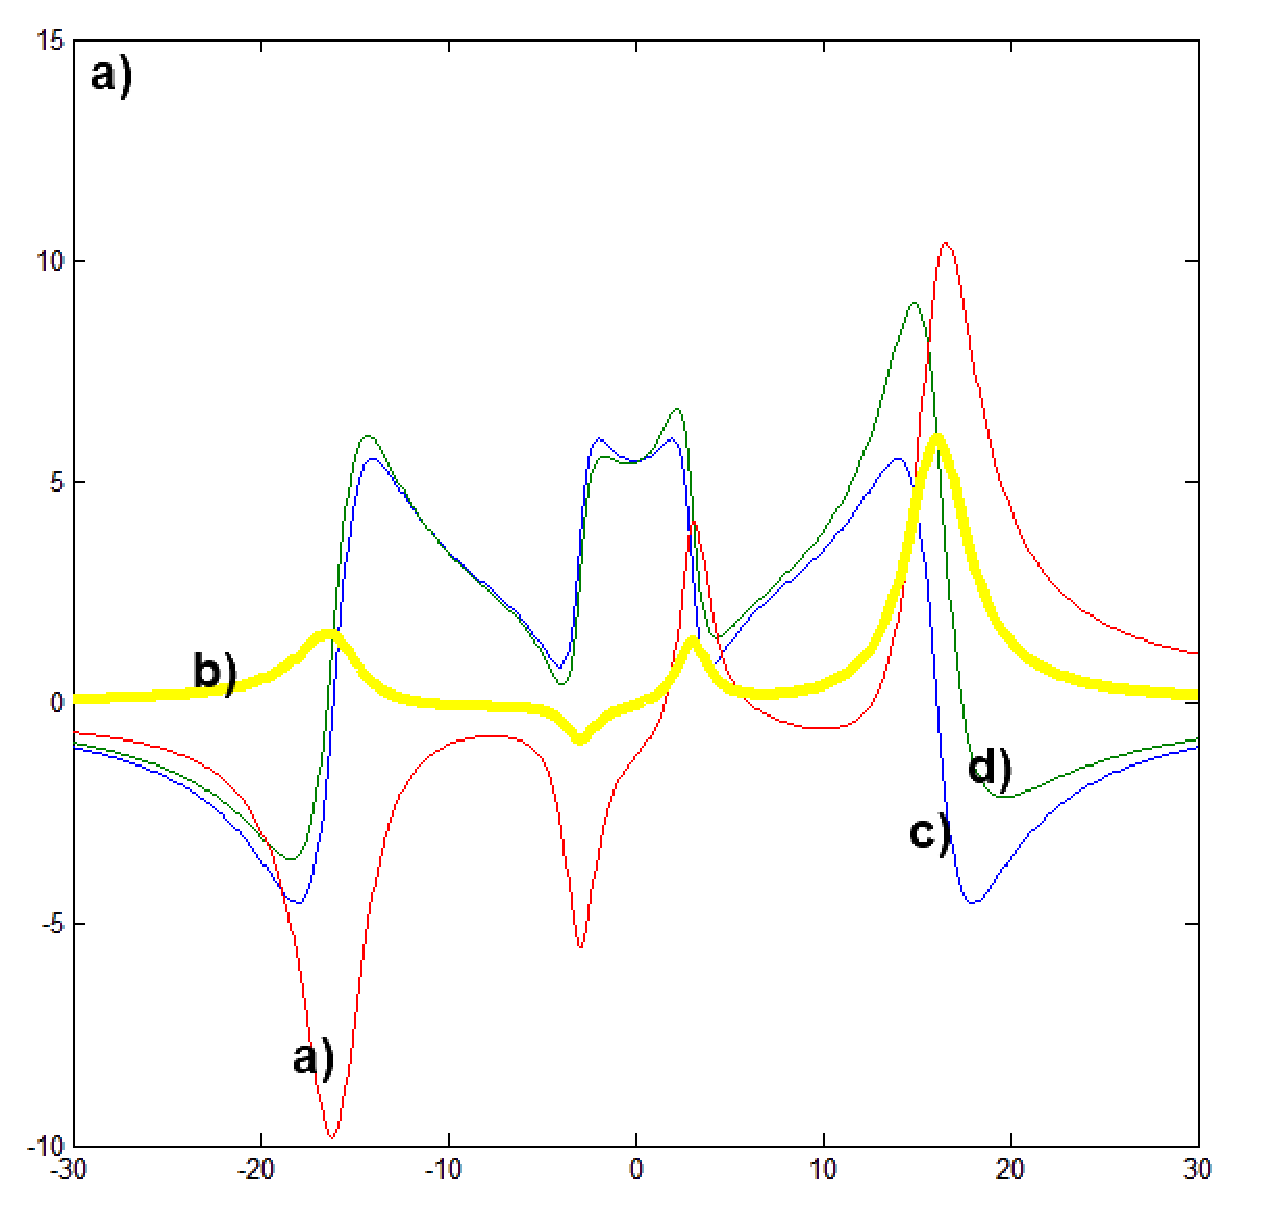
\includegraphics[width=170mm]{img/htran_qp_2da.eps}
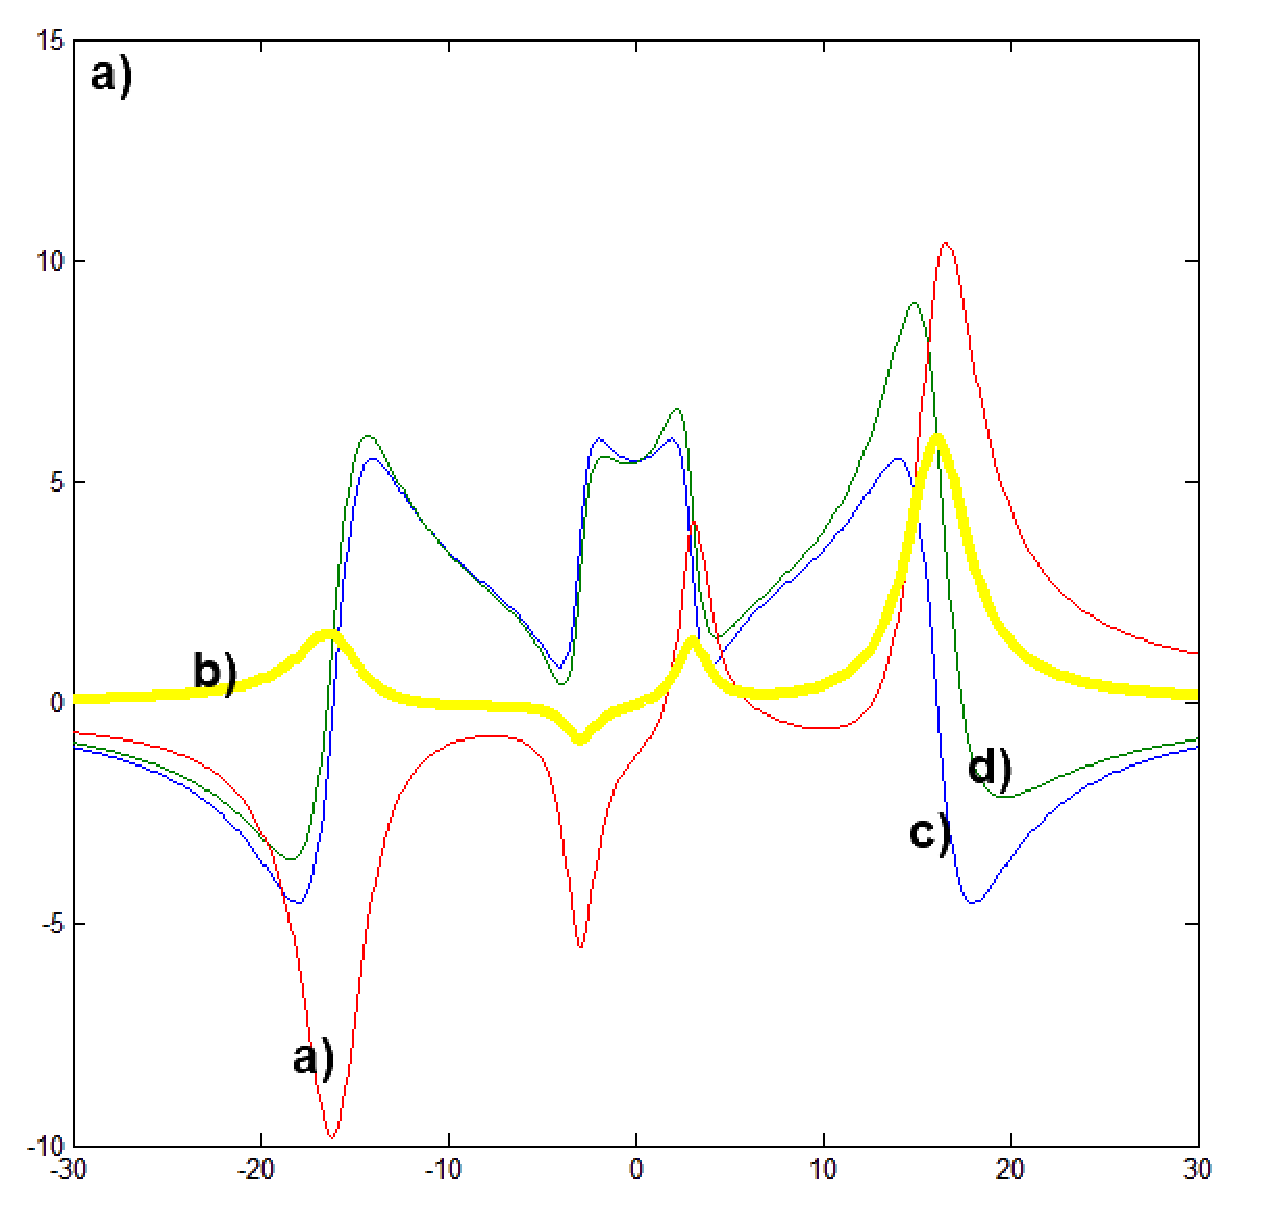
\includegraphics[width=170mm]{img/htran_qp_2da.eps}
{\small [Figures 4.4.1a-b] Result plotted together 
[4.4.1.a] a) The plot of the imag part of 
\mapleinline{inert}{2d}{chi[1,qp](delta);}{%
${\chi _{1, \,\mathit{qp}}}(\delta )$%
}} {\small b) absolute error plot (d-plot minus c-plot) c) real part
of 
\mapleinline{inert}{2d}{chi[pp](delta);}{%
${\chi _{\mathit{pp}}}(\delta )$%
}}{\small  calculated analytically d) real part of 
\mapleinline{inert}{2d}{chi[1,qp](delta);}{%
${\chi _{1, \,\mathit{qp}}}(\delta )$%
}} {\small obtained with the Hilbert transform of a-plot
[4.4.1.b] a) The plot of the real part of 
\mapleinline{inert}{2d}{chi[1,qp](delta);}{%
${\chi _{1, \,\mathit{qp}}}(\delta )$%
}} {\small b) absolute error plot (d-plot minus c-plot) c) imaginary
part of 
\mapleinline{inert}{2d}{chi[pp](delta);}{%
${\chi _{\mathit{pp}}}(\delta )$%
}}{\small  calculated analytically d) imaginary part of 
\mapleinline{inert}{2d}{chi[1,qp](delta);}{%
${\chi _{1, \,\mathit{qp}}}(\delta )$%
}} {\small obtained with the Hilbert transform of a-plot }





(4.4.2) 
\mapleinline{inert}{2d}{chi[2, qp](omega[1],omega[2]) =
N/2/epsilon[0]/(h^2)*sum(sum(sum(mu[l,n]*mu[nm]*mu[ml]/(Omega[nl]-omeg
a1-omega2-i*gamma[nl])/(Omega[ml]-omega1-i*gamma[ml])+mu[l,n]*mu[nm]*m
u[ml]/(Omega[nl]-omega1-omega1-i*gamma[nl])/(Omega[ml]-omega2-i*gamma[
ml])+mu[l,n]*mu[nm]*mu[ml]/(Omega[mn]-omega1-omega2-i*gamma[mn])/(Omeg
a[nl]+omega2+i*gamma[nl])+mu[l,n]*mu[nm]*mu[ml]/(Omega[mn]-omega1-omeg
a2-i*gamma[mn])/(Omega[nl]+omega2+i*gamma[nl])+mu[l,n]*mu[nm]*mu[ml]/(
Omega[nm]+omega1+omega2+i*gamma[nm])/(Omega[ml]-omega1-i*gamma[ml])+mu
[l,n]*mu[nm]*mu[ml]/(Omega[nm]+omega1+omega2+i*gamma[nm])/(Omega[ml]-o
mega1-i*gamma[ml])+mu[l,n]*mu[nm]*mu[ml]/(Omega[ml]+omega1+omega2+i*ga
mma[ml])/(Omega[nl]+omega1+i*gamma[nl])+mu[l,n]*mu[nm]*mu[ml]/(Omega[m
l]+omega1+omega2+i*gamma[ml])/(Omega[nl]+omega2+i*gamma[nl]),l = 1 ..
2),m = 1 .. 2),n = 1 .. 2);}{%
${\chi _{2, \,\mathit{qp}}}({\omega _{1}}, \,{\omega _{2}})=N\,
 \left(  \! \sum _{n=1}^{2}\, \left(  \! \sum _{m=1}^{2}\,
 \left(  \! \sum _{l=1}^{2}\,(\frac {{\mu _{l, \,n}}\,{\mu _{
\mathit{nm}}}\,{\mu _{\mathit{ml}}}}{({\Omega _{\mathit{nl}}} - 
\omega 1 - \omega 2 - i\,{\gamma _{\mathit{nl}}})\,({\Omega _{
\mathit{ml}}} - \omega 1 - i\,{\gamma _{\mathit{ml}}})} + \frac {
{\mu _{l, \,n}}\,{\mu _{\mathit{nm}}}\,{\mu _{\mathit{ml}}}}{({
\Omega _{\mathit{nl}}} - \omega 1 - \omega 1 - i\,{\gamma _{
\mathit{nl}}})\,({\Omega _{\mathit{ml}}} - \omega 2 - i\,{\gamma 
_{\mathit{ml}}})} + \frac {{\mu _{l, \,n}}\,{\mu _{\mathit{nm}}}
\,{\mu _{\mathit{ml}}}}{({\Omega _{\mathit{mn}}} - \omega 1 - 
\omega 2 - i\,{\gamma _{\mathit{mn}}})\,({\Omega _{\mathit{nl}}}
 + \omega 2 + i\,{\gamma _{\mathit{nl}}})} + \frac {{\mu _{l, \,n
}}\,{\mu _{\mathit{nm}}}\,{\mu _{\mathit{ml}}}}{({\Omega _{
\mathit{mn}}} - \omega 1 - \omega 2 - i\,{\gamma _{\mathit{mn}}})
\,({\Omega _{\mathit{nl}}} + \omega 2 + i\,{\gamma _{\mathit{nl}}
})} + \frac {{\mu _{l, \,n}}\,{\mu _{\mathit{nm}}}\,{\mu _{
\mathit{ml}}}}{({\Omega _{\mathit{nm}}} + \omega 1 + \omega 2 + i
\,{\gamma _{\mathit{nm}}})\,({\Omega _{\mathit{ml}}} - \omega 1
 - i\,{\gamma _{\mathit{ml}}})} + \frac {{\mu _{l, \,n}}\,{\mu _{
\mathit{nm}}}\,{\mu _{\mathit{ml}}}}{({\Omega _{\mathit{nm}}} + 
\omega 1 + \omega 2 + i\,{\gamma _{\mathit{nm}}})\,({\Omega _{
\mathit{ml}}} - \omega 1 - i\,{\gamma _{\mathit{ml}}})} + \frac {
{\mu _{l, \,n}}\,{\mu _{\mathit{nm}}}\,{\mu _{\mathit{ml}}}}{({
\Omega _{\mathit{ml}}} + \omega 1 + \omega 2 + i\,{\gamma _{
\mathit{ml}}})\,({\Omega _{\mathit{nl}}} + \omega 1 + i\,{\gamma 
_{\mathit{nl}}})} + \frac {{\mu _{l, \,n}}\,{\mu _{\mathit{nm}}}
\,{\mu _{\mathit{ml}}}}{({\Omega _{\mathit{ml}}} + \omega 1 + 
\omega 2 + i\,{\gamma _{\mathit{ml}}})\,({\Omega _{\mathit{nl}}}
 + \omega 2 + i\,{\gamma _{\mathit{nl}}})}) \!  \right)  \! 
 \right)  \!  \right)  \left/ {\vrule 
height0.47em width0em depth0.47em} \right. \!  \! (2\,{
\varepsilon _{0}}\,h^{2})$%
}





where:
\mapleinline{inert}{2d}{mu;}{%
$\mu $%
} = 
\mapleinline{inert}{2d}{[[1, 3], [-1, -2]];}{%
$[[1, \,3], \,[ - 1, \, - 2]]$%
}, 
\mapleinline{inert}{2d}{Omega = [[3, 16], [4, 12]];}{%
$\Omega =[[3, \,16], \,[4, \,12]]$%
}, 
\mapleinline{inert}{2d}{gamma = [[1, 2], [-1, 3]];}{%
$\gamma =[[1, \,2], \,[ - 1, \,3]]$%
}, 
\mapleinline{inert}{2d}{N = 5;}{%
$N=5$%
}, 
\mapleinline{inert}{2d}{epsilon[0] = 1,h = -1;}{%
${\varepsilon _{0}}=1, \,h= - 1$%
}





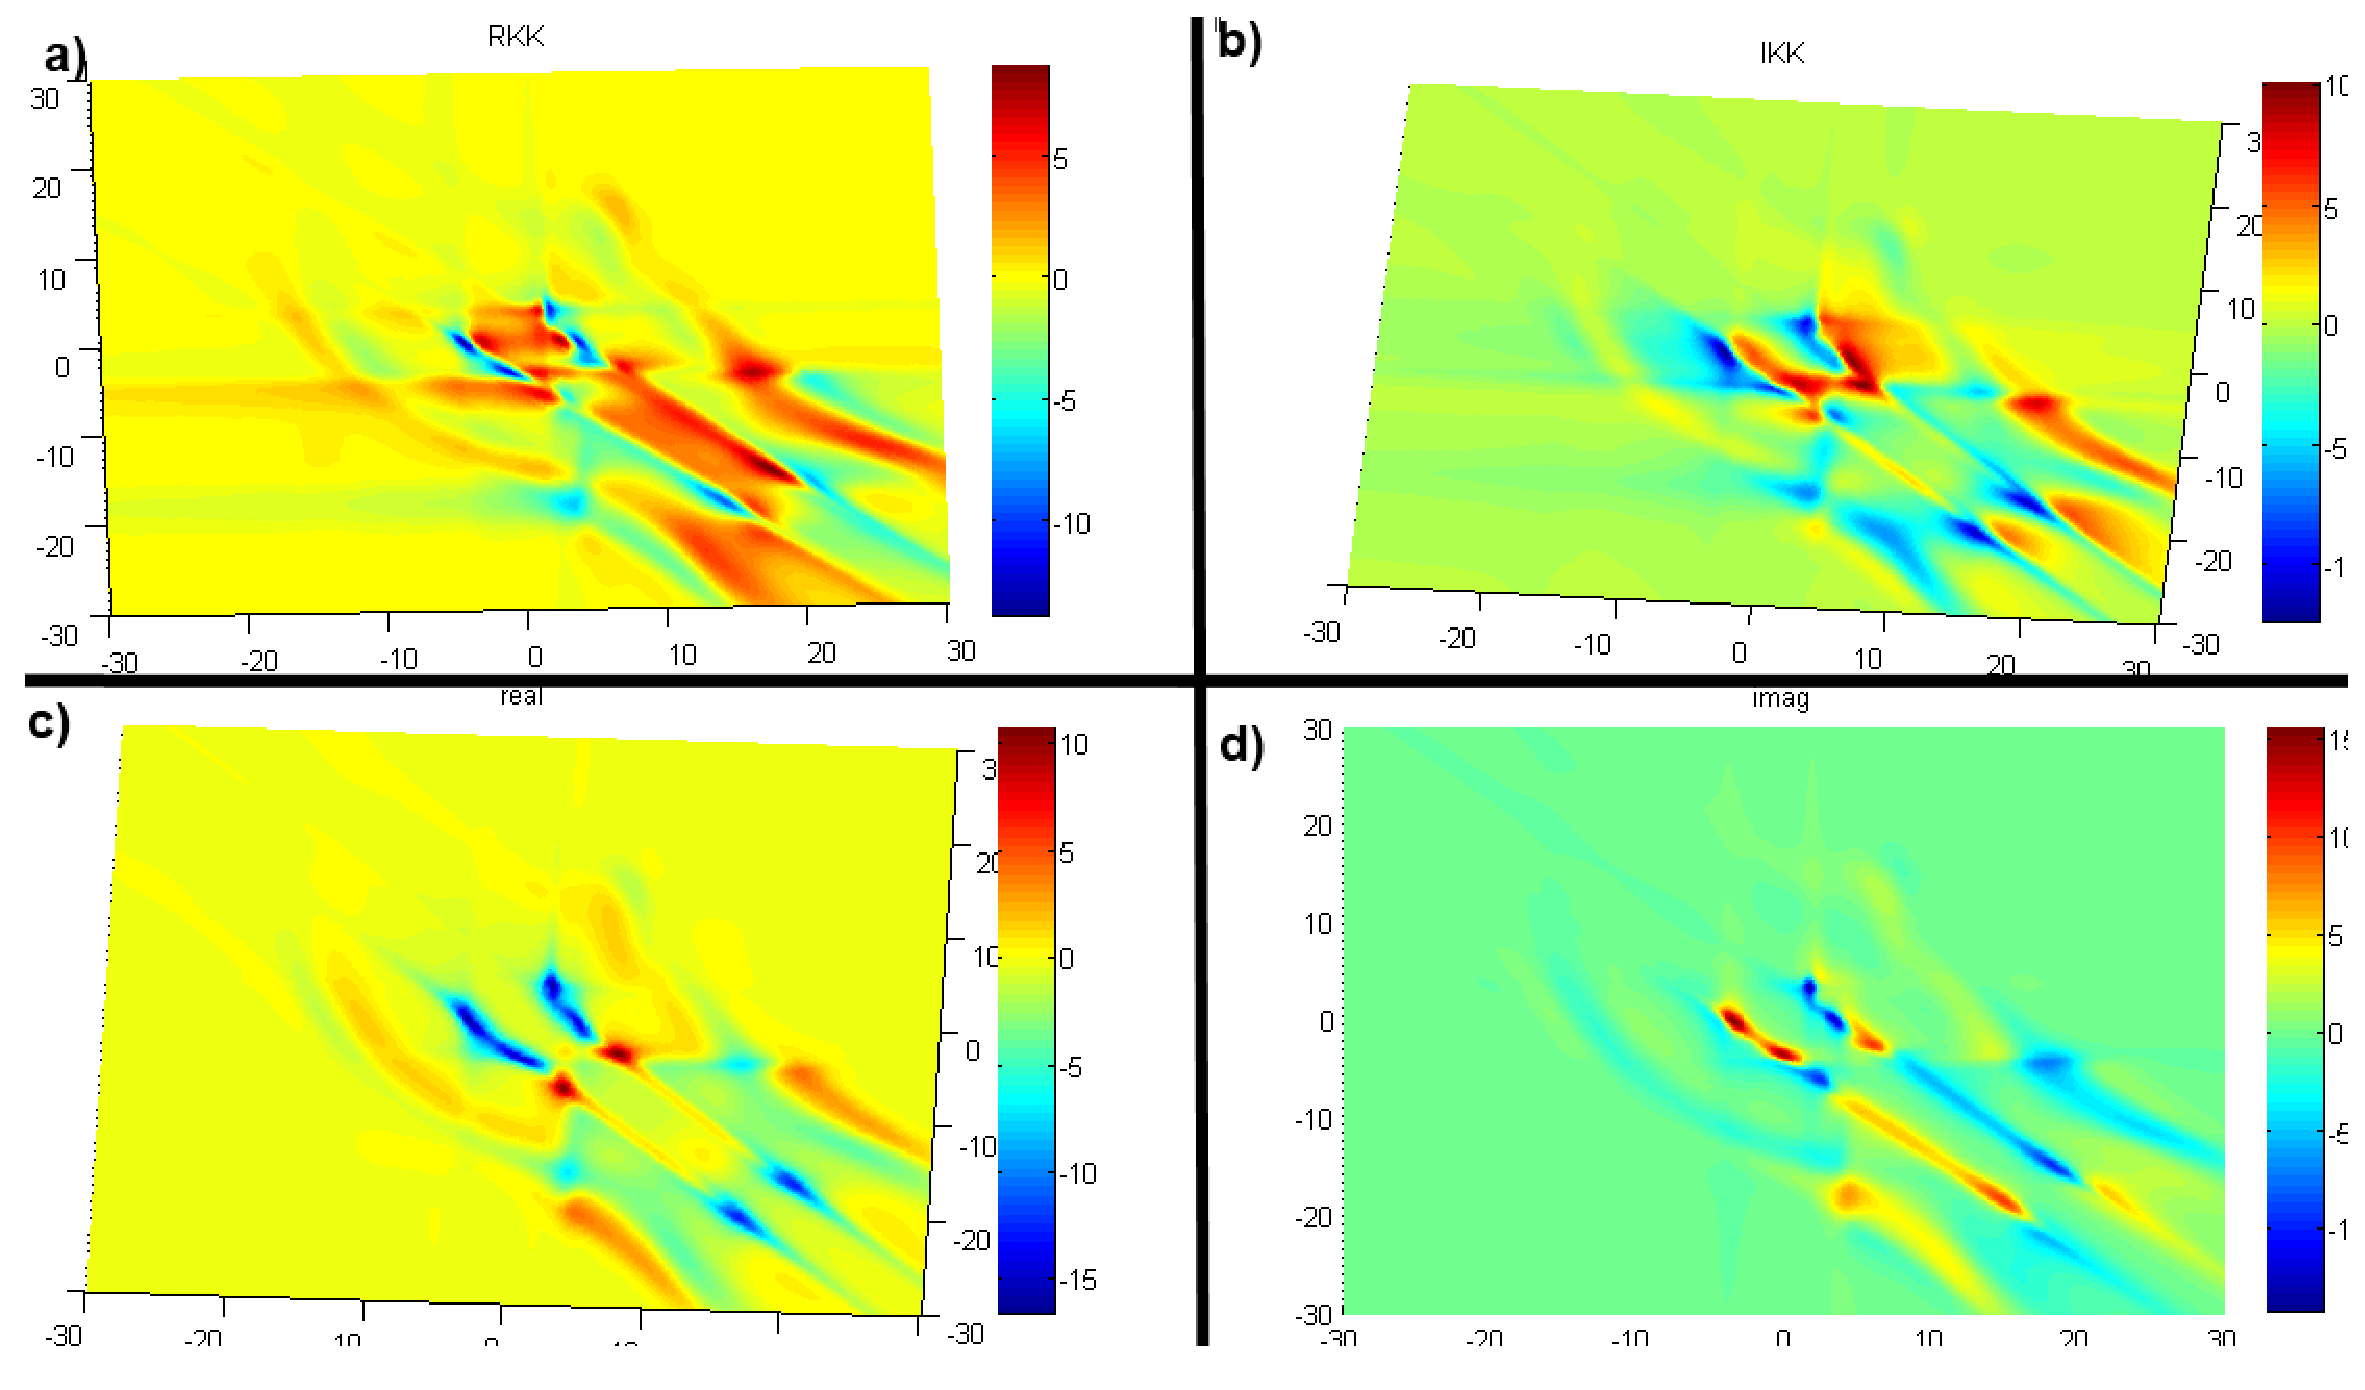
\includegraphics[width=170mm]{img/htran_qp_3d.eps}
{\small 
[Figures 4.4.2a-d] Results of the HTRAN 3-Dimensional method plotted
together.  a) - The calculated real part of 
\mapleinline{inert}{2d}{chi[2,qp];}{%
${\chi _{2, \,\mathit{qp}}}$%
} b) The calculated imaginary part of 
\mapleinline{inert}{2d}{chi[2,qp];}{%
${\chi _{2, \,\mathit{qp}}}$%
} c) The real part of nonlinear susceptibility 
\mapleinline{inert}{2d}{chi[2,qp];}{%
${\chi _{2, \,\mathit{qp}}}$%
} calculated analytically d) The imaginary part of the nonlinear
susceptibility 
\mapleinline{inert}{2d}{chi[2,qp];}{%
${\chi _{2, \,\mathit{qp}}}$%
}}





We can see, there is a similarity in obtained plots, but both the
relative and absolute error do not satisfy us at all. Results obtained
with 2-Dimensional model were more satysfying.





Example cases for solving the Kramers-Kronig relations in simple
\textit{quantum-}perturbative model using HTRAN - with short
conslusions.




\subsection{HTRAN for other models - results}



Unfortunatelly the results obtained for the equation (2.8.1) were far
from accurate, so we will not show them for HTRAN method.





\textit{Example cases for solving the Kramers-Kronig relations for
other models using HTRAN - with short conslusions.}




\section{Newton-Cotes quadrature (solving)}

\subsection{Overview of the NC quadrature of arbitrary degree}



Newton-Cotes formula for numerical integration is taken into
consideration. We compare formula for an arbitrary degree - having in
our mind, that the choice between formulas of high and low degree must
be undertaken with the awareness of numerical errors that may arise.
Newton-Cotes quadrature is a method for numerical integration with
equispaced vertices. As we would like to integrate function f = f(x)
within the range 
\mapleinline{inert}{2d}{a .. b;}{%
$a .. b$%
} we introduce the following calculations





(5.1.1a) 
\mapleinline{inert}{2d}{x[n,k] = a+(b-a)/n*k;}{%
${x_{n, \,k}}=a + \frac {(b - a)\,k}{n}$%
}            for 
\mapleinline{inert}{2d}{k = 0,1 .. n;}{%
$k=0, \,1 .. n$%
}
(5.1.1b) 
\mapleinline{inert}{2d}{omega[n](x) = (x-x[n,0])(x-x[n,1])*((NULL) .. (NULL))*(x-x[n,n]);}{%
${\omega _{n}}(x)=(x - {x_{n, \,0}})(x - {x_{n, \,1}})\,(\mathit{
NULL} .. \mathit{NULL})\,(x - {x_{n, \,n}})$%
}
(5.1.1c) 
\mapleinline{inert}{2d}{lambda[n,k](x) =
omega[n](x)/(diff(omega[n](x[n,k]),x)*(x-x[n,k]));}{%
${\lambda _{n, \,k}}(x)=\frac {{\omega _{n}}(x)}{({\frac {
\partial }{\partial x}}\,{\omega _{n}}({x_{n, \,k}}))\,(x - {x_{n
, \,k}})}$%
}        for  
\mapleinline{inert}{2d}{k = 0,1 .. n;}{%
$k=0, \,1 .. n$%
}
(5.1.1d) 
\mapleinline{inert}{2d}{A[n,k] = Int(lambda[n,k](x),x = a .. b);}{%
${A_{n, \,k}}=\int _{a}^{b}{\lambda _{n, \,k}}(x)\,dx$%
} = 
\mapleinline{inert}{2d}{(b-a)/n*(-1)^(n-k)/k!/(n-k)!*int(product(t-j,j = (0, j <> k) .. n),t
= 0 .. n);}{%
$\frac {(b - a)\,( - 1)^{(n - k)}\,\int _{0}^{n}\prod _{j=0, \,j
\neq k}^{n}\,(t - j)\,dt}{n\,k\mathrm{!}\,(n - k)\mathrm{!}}$%
}    for  
\mapleinline{inert}{2d}{k = 0,1 .. n;}{%
$k=0, \,1 .. n$%
}





With such defined parameters the quadrature in sense of Newton-Cotes
is defined as following:





(5.1.2) 
\mapleinline{inert}{2d}{NC[n](f) = A[n,k]*sum(a+k*(b-a)/n,k = 0 .. n);}{%
${\mathit{NC}_{n}}(f)={A_{n, \,k}}\, \left(  \! \sum _{k=0}^{n}\,
(a + \frac {k\,(b - a)}{n}) \!  \right) $%
}





The numerical algorithm for the Newton-Cotes quadrature of an
arbitrary degree has been prepared in Appendix A.2. It has been
modified to omit the singularity and to estimate the number of
mini-steps needed to partition the integration range - see the source
code and comments. The function parameters are defined below:




\subsubsection*{Input arguments: }



fun - the real-valued function we will like to integrate
(function-handle), mandatory argument
a - integration starting point, mandatory argument
b - integration ending point, mandatory argument
tol - required tolerance, default value 
\mapleinline{inert}{2d}{10^(-5);}{%
$10^{( - 5)}$%
}
n - degree of the Newton-Cotes quadrature, default value 8
cs - how close (in absolute value) we would like to get near the
singularity, default value 
\mapleinline{inert}{2d}{10^(-2);}{%
$10^{( - 2)}$%
}
pts - number of points in which user would like to perform the Hilbert
transform, default value 200




\subsubsection*{Output arguments:}



F - an array of points, abscissas



H - calculated Hilbert transform values, ordinates





\textit{The description of the Newton-Cotes algorithm}




\subsection{NC for simple linear model - results}



As the prepared numeric method depends on many input parameter
arguments, we have tried to perform the evaluation in many different
cases, some of those results are stated below. We are calculating the
same model as in 4.2





(5.2.1) 
\mapleinline{inert}{2d}{chi(omega);}{%
$\chi (\omega )$%
} \symbol{126}= 
\mapleinline{inert}{2d}{(-20)/(omega*i+1-20*i)/(omega*i+1+20*i);}{%
$\frac { - 20}{(\omega \,i + 1 - 20\,i)\,(\omega \,i + 1 + 20\,i)
}$%
}








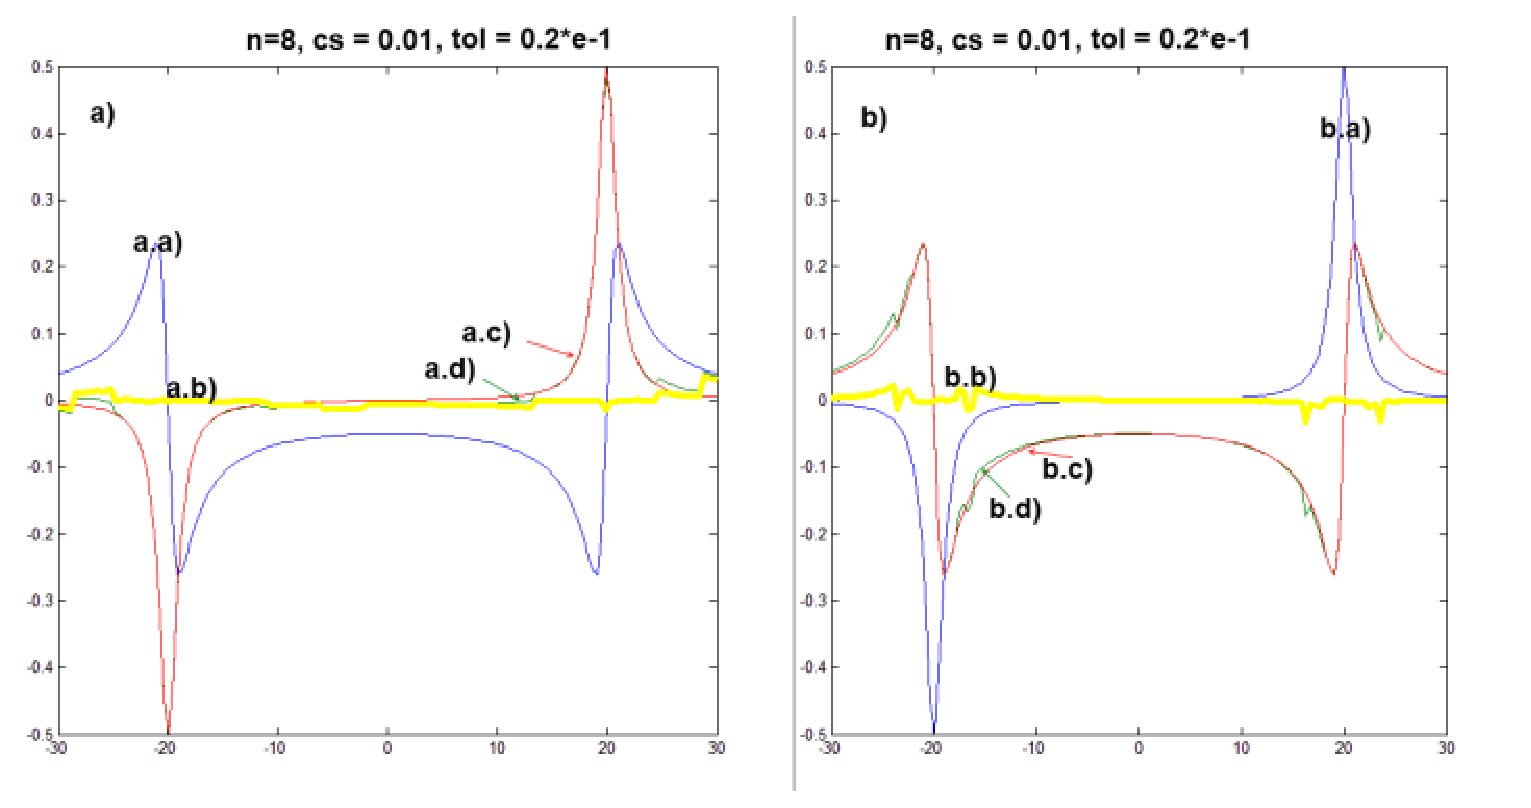
\includegraphics{img/nc_lin1.eps}
[Figure 5.2.1a-b] Calcuations for parameters (
\mapleinline{inert}{2d}{n = 8,cs = .1e-1,tol = .2e-1;}{%
$n=8, \,\mathit{cs}=\mbox{.1e-1}, \,\mathit{tol}=\mbox{.2e-1}$%
} a.a) The plot of the real part of 
\mapleinline{inert}{2d}{chi(omega);}{%
$\chi (\omega )$%
} a.b) absolute error plot (a.d-plot minus a.c-plot) a.c) imaginary
part of 
\mapleinline{inert}{2d}{chi(omega);}{%
$\chi (\omega )$%
} calculated analytically a.d) imaginary part of 
\mapleinline{inert}{2d}{chi(omega);}{%
$\chi (\omega )$%
} obtained with the Hilbert transform of a.a-plot, b.a) The plot of
the imaginary part of 
\mapleinline{inert}{2d}{chi(omega);}{%
$\chi (\omega )$%
} b.b) absolute error plot (b.d-plot minus b.c-plot) b.c) real part of

\mapleinline{inert}{2d}{chi(omega);}{%
$\chi (\omega )$%
} calculated analytically b.d) real part of 
\mapleinline{inert}{2d}{chi(omega);}{%
$\chi (\omega )$%
} obtained with the Hilbert transform of b.a-plot 








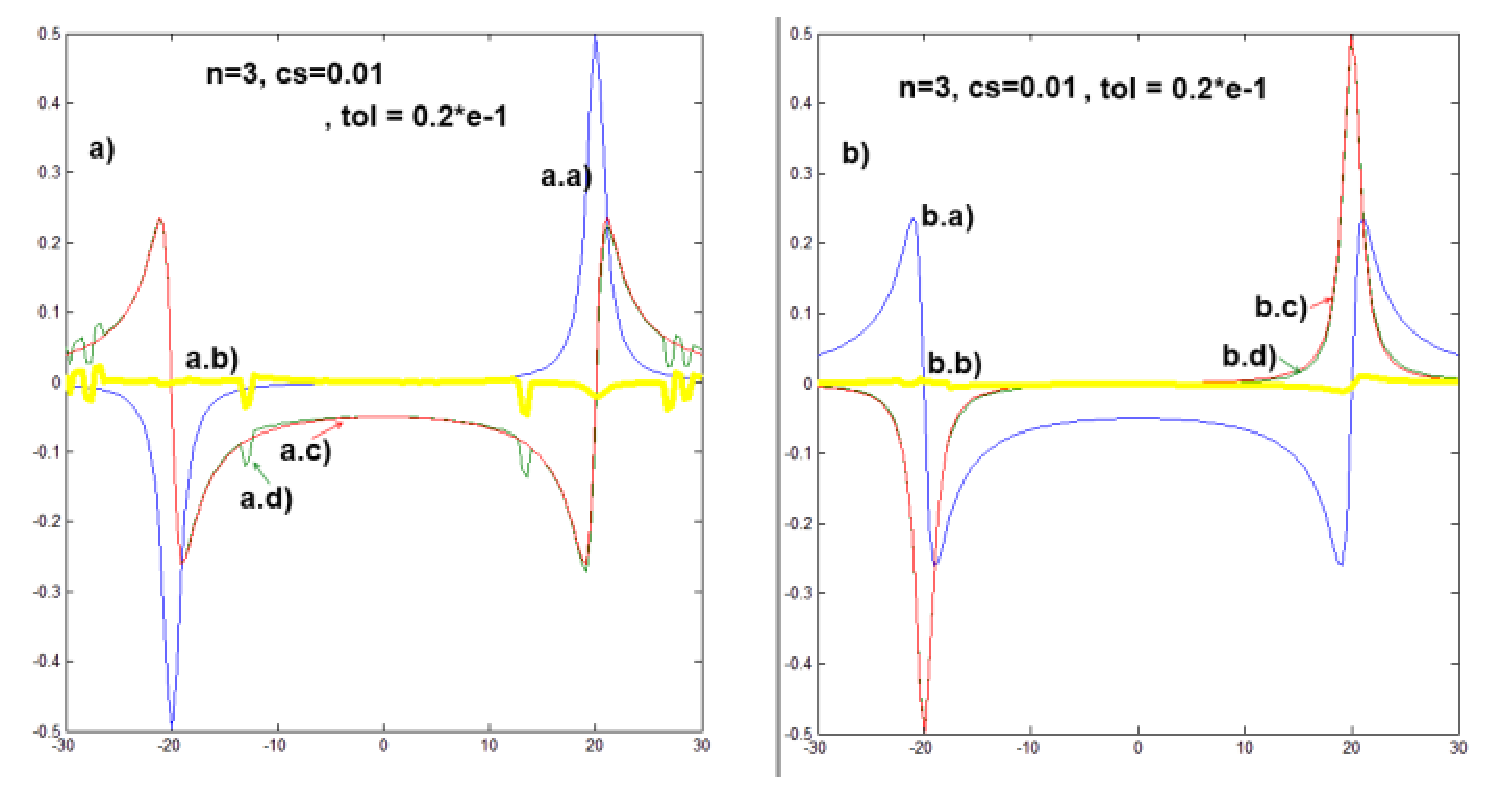
\includegraphics{img/nc_lin2.eps}
[Figure 5.2.2a-b] Calcuations for parameters (
\mapleinline{inert}{2d}{n = 3,cs = .1e-1,tol = .2e-1;}{%
$n=3, \,\mathit{cs}=\mbox{.1e-1}, \,\mathit{tol}=\mbox{.2e-1}$%
}) a.a) The plot of the imaginary part of 
\mapleinline{inert}{2d}{chi(omega);}{%
$\chi (\omega )$%
} a.b) absolute error plot (a.d-plot minus a.c-plot) a.c) real part of

\mapleinline{inert}{2d}{chi(omega);}{%
$\chi (\omega )$%
} calculated analytically a.d) real part of 
\mapleinline{inert}{2d}{chi(omega);}{%
$\chi (\omega )$%
} obtained with the Hilbert transform of a.a-plot, b.a) The plot of
the real part of 
\mapleinline{inert}{2d}{chi(omega);}{%
$\chi (\omega )$%
} b.b) absolute error plot (b.d-plot minus b.c-plot) b.c) imaginary
part of 
\mapleinline{inert}{2d}{chi(omega);}{%
$\chi (\omega )$%
} calculated analytically b.d) imaginary part of 
\mapleinline{inert}{2d}{chi(omega);}{%
$\chi (\omega )$%
} obtained with the Hilbert transform of b.a-plot 








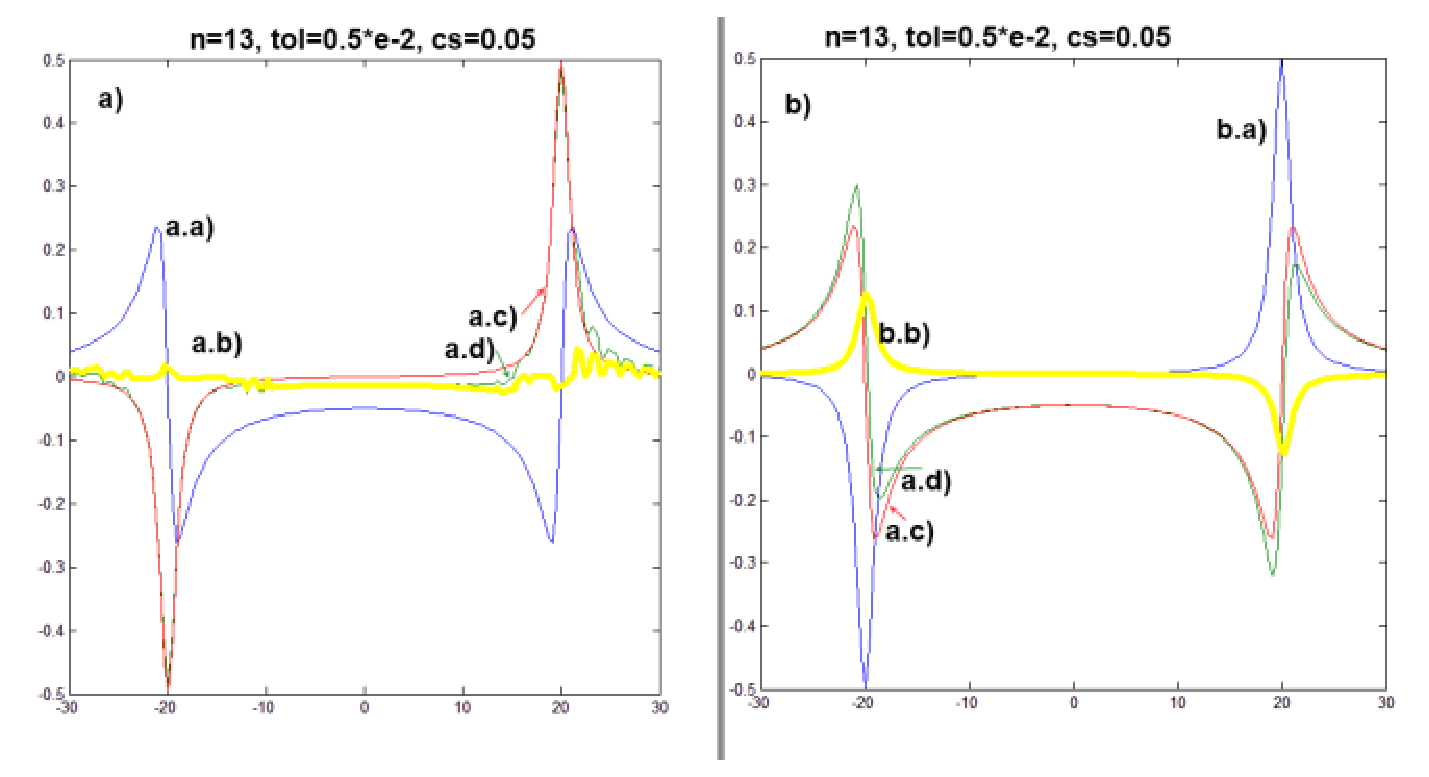
\includegraphics{img/nc_lin3.eps}
[Figure 5.2.3a-b] Calcuations for parameters (
\mapleinline{inert}{2d}{n = 13,tol = .5e-2,cs = .5e-1;}{%
$n=13, \,\mathit{tol}=\mbox{.5e-2}, \,\mathit{cs}=\mbox{.5e-1}$%
}) a.a) The plot of the real part of 
\mapleinline{inert}{2d}{chi(omega);}{%
$\chi (\omega )$%
} a.b) absolute error plot (a.d-plot minus a.c-plot) a.c) imaginary
part of 
\mapleinline{inert}{2d}{chi(omega);}{%
$\chi (\omega )$%
} calculated analytically a.d) imaginary part of 
\mapleinline{inert}{2d}{chi(omega);}{%
$\chi (\omega )$%
} obtained with the Hilbert transform of a.a-plot, b.a) The plot of
the imaginary part of 
\mapleinline{inert}{2d}{chi(omega);}{%
$\chi (\omega )$%
} b.b) absolute error plot (b.d-plot minus b.c-plot) b.c) real part of

\mapleinline{inert}{2d}{chi(omega);}{%
$\chi (\omega )$%
} calculated analytically b.d) real part of 
\mapleinline{inert}{2d}{chi(omega);}{%
$\chi (\omega )$%
} obtained with the Hilbert transform of b.a-plot 








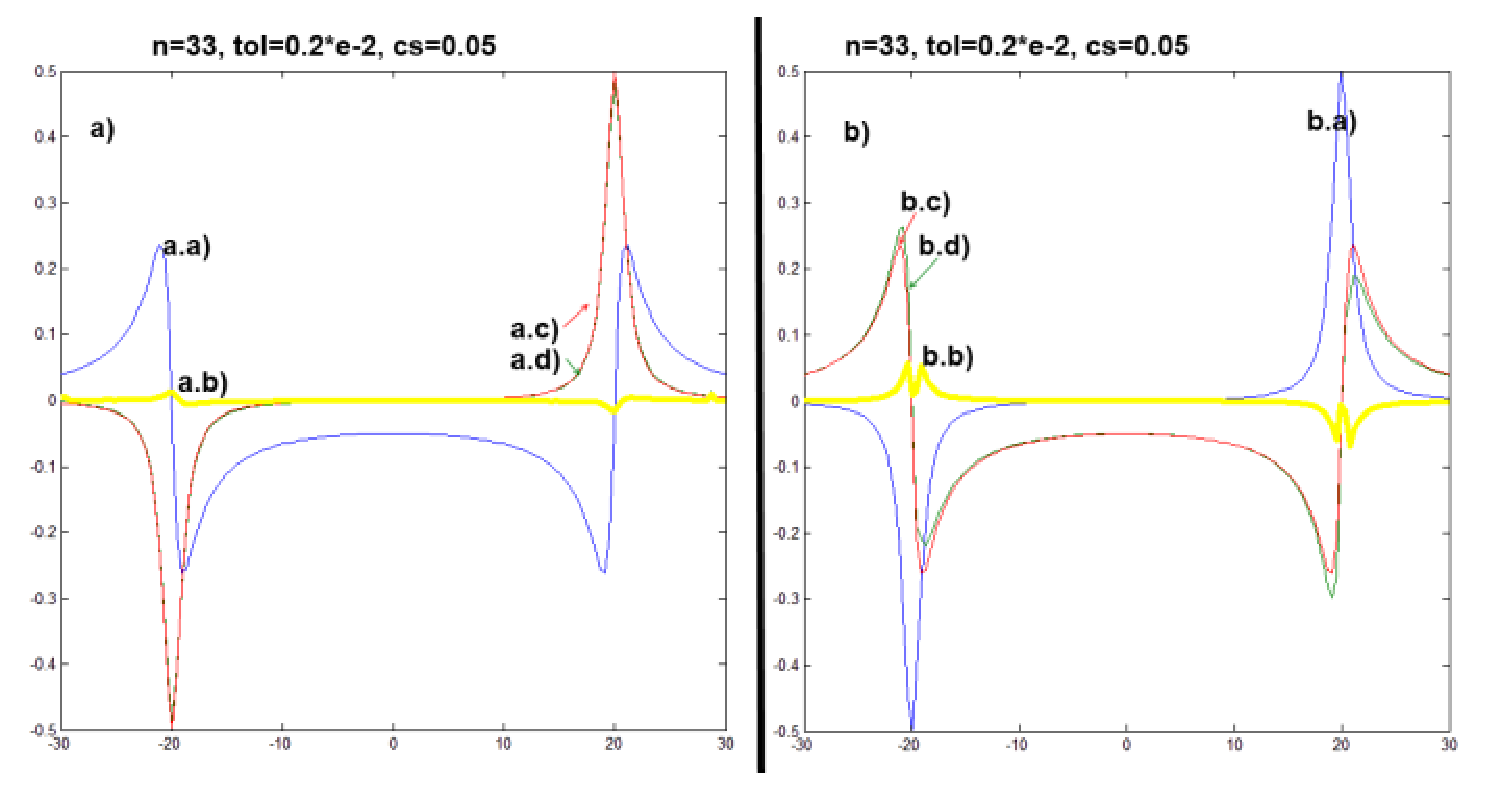
\includegraphics{img/nc_lin4.eps}
{\small [Figure 5.2.4a-b] Calcuations for parameters (
\mapleinline{inert}{2d}{n = 33,tol = .2e-2,cs = .5e-1;}{%
$n=33, \,\mathit{tol}=\mbox{.2e-2}, \,\mathit{cs}=\mbox{.5e-1}$%
}) a.a) The plot of the real part of 
\mapleinline{inert}{2d}{chi(omega);}{%
$\chi (\omega )$%
} a.b) absolute error plot (a.d-plot minus a.c-plot) a.c) imaginary
part of 
\mapleinline{inert}{2d}{chi(omega);}{%
$\chi (\omega )$%
} calculated analytically a.d) imaginary part of 
\mapleinline{inert}{2d}{chi(omega);}{%
$\chi (\omega )$%
} obtained with the Hilbert transform of a.a-plot, b.a) The plot of
the imaginary part of 
\mapleinline{inert}{2d}{chi(omega);}{%
$\chi (\omega )$%
} b.b) absolute error plot (b.d-plot minus b.c-plot) b.c) real part of

\mapleinline{inert}{2d}{chi(omega);}{%
$\chi (\omega )$%
}}{\small  calculated analytically b.d) real part of 
\mapleinline{inert}{2d}{chi(omega);}{%
$\chi (\omega )$%
}} {\small obtained with the Hilbert transform of b.a-plot }





We cannot tell with hundred percent confidence which set of parameters
will fit the best any given function and the user will need to try
many combinations before obtaining the final plot, but what we gave is
the opportunity to set each one parameter manually, which may lead to
better results in the particular cases.





\textit{Example cases for solving the Kramers-Kronig relations in
linear model using modified Newton-Cotes method - with short
conclusions.}




\subsection{NC for simple nonlinear model - results}



We have performed calculations for the same both nonlinear pump-probe
and wave-mixing model as in 4.3. Results for 1-Dimension and
2-Dimensions has been presented below:





\includegraphics[width=170mm]{img/nc_fmix1.eps}
(5.3.1) 
\mapleinline{inert}{2d}{chi[pp](delta) =
G*n[0]*gamma[ba]/(Delta+delta+I*eta)*(1-Omega[1]^2*(Delta-delta+I*eta)
*(delta+2*I*eta)/(Delta-I*eta)/((delta+I*theta)*(Delta+delta+I*eta)*(d
elta-Delta+I*eta)-Omega[1]^2*(delta+I*eta))/2);}{%
${\chi _{\mathit{pp}}}(\delta )=\frac {G\,{n_{0}}\,{\gamma _{
\mathit{ba}}}\, \left(  \! 1 - \frac {{\Omega _{1}}^{2}\,(\Delta 
 - \delta  + I\,\eta )\,(\delta  + 2\,I\,\eta )}{(\Delta  - I\,
\eta )\,((\delta  + I\,\theta )\,(\Delta  + \delta  + I\,\eta )\,
(\delta  - \Delta  + I\,\eta ) - {\Omega _{1}}^{2}\,(\delta  + I
\,\eta ))\,2} \!  \right) }{\Delta  + \delta  + I\,\eta }$%
}     





where:
\mapleinline{inert}{2d}{G = 1;}{%
$G=1$%
}, 
\mapleinline{inert}{2d}{gamma[ba];}{%
${\gamma _{\mathit{ba}}}$%
} = -0.1, 
\mapleinline{inert}{2d}{n[0];}{%
${n_{0}}$%
} = 1, 
\mapleinline{inert}{2d}{Delta = 1.3;}{%
$\Delta =\mbox{1.3}$%
}, 
\mapleinline{inert}{2d}{eta = 1;}{%
$\eta =1$%
}, 
\mapleinline{inert}{2d}{theta = 1.4;}{%
$\theta =\mbox{1.4}$%
}, 
\mapleinline{inert}{2d}{Omega[1] = 4.3;}{%
${\Omega _{1}}=\mbox{4.3}$%
}





(5.3.2) 
\mapleinline{inert}{2d}{chi[mix](delta) =
2/3*N*w[0]*mu[ba]^4*(-delta-Delta-i/T[2])*(delta+2*i/T[2])/(Delta+i/T[
2])/epsilon0/(h^3)/(Delta+delta+i/T[2])/(delta^3-2*i*delta^2/T[2]-delt
a*Delta^2-2*i/T[1]*delta/T[2]-delta/(T[2]^2)+delta^2/T[1]-Delta^2/T[1]
-1/(T[1]*T[2]^2)-Omega[2]*delta+Omega[2]/T[2]*i);}{%
${\chi _{\mathit{mix}}}(\delta )=2\,N\,{w_{0}}\,{\mu _{\mathit{ba
}}}^{4}\,( - \delta  - \Delta  - \frac {i}{{T_{2}}})\,(\delta  + 
\frac {2\,i}{{T_{2}}}) \left/ {\vrule 
height0.90em width0em depth0.90em} \right. \!  \! (3\,(\Delta  + 
\frac {i}{{T_{2}}})\,\varepsilon 0\,h^{3}\,(\Delta  + \delta  + 
\frac {i}{{T_{2}}})\,(\delta ^{3} - \frac {2\,i\,\delta ^{2}}{{T
_{2}}} - \delta \,\Delta ^{2} - \frac {2\,i\,\delta }{{T_{1}}\,{T
_{2}}} - \frac {\delta }{{T_{2}}^{2}} + \frac {\delta ^{2}}{{T_{1
}}} - \frac {\Delta ^{2}}{{T_{1}}} - \frac {1}{{T_{1}}\,{T_{2}}^{
2}} - {\Omega _{2}}\,\delta  + \frac {{\Omega _{2}}\,i}{{T_{2}}})
)$%
}





where:
\mapleinline{inert}{2d}{N = 1,w[0] = 1,mu[ba] = 1,T[1] = 1,T[2] = 2,Omega[2] = 1,epsilon[0] =
1,h = 1,Delta = 1;}{%
$N=1, \,{w_{0}}=1, \,{\mu _{\mathit{ba}}}=1, \,{T_{1}}=1, \,{T_{2
}}=2, \,{\Omega _{2}}=1, \,{\varepsilon _{0}}=1, \,h=1, \,\Delta 
=1$%
}








[Figure 5.3.1a-b] Calcuations for parameters (
\mapleinline{inert}{2d}{n = 8,cs = .3e-2,tol = .1e-1;}{%
$n=8, \,\mathit{cs}=\mbox{.3e-2}, \,\mathit{tol}=\mbox{.1e-1}$%
} a.a) The plot of the real part of 
\mapleinline{inert}{2d}{chi[pp](delta);}{%
${\chi _{\mathit{pp}}}(\delta )$%
} a.b) absolute error plot (a.d-plot minus a.c-plot) a.c) imaginary
part of 
\mapleinline{inert}{2d}{chi[pp](delta);}{%
${\chi _{\mathit{pp}}}(\delta )$%
} calculated analytically a.d) imaginary part of 
\mapleinline{inert}{2d}{chi[pp](delta);}{%
${\chi _{\mathit{pp}}}(\delta )$%
} obtained with the Hilbert transform of a.a-plot, b.a) The plot of
the imaginary part of 
\mapleinline{inert}{2d}{chi[pp](delta);}{%
${\chi _{\mathit{pp}}}(\delta )$%
} b.b) absolute error plot (b.d-plot minus b.c-plot) b.c) real part of

\mapleinline{inert}{2d}{chi(omega);}{%
$\chi (\omega )$%
} calculated analytically b.d) real part of 
\mapleinline{inert}{2d}{chi[pp](delta);}{%
${\chi _{\mathit{pp}}}(\delta )$%
} obtained with the Hilbert transform of b.a-plot 





Example cases for solving the Kramers-Kronig relations in simple
nonlinear model using NC - with short conslusions.




\subsection{NC for simple quantum-perturbative model - results}

\subsubsection*{Linear model - results:}



For the linear susceptibility we have used the model from the chapter
2.5: 





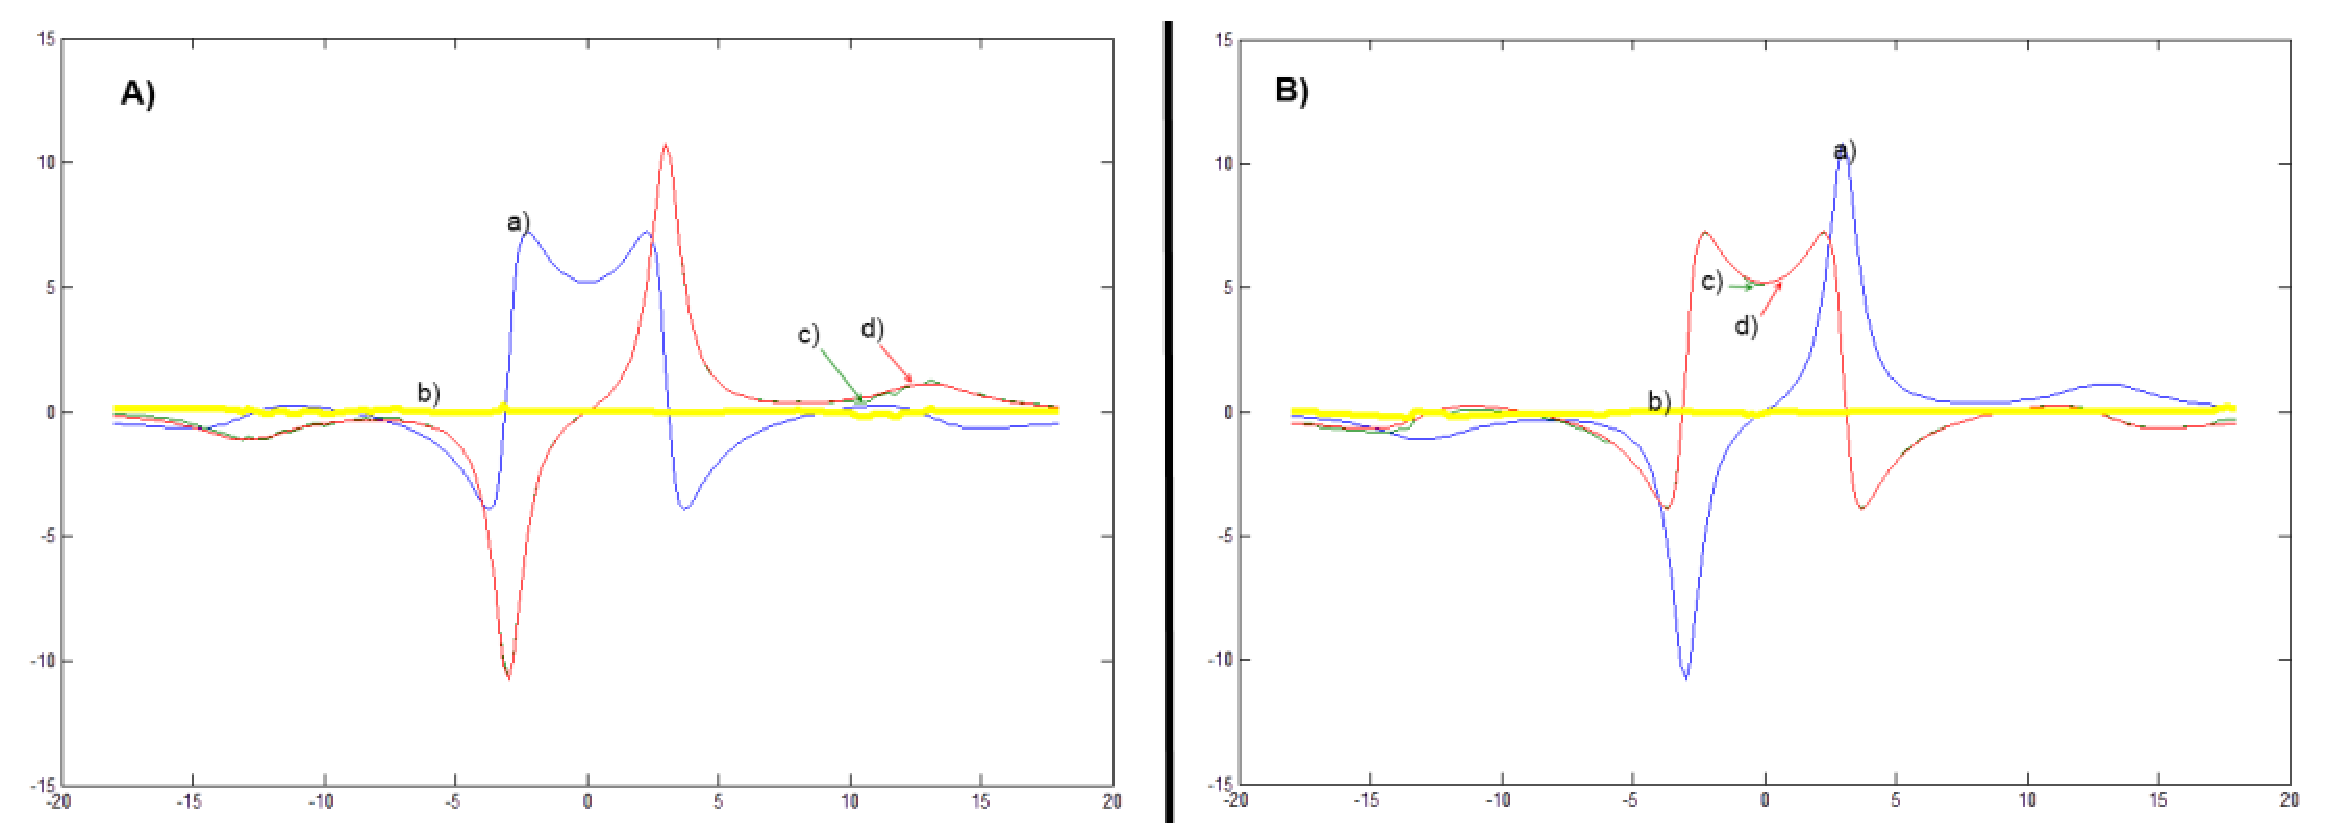
\includegraphics[width=170mm]{img/nc_qp1.eps}
(5.4.1) 
\mapleinline{inert}{2d}{chi[1,qp](omega);}{%
${\chi _{1, \,\mathit{qp}}}(\omega )$%
} = 
\mapleinline{inert}{2d}{sum(mu[1,n]*mu[2,n]/(Omega[n]-omega-i*gamma[n])+mu[2,n]*mu[1,n]/(Omeg
a[n]+omega+i*gamma[n]),n = 1 .. 2)*N/epsilon0/h;}{%
$\frac { \left(  \! \sum _{n=1}^{2}\,(\frac {{\mu _{1, \,n}}\,{
\mu _{2, \,n}}}{{\Omega _{n}} - \omega  - i\,{\gamma _{n}}} + 
\frac {{\mu _{2, \,n}}\,{\mu _{1, \,n}}}{{\Omega _{n}} + \omega 
 + i\,{\gamma _{n}}}) \!  \right) \,N}{\varepsilon 0\,h}$%
}





This time we have used the following parameters:
\mapleinline{inert}{2d}{mu;}{%
$\mu $%
} = 
\mapleinline{inert}{2d}{[[3, -.5], [1.2, 2.4]];}{%
$[[3, \, - \mbox{.5}], \,[\mbox{1.2}, \,\mbox{2.4}]]$%
}, 
\mapleinline{inert}{2d}{Omega = [-3, 13];}{%
$\Omega =[ - 3, \,13]$%
}, 
\mapleinline{inert}{2d}{gamma = [.7, 2.3];}{%
$\gamma =[\mbox{.7}, \,\mbox{2.3}]$%
}, 
\mapleinline{inert}{2d}{N = 8;}{%
$N=8$%
}, 
\mapleinline{inert}{2d}{epsilon[0] = 1.4,h = -2.7;}{%
${\varepsilon _{0}}=\mbox{1.4}, \,h= - \mbox{2.7}$%
}





Evaluation time of two plots given in the Figures (5.4.1a-b) was 615
seconds.






{\small [Figures 5.4.1a-b] Results plotted together 
[5.4.1.a] A: a) The plot of the imag part of 
\mapleinline{inert}{2d}{chi[1,qp](delta);}{%
${\chi _{1, \,\mathit{qp}}}(\delta )$%
}} {\small b) absolute error plot (d-plot minus c-plot) d) real part
of 
\mapleinline{inert}{2d}{chi[1,qp](delta);}{%
${\chi _{1, \,\mathit{qp}}}(\delta )$%
}} {\small obtained with the Hilbert transform of a-plot d) real part
of 
\mapleinline{inert}{2d}{chi[pp](delta);}{%
${\chi _{\mathit{pp}}}(\delta )$%
}}{\small  calculated analytically 
[5.4.1.b] B: b) The plot of the real part of 
\mapleinline{inert}{2d}{chi[1,qp](delta);}{%
${\chi _{1, \,\mathit{qp}}}(\delta )$%
}} {\small b) absolute error plot (d-plot minus c-plot) c) imaginary
part of 
\mapleinline{inert}{2d}{chi[1,qp](delta);}{%
${\chi _{1, \,\mathit{qp}}}(\delta )$%
}} {\small obtained with the Hilbert transform of a-plot d) imaginary
part of 
\mapleinline{inert}{2d}{chi[pp](delta);}{%
${\chi _{\mathit{pp}}}(\delta )$%
}}{\small  calculated analytically  }




\subsubsection*{Second-order model - results:}



For the linear susceptibility we have used the model from the chapter
2.5: 





(5.4.2) 
\mapleinline{inert}{2d}{chi[2, qp](omega[1],omega[2]) =
N/2/epsilon[0]/(h^2)*sum(sum(sum(mu[l,n]*mu[nm]*mu[ml]/(Omega[nl]-omeg
a1-omega2-i*gamma[nl])/(Omega[ml]-omega1-i*gamma[ml])+mu[l,n]*mu[nm]*m
u[ml]/(Omega[nl]-omega1-omega1-i*gamma[nl])/(Omega[ml]-omega2-i*gamma[
ml])+mu[l,n]*mu[nm]*mu[ml]/(Omega[mn]-omega1-omega2-i*gamma[mn])/(Omeg
a[nl]+omega2+i*gamma[nl])+mu[l,n]*mu[nm]*mu[ml]/(Omega[mn]-omega1-omeg
a2-i*gamma[mn])/(Omega[nl]+omega2+i*gamma[nl])+mu[l,n]*mu[nm]*mu[ml]/(
Omega[nm]+omega1+omega2+i*gamma[nm])/(Omega[ml]-omega1-i*gamma[ml])+mu
[l,n]*mu[nm]*mu[ml]/(Omega[nm]+omega1+omega2+i*gamma[nm])/(Omega[ml]-o
mega1-i*gamma[ml])+mu[l,n]*mu[nm]*mu[ml]/(Omega[ml]+omega1+omega2+i*ga
mma[ml])/(Omega[nl]+omega1+i*gamma[nl])+mu[l,n]*mu[nm]*mu[ml]/(Omega[m
l]+omega1+omega2+i*gamma[ml])/(Omega[nl]+omega2+i*gamma[nl]),l = 1 ..
2),m = 1 .. 2),n = 1 .. 2);}{%
${\chi _{2, \,\mathit{qp}}}({\omega _{1}}, \,{\omega _{2}})=N\,
 \left(  \! \sum _{n=1}^{2}\, \left(  \! \sum _{m=1}^{2}\,
 \left(  \! \sum _{l=1}^{2}\,(\frac {{\mu _{l, \,n}}\,{\mu _{
\mathit{nm}}}\,{\mu _{\mathit{ml}}}}{({\Omega _{\mathit{nl}}} - 
\omega 1 - \omega 2 - i\,{\gamma _{\mathit{nl}}})\,({\Omega _{
\mathit{ml}}} - \omega 1 - i\,{\gamma _{\mathit{ml}}})} + \frac {
{\mu _{l, \,n}}\,{\mu _{\mathit{nm}}}\,{\mu _{\mathit{ml}}}}{({
\Omega _{\mathit{nl}}} - \omega 1 - \omega 1 - i\,{\gamma _{
\mathit{nl}}})\,({\Omega _{\mathit{ml}}} - \omega 2 - i\,{\gamma 
_{\mathit{ml}}})} + \frac {{\mu _{l, \,n}}\,{\mu _{\mathit{nm}}}
\,{\mu _{\mathit{ml}}}}{({\Omega _{\mathit{mn}}} - \omega 1 - 
\omega 2 - i\,{\gamma _{\mathit{mn}}})\,({\Omega _{\mathit{nl}}}
 + \omega 2 + i\,{\gamma _{\mathit{nl}}})} + \frac {{\mu _{l, \,n
}}\,{\mu _{\mathit{nm}}}\,{\mu _{\mathit{ml}}}}{({\Omega _{
\mathit{mn}}} - \omega 1 - \omega 2 - i\,{\gamma _{\mathit{mn}}})
\,({\Omega _{\mathit{nl}}} + \omega 2 + i\,{\gamma _{\mathit{nl}}
})} + \frac {{\mu _{l, \,n}}\,{\mu _{\mathit{nm}}}\,{\mu _{
\mathit{ml}}}}{({\Omega _{\mathit{nm}}} + \omega 1 + \omega 2 + i
\,{\gamma _{\mathit{nm}}})\,({\Omega _{\mathit{ml}}} - \omega 1
 - i\,{\gamma _{\mathit{ml}}})} + \frac {{\mu _{l, \,n}}\,{\mu _{
\mathit{nm}}}\,{\mu _{\mathit{ml}}}}{({\Omega _{\mathit{nm}}} + 
\omega 1 + \omega 2 + i\,{\gamma _{\mathit{nm}}})\,({\Omega _{
\mathit{ml}}} - \omega 1 - i\,{\gamma _{\mathit{ml}}})} + \frac {
{\mu _{l, \,n}}\,{\mu _{\mathit{nm}}}\,{\mu _{\mathit{ml}}}}{({
\Omega _{\mathit{ml}}} + \omega 1 + \omega 2 + i\,{\gamma _{
\mathit{ml}}})\,({\Omega _{\mathit{nl}}} + \omega 1 + i\,{\gamma 
_{\mathit{nl}}})} + \frac {{\mu _{l, \,n}}\,{\mu _{\mathit{nm}}}
\,{\mu _{\mathit{ml}}}}{({\Omega _{\mathit{ml}}} + \omega 1 + 
\omega 2 + i\,{\gamma _{\mathit{ml}}})\,({\Omega _{\mathit{nl}}}
 + \omega 2 + i\,{\gamma _{\mathit{nl}}})}) \!  \right)  \! 
 \right)  \!  \right)  \left/ {\vrule 
height0.47em width0em depth0.47em} \right. \!  \! (2\,{
\varepsilon _{0}}\,h^{2})$%
}





where:
\mapleinline{inert}{2d}{mu;}{%
$\mu $%
} = 
\mapleinline{inert}{2d}{[[1, 3], [-1, -2]];}{%
$[[1, \,3], \,[ - 1, \, - 2]]$%
}, 
\mapleinline{inert}{2d}{Omega = [[3, 16], [4, 12]];}{%
$\Omega =[[3, \,16], \,[4, \,12]]$%
}, 
\mapleinline{inert}{2d}{gamma = [[1, 2], [-1, 3]];}{%
$\gamma =[[1, \,2], \,[ - 1, \,3]]$%
}, 
\mapleinline{inert}{2d}{N = 5;}{%
$N=5$%
}, 
\mapleinline{inert}{2d}{epsilon[0] = 1,h = -1;}{%
${\varepsilon _{0}}=1, \,h= - 1$%
}




\emptyline



Example cases for solving the Kramers-Kronig relations in simple
\textit{quantum-}perturbative model using NC - with short conslusions.




\subsection{NC for other models - results}



Text and graphs here... 





Example cases for solving the Kramers-Kronig relations for other
models using NC - with short conslusions.




\section{Hilbert Clenshaw-Curtis iterations (solving)}

\subsection{Overview of the Hilbert Clenshaw-Curtis iterations}



The adaptive and iterative algorithm for obtaining the Hilbert
transform of a given regime of abscissas is presented. 




\subsubsection*{Clenshaw Curtis quadrature: }



The heart of the calculation is based on the typical Clenshaw-Curtis
quadrature of function that has been expanded into a form of Chebyshev
polynomials. We define the quadrature problem as follows - for a given
function f(x) find a value of the integral:





(6.1.1) CCI = 
\mapleinline{inert}{2d}{int(f(x),x = -1 .. 1);}{%
$\int _{ - 1}^{1}\mathrm{f}(x)\,dx$%
}





The first step in solving this quadrature, after the idea of C.W.
Clenshaw and A.R. Curtis [25] is to do the following change of
variables:





(6.1.2a) 
\mapleinline{inert}{2d}{x = cos(theta);}{%
$x=\mathrm{cos}(\theta )$%
}
(6.1.2b) CCI = 
\mapleinline{inert}{2d}{int(f(cos(theta))*sin(theta),theta = 0 .. Pi);}{%
$\int _{0}^{\pi }\mathrm{f}(\mathrm{cos}(\theta ))\,\mathrm{sin}(
\theta )\,d\theta $%
}





By using the Discrete Cosine Transform of I-type, we can estimate the
integral (6.1.2b) with following series:





(6.1.3a) 
\mapleinline{inert}{2d}{int(f(cos(theta))*sin(theta),theta = 0 .. Pi);}{%
$\int _{0}^{\pi }\mathrm{f}(\mathrm{cos}(\theta ))\,\mathrm{sin}(
\theta )\,d\theta $%
} \symbol{126}= 
\mapleinline{inert}{2d}{a[0]+sum(2*a[2*k]/(1-(2*k)^2),k = 1 .. N/2-1)+a[N]/(1-N^2);}{%
${a_{0}} +  \left(  \! \sum _{k=1}^{\frac {N}{2} - 1}\,\frac {2\,
{a_{2\,k}}}{1 - (2\,k)^{2}} \!  \right)  + \frac {{a_{N}}}{1 - N
^{2}}$%
}
(6.1.3b) 
\mapleinline{inert}{2d}{a[k] = 2/pi*int(f*cos(theta)*cos(k*theta),theta = 0 .. pi);}{%
${a_{k}}=\frac {2\,\int _{0}^{\pi }f\,\mathrm{cos}(\theta )\,
\mathrm{cos}(k\,\theta )\,d\theta }{\pi }$%
}





Now we perform the simple approximation of (6.1.3b) with:





(6.1.4) 
\mapleinline{inert}{2d}{a[k];}{%
${a_{k}}$%
} \symbol{126}= 
\mapleinline{inert}{2d}{2/N*(f(1)/2+f(-1)/2*(-1)^k+sum(f(cos(n*pi/N))*cos(n*pi/N*k),k = 1 ..
N-1));}{%
$\frac {2\, \left(  \! \frac {\mathrm{f}(1)}{2} + \frac {\mathrm{
f}( - 1)\,( - 1)^{k}}{2} +  \left(  \! \sum _{k=1}^{N - 1}\,
\mathrm{f}(\mathrm{cos}(\frac {n\,\pi }{N}))\,\mathrm{cos}(
\frac {n\,\pi \,k}{N}) \!  \right)  \!  \right) }{N}$%
} 





And while in the (6.1.3a) equation we need only 
\mapleinline{inert}{2d}{a[2*k];}{%
${a_{2\,k}}$%
}, the (6.1.4) equation can be simplified:





(6.1.5) 
\mapleinline{inert}{2d}{a[2*k];}{%
${a_{2\,k}}$%
} \symbol{126}= 
\mapleinline{inert}{2d}{2/N*((f(1)-f(-1))/2+f(0)^(-k)+sum(f(cos(pi*n/N))+f(-cos(pi*n/N))*cos(
n*k*pi/(N/2)),k = 1 .. N/2-1));}{%
$\frac {2\, \left(  \! \frac {\mathrm{f}(1) - \mathrm{f}( - 1)}{2
} + \mathrm{f}(0)^{( - k)} +  \left(  \! \sum _{k=1}^{\frac {N}{2
} - 1}\, \left(  \! \mathrm{f}(\mathrm{cos}(\frac {\pi \,n}{N}))
 + \mathrm{f}( - \mathrm{cos}(\frac {\pi \,n}{N}))\,\mathrm{cos}
 \left(  \! \frac {n\,k\,\pi }{\frac {N}{2}} \!  \right)  \! 
 \right)  \!  \right)  \!  \right) }{N}$%
}





We can now simplify the (6.1.5) equation using the matrix notation:





(6.1.6a) 
\mapleinline{inert}{2d}{y[n] = f(cos(pi*n/N)+f(-cos(n*pi/N)));}{%
${y_{n}}=\mathrm{f}(\mathrm{cos}(\frac {\pi \,n}{N}) + \mathrm{f}
( - \mathrm{cos}(\frac {n\,\pi }{N})))$%
}
(6.1.6b) 
\mapleinline{inert}{2d}{D[k,n] = 2/N*cos(n*k*pi/(N/2))*C[k];}{%
${\mathrm{D}_{k, \,n}}=\frac {2\,\mathrm{cos} \left(  \! \frac {n
\,k\,\pi }{\frac {N}{2}} \!  \right) \,{C_{k}}}{N}$%
}





where:
\mapleinline{inert}{2d}{C[k] = 1/2;}{%
${C_{k}}=\frac {1}{2}$%
} for k = 0, N/2 and otherwise 
\mapleinline{inert}{2d}{C[k] = 1;}{%
${C_{k}}=1$%
}





We can observe, that both (6.1.5) and (6.1.6a-b) describes the DCT-I
transform. Now we use the statement, that DCT-I is equivalent to a DFT
of 2N - 2 real numbers with even symmetry. So we state:





(6.1.7a) 
\mapleinline{inert}{2d}{Y[m] = y[2*m] and Y[N-1-m] = x[2*m+1];}{%
${Y_{m}}={y_{2\,m}}\ \textbf{and}\ {Y_{N - 1 - m}}={x_{2\,m + 1}}
$%
} for (m=0,1,...,N/2-1)
(6.1.7b) FY = DFT(Y)
(6.1.7c) [a] = DCT-I(y) = 
\mapleinline{inert}{2d}{Re(exp(-j*n*pi/(2*N))*FY);}{%
$\Re (e^{( - \frac {j\,n\,\pi }{2\,N})}\,\mathit{FY})$%
}





Now as we got the vector of a coefficients (6.1.7c) we can perform the
final calculation by multiplying with vector d:





(6.1.8) 
\mapleinline{inert}{2d}{d[0];}{%
${d_{0}}$%
} = 1, 
\mapleinline{inert}{2d}{d[2*k] = 2/(1-(2*k)^2);}{%
${d_{2\,k}}=\frac {2}{1 - (2\,k)^{2}}$%
}, 
\mapleinline{inert}{2d}{d[N] = 1/(1-N^2);}{%
${d_{N}}=\frac {1}{1 - N^{2}}$%
}





And we get the final conslusion:





(6.1.9) 
\mapleinline{inert}{2d}{int(f(x),x = -1 .. 1) = d^T*[a];}{%
$\int _{ - 1}^{1}\mathrm{f}(x)\,dx=d^{T}\,[a]$%
}




\subsubsection*{Hilbert transform using the Clenshaw-Curtis
quadrature:}



While the Clenshaw-Curtis quadrature is defined for finite range
[-1,1], the Hilbert transform uses the definite and improper integral
over the range [-infinity, infinity]. What must now be done is to
change the range of integrations without changing the value of the
Hilbert transform:





(6.1.10a) x = 
\mapleinline{inert}{2d}{t/(1-t^2);}{%
$\frac {t}{1 - t^{2}}$%
}
(6.1.10b) \textbf{Hil(f)(s)} =  
\mapleinline{inert}{2d}{1/Pi*int(f(x)/(x-s),x = -infinity .. infinity);}{%
$\frac {1\,\int _{ - \infty }^{\infty }\frac {\mathrm{f}(x)}{x - 
s}\,dx}{\pi }$%
} = 
\mapleinline{inert}{2d}{1/Pi*int(f(t/(1-t^2))*(1+t^2)/((t^2-1)*(t+s*t^2-s)),t = -1 .. 1);}{%
$\frac {1\,\int _{ - 1}^{1}\frac {\mathrm{f}(\frac {t}{1 - t^{2}}
)\,(1 + t^{2})}{(t^{2} - 1)\,(t + s\,t^{2} - s)}\,dt}{\pi }$%
} 





Our simple algorithm uses the implementation of Clenshaw-Curtis
quadrature with the inner function:





(6.1.11) g(t,s) = 
\mapleinline{inert}{2d}{f(t/(1-t^2))*(1+t^2)/((t^2-1)*(t+s*t^2-s));}{%
$\frac {\mathrm{f}(\frac {t}{1 - t^{2}})\,(1 + t^{2})}{(t^{2} - 1
)\,(t + s\,t^{2} - s)}$%
}





In our implementation is adaptive - we compare two results for number
of points N and 2*N - if the result is satisfactory, the loop ends, if
not - we continue with doubling the number of points in the
Clenshaw-Curtis quadrature implementation - so the step and tolerance
must be selecter wisely.




\subsubsection*{Our implementation of the Hilbert Clenshaw-Curtis
iterations:}



So fare we have presented the overview of procedures responsible for
evaluation of the Clenshaw-Curtis quadrature and the Hilbert transform
using the Clenshaw-Curtis quadrature in one point. But in the typical
situation we have the whole vector of function values for a given
range of abscissas - so what is left - we perform the single-point
Hilbert transform based on the Clenshaw-Curtis quadrature for each
given point. But to omit problems with singularities, we will add some
post- and precalculations - using the cubic interpolation. The whole
procedure is now:





\textbf{INPUT: 
}X, Y - given N-length abscissas and related ordinates
\textbf{PRE-CALCULATIONS:
}From N points of Y we calculate the cubic interpolation having N-1
inner points:





(6.1.12a) 
\mapleinline{inert}{2d}{Yp[1] = (3*Y[1]+6*Y[2]-Y[3])/8;}{%
${\mathit{Yp}_{1}}=\frac {3\,{Y_{1}} + 6\,{Y_{2}} - {Y_{3}}}{8}$%
}



(6.1.12b) 
\mapleinline{inert}{2d}{Yp[k] = (-Y[k-1]+9*Y[k]+9*Y[k+1]-Y[k+2])/16;}{%
${\mathit{Yp}_{k}}=\frac { - {Y_{k - 1}} + 9\,{Y_{k}} + 9\,{Y_{k
 + 1}} - {Y_{k + 2}}}{16}$%
}
(6.1.12c) 
\mapleinline{inert}{2d}{Yp[N] = (-Y[N-2]+6*Y[N-1]+3*Y[N])/8;}{%
${\mathit{Yp}_{N}}=\frac { - {Y_{N - 2}} + 6\,{Y_{N - 1}} + 3\,{Y
_{N}}}{8}$%
}





\textbf{MAIN CALCULATIONS:
}With desired tolerance we calculate the N-1 values for each on of
inner points:





(6.1.13) 
\mapleinline{inert}{2d}{Hh[k];}{%
${\mathit{Hh}_{k}}$%
} \symbol{126}= \textbf{Hil(f)(
\mapleinline{inert}{2d}{Yp[k];}{%
${\mathit{Yp}_{k}}$%
})}





\textbf{POST-CALCULATIONS:
}From N-1 points of Hh we calculate N points using the reverse cubic
interpolation





(6.1.14a) 
\mapleinline{inert}{2d}{H[1] = (15*Hh[1]-10*Hh[2]+3*Hh[3])/8;}{%
${H_{1}}=\frac {15\,{\mathit{Hh}_{1}} - 10\,{\mathit{Hh}_{2}} + 3
\,{\mathit{Hh}_{3}}}{8}$%
}
(6.1.14b) 
\mapleinline{inert}{2d}{H[2] = (3*Hh[1]+6*Hh[2]-Hh[3])/8;}{%
${H_{2}}=\frac {3\,{\mathit{Hh}_{1}} + 6\,{\mathit{Hh}_{2}} - {
\mathit{Hh}_{3}}}{8}$%
}
(6.1.14c) 
\mapleinline{inert}{2d}{H[k] = (-Hh[k-1]+9*Hh[k]+9*Hh[k+1]-Hh[k+2])/16;}{%
${H_{k}}=\frac { - {\mathit{Hh}_{k - 1}} + 9\,{\mathit{Hh}_{k}}
 + 9\,{\mathit{Hh}_{k + 1}} - {\mathit{Hh}_{k + 2}}}{16}$%
}
(6.1.14d) 
\mapleinline{inert}{2d}{H[N-1] = (-Hh[N-3]+6*Hh[2]-Hh[3])/8;}{%
${H_{N - 1}}=\frac { - {\mathit{Hh}_{N - 3}} + 6\,{\mathit{Hh}_{2
}} - {\mathit{Hh}_{3}}}{8}$%
}
(6.1.14e) 
\mapleinline{inert}{2d}{H[N] = (3*Hh[N-3]-10*Hh[N-2]+15*Hh[N-1])/8;}{%
${H_{N}}=\frac {3\,{\mathit{Hh}_{N - 3}} - 10\,{\mathit{Hh}_{N - 
2}} + 15\,{\mathit{Hh}_{N - 1}}}{8}$%
}





\textbf{OUTPUT:}



H - N-length hilbert transform for given function values at X
abscissas





The algorithm source has been presented in the Appendix A.3





O\textit{verview of the }Clenshaw-Curtis iterations\textit{ method.}




\subsection{HCCI for simple linear model}



Text and graphs here.... 





\textit{Example cases for solving the Kramers-Kronig relations in
linear model using }CCI\textit{ - with short conclusions.}




\subsection{HCCI for simple nonlinear model}



Text and graphs here.... 





\textit{Example cases for solving the Kramers-Kronig relations in
simple nonlinear model using CCI - with short conslusions.}




\subsection{HCCI for simple quantum-perturbative model}



Text and graphs here.... 





\textit{Example cases for solving the Kramers-Kronig relations in
simple quantum-perturbative model using CCI - with short conslusions.}




\subsection{HCCI for other models}



Text and graphs here.... 





\textit{Example cases for solving the Kramers-Kronig relations for
other models using CCI - with short conslusions.}




\section{Fast Hartley transform approach (solving)}

\subsection{Overview of the FTHA}



The Fast Hartley Transform approach for the Hilbert transform is based
on two efficient O (n log n) discrete Hartley transforms and was well
described by Soo-Chang Pei in [26]. This approach is faster than
another discrete Hilbert transform based on two Fourier transorms,
because the whole computation are carried using only real numbers,
which is faster than Fourier computation carried using time consuming
complex numbers.




\subsubsection*{Discrete Hartley Transform}



For a given N-lenght vector X both the discrete Hartley transform and
inverse discrete Hartley transform are defined as follows:





(7.1.1a) 
\mapleinline{inert}{2d}{DHT(X[k]) = sum(X[n]*(cos(2*pi*k*n/N)+sin(2*Pi*k*n/N)),n = 0 ..
N-1);}{%
$\mathrm{DHT}({X_{k}})=\sum _{n=0}^{N - 1}\,{X_{n}}\,(\mathrm{cos
}(\frac {2\,\pi \,k\,n}{N}) + \mathrm{sin}(\frac {2\,\pi \,k\,n}{
N}))$%
}
(7.1.1b) 
\mapleinline{inert}{2d}{IDHT(H[k]) = sum(H[n]*(cos(2*pi*k*n/N)+sin(2*Pi*k*n/N)),k = 0 ..
N-1)/N;}{%
$\mathrm{IDHT}({H_{k}})=\frac {\sum _{k=0}^{N - 1}\,{H_{n}}\,(
\mathrm{cos}(\frac {2\,\pi \,k\,n}{N}) + \mathrm{sin}(\frac {2\,
\pi \,k\,n}{N}))}{N}$%
}




\subsubsection*{Hartley transform convolution theorem}



Now we will introduce the Hartley transform convolution theorem. We
define the N-lenght vector x as convolution of two N-length vectors 
\mapleinline{inert}{2d}{x[1];}{%
${x_{1}}$%
}, 
\mapleinline{inert}{2d}{x[2];}{%
${x_{2}}$%
} as follows:





(7.1.2) 
\mapleinline{inert}{2d}{x[n] = x[1,n];}{%
${x_{n}}={x_{1, \,n}}$%
} * 
\mapleinline{inert}{2d}{x[2,n];}{%
${x_{2, \,n}}$%
} = 
\mapleinline{inert}{2d}{sum(x[1,k]*x[2,n-k],k = 0 .. N-1);}{%
$\sum _{k=0}^{N - 1}\,{x_{1, \,k}}\,{x_{2, \,n - k}}$%
}





For a given convolution, the following theorem is stated:





(7.1.3) 
\mapleinline{inert}{2d}{DHT(x[n]) =
DHT(x[1,k])*even(DHT(x[2,k]))+DHT(x[1,-k])*odd(DHT(h[2,k]));}{%
$\mathrm{DHT}({x_{n}})=\mathrm{DHT}({x_{1, \,k}})\,\mathrm{even}(
\mathrm{DHT}({x_{2, \,k}})) + \mathrm{DHT}({x_{1, \, - k}})\,
\mathrm{odd}(\mathrm{DHT}({h_{2, \,k}}))$%
}





where:
\mapleinline{inert}{2d}{DHT(x[2,k]) = even(DHT(x[2,k]))+odd(DHT(x[2,k]));}{%
$\mathrm{DHT}({x_{2, \,k}})=\mathrm{even}(\mathrm{DHT}({x_{2, \,k
}})) + \mathrm{odd}(\mathrm{DHT}({x_{2, \,k}}))$%
}





The proof of the Hartley transform convolution theorem can be found in
[26]. 




\subsubsection*{Relation between discrete Fourier and discrete Hilbert
transform}



Now we will derive the discrete Fourier transform of the Hilbert
transform for a given N-lenght vector x:





(7.1.4a) 
\mapleinline{inert}{2d}{DFT(DISCRETE_HILBERT(x[k])) = DFT(h(k))*DFT(x[k]);}{%
$\mathrm{DFT}(\mathrm{DISCRETE\_HILBERT}({x_{k}}))=\mathrm{DFT}(
\mathrm{h}(k))\,\mathrm{DFT}({x_{k}})$%
} = 
\mapleinline{inert}{2d}{(-i)*sgn(k)*DFT(x[k]);}{%
$( - i)\,\mathrm{sgn}(k)\,\mathrm{DFT}({x_{k}})$%
}





where: 
(7.1.5a) 
\mapleinline{inert}{2d}{H(k) = DFT(h[k]);}{%
$\mathrm{H}(k)=\mathrm{DFT}({h_{k}})$%
}
(7.1.5b) 
\mapleinline{inert}{2d}{h[k] = 1/pi/k;}{%
${h_{k}}=\frac {1}{\pi \,k}$%
} discrete Hilbert kernel





and also:





(7.1.6a) H(k) = i  for 
\mapleinline{inert}{2d}{k = 1,2 .. N/2-1;}{%
$k=1, \,2 .. \frac {N}{2} - 1$%
}
(7.1.6b) H(k) = 0 for 
\mapleinline{inert}{2d}{k = 0,N/2;}{%
$k=0, \,\frac {N}{2}$%
}
(7.1.6c) H(k) = -i for 
\mapleinline{inert}{2d}{k = N/2+1,N/2+2 .. N-1;}{%
$k=\frac {N}{2} + 1, \,\frac {N}{2} + 2 .. N - 1$%
}




\subsubsection*{Application of the discrete Hartley transform to
calculate the discrete Hilbert transform:}



Using the Hartley transform convolution theorem (7.1.3) for a given
N-lenght vector x we obtain:





(7.1.7) 
\mapleinline{inert}{2d}{DHT(DISCRETE_HILBERT(x[k])) =
DHT(x[k])*even(DHT(h[k]))+DHT(x[-k])*odd(DHT(h[k]));}{%
$\mathrm{DHT}(\mathrm{DISCRETE\_HILBERT}({x_{k}}))=\mathrm{DHT}({
x_{k}})\,\mathrm{even}(\mathrm{DHT}({h_{k}})) + \mathrm{DHT}({x_{
 - k}})\,\mathrm{odd}(\mathrm{DHT}({h_{k}}))$%
}
where:
\mapleinline{inert}{2d}{x[-k] = x[`mod`(N-k,N)];}{%
${x_{ - k}}={x_{(N - k)\,\mathrm{mod}\,N}}$%
} (time reversal)





Now we should notice, that the discrete Hilbert transform kernel
defined in (7.1.5b) is an odd function, so its even part equals zero.
So (7.1.7) simplifies now into a product of two separate Hartley
transforms:





(7.1.8) 
\mapleinline{inert}{2d}{DHT(DISCRETE_HILBERT(x[k])) = DHT(x[-k])*odd(DHT(h[k]));}{%
$\mathrm{DHT}(\mathrm{DISCRETE\_HILBERT}({x_{k}}))=\mathrm{DHT}({
x_{ - k}})\,\mathrm{odd}(\mathrm{DHT}({h_{k}}))$%
} = 
\mapleinline{inert}{2d}{DHT(x[-k])*DHT(h[k]);}{%
$\mathrm{DHT}({x_{ - k}})\,\mathrm{DHT}({h_{k}})$%
}





By [26] the second transform is defined:





(7.1.9a) 
\mapleinline{inert}{2d}{DHT(h[k]) = 1;}{%
$\mathrm{DHT}({h_{k}})=1$%
} for 
\mapleinline{inert}{2d}{k = 1,2 .. N/2-1;}{%
$k=1, \,2 .. \frac {N}{2} - 1$%
}
(7.1.9a) 
\mapleinline{inert}{2d}{DHT(h[k]) = 0;}{%
$\mathrm{DHT}({h_{k}})=0$%
} for 
\mapleinline{inert}{2d}{k = 0,N/2;}{%
$k=0, \,\frac {N}{2}$%
}
(7.1.9a) 
\mapleinline{inert}{2d}{DHT(h[k]) = -1;}{%
$\mathrm{DHT}({h_{k}})= - 1$%
} for 
\mapleinline{inert}{2d}{k = N/2+1,N/2+2 .. N-1;}{%
$k=\frac {N}{2} + 1, \,\frac {N}{2} + 2 .. N - 1$%
}





If order to calculate the Hilbert of a given N-lenght vector x the
last thing to do is apply the inverse discrete Hartley transform on
the very right side of (7.1.8) equation. 




\subsubsection*{Fast Hartley Transform algorithm}



Ronald F. Ullmann has showed the fast algorithm for the discrete
Hartley transform in [27]. The important assumption is that - as for
the fast Fourier transform algorithm, the fast Hartley transform
algorithm is defined for a K-length vector x, where K is the
power-of-two:





(7.1.10) \$ 
\mapleinline{inert}{2d}{`in`(p,N);}{%
$p\,\ \textbf{in}\ \,N$%
} :  
\mapleinline{inert}{2d}{K = 2^p;}{%
$K=2^{p}$%
}





The (7.1.10) condition for the algorithm and the further possibilities
to modify it are discussed further. We will start with the very same
thing as in the fast Fourier algorithm - we split the x vector into
two smaller vectors:





(7.1.11a)  
\mapleinline{inert}{2d}{x[1,m/2] = x[m];}{%
${x_{1, \,\frac {m}{2}}}={x_{m}}$%
}     for 
\mapleinline{inert}{2d}{m = 0,2 .. N-1;}{%
$m=0, \,2 .. N - 1$%
}
(7.1.11b)  
\mapleinline{inert}{2d}{x[2,(m-1)/2] = x[m];}{%
${x_{2, \,\frac {m - 1}{2}}}={x_{m}}$%
} for 
\mapleinline{inert}{2d}{m = 1,3 .. N-2;}{%
$m=1, \,3 .. N - 2$%
}





Taking into account the initial definition of the discrete Hartley
transform (7.1.1a), we obtain:





(7.1.12) 
\mapleinline{inert}{2d}{DHT(x[k]) = sum(x(2*n)*(cos(2*pi*k*2*n/N)+sin(2*pi*k*2*n/N)),n = 0 ..
N/2-1)+sum(x(2*n+1)*(cos(2*pi*k*(2*n+1)/N)+sin(2*pi*k*(2*n+1)/N)),n =
0 .. N/2-1);}{%
$\mathrm{DHT}({x_{k}})= \left(  \! \sum _{n=0}^{\frac {N}{2} - 1}
\,\mathrm{x}(2\,n)\,(\mathrm{cos}(\frac {2\,\pi \,k\,2\,n}{N}) + 
\mathrm{sin}(\frac {2\,\pi \,k\,2\,n}{N})) \!  \right)  + 
 \left(  \! \sum _{n=0}^{\frac {N}{2} - 1}\,\mathrm{x}(2\,n + 1)
\,(\mathrm{cos}(\frac {2\,\pi \,k\,(2\,n + 1)}{N}) + \mathrm{sin}
(\frac {2\,\pi \,k\,(2\,n + 1)}{N})) \!  \right) $%
}





In [27] the following ''shift rule'' for the discrete Hartley transform
is stated :





(7.1.13) 
\mapleinline{inert}{2d}{DHT(x[k+c]) = DHT(x[k])*cos(c)+DHT(x[-k])*sin(c);}{%
$\mathrm{DHT}({x_{k + c}})=\mathrm{DHT}({x_{k}})\,\mathrm{cos}(c)
 + \mathrm{DHT}({x_{ - k}})\,\mathrm{sin}(c)$%
}





If we apply the Hartley shift rule (7.1.13) to the splitted equation
in (7.1.12) we obtain:





(7.1.14) 
\mapleinline{inert}{2d}{DHT(x[k]) =
DHT(x[1,k])+cos(2*pi*k/N)*DHT(x[2,k])+sin(2*pi*k/N)*DHT(x[2,-k]);}{%
$\mathrm{DHT}({x_{k}})=\mathrm{DHT}({x_{1, \,k}}) + \mathrm{cos}(
\frac {2\,\pi \,k}{N})\,\mathrm{DHT}({x_{2, \,k}}) + \mathrm{sin}
(\frac {2\,\pi \,k}{N})\,\mathrm{DHT}({x_{2, \, - k}})$%
} for 
\mapleinline{inert}{2d}{k = 0,1 .. N/2-1;}{%
$k=0, \,1 .. \frac {N}{2} - 1$%
}





The rule (7.1.14) can be applied only for the half of the possible k
values (k \TEXTsymbol{<} N/2). Now we will use the periodic properties
of the discrete Hartley transform kernel:





(7.1.15a) 
\mapleinline{inert}{2d}{cos(2*pi*k*(n+N)/N)+sin(2*pi*k*2*(n+N)/N) =
cos(2*pi*k*n/N)+sin(2*pi*k*2*n/N);}{%
$\mathrm{cos}(\frac {2\,\pi \,k\,(n + N)}{N}) + \mathrm{sin}(
\frac {2\,\pi \,k\,2\,(n + N)}{N})=\mathrm{cos}(\frac {2\,\pi \,k
\,n}{N}) + \mathrm{sin}(\frac {2\,\pi \,k\,2\,n}{N})$%
}
(7.1.15b) 
\mapleinline{inert}{2d}{cos(2*pi*k*(n+N/2)/N)+sin(2*pi*k*2*(n+N/2)/N) =
-(cos(2*pi*k*n/N)+sin(2*pi*k*2*n/N));}{%
$\mathrm{cos} \left(  \! \frac {2\,\pi \,k\,(n + \frac {N}{2})}{N
} \!  \right)  + \mathrm{sin} \left(  \! \frac {2\,\pi \,k\,2\,(n
 + \frac {N}{2})}{N} \!  \right) = - (\mathrm{cos}(\frac {2\,\pi 
\,k\,n}{N}) + \mathrm{sin}(\frac {2\,\pi \,k\,2\,n}{N}))$%
}





The rule (7.1.14) using the periodicity property from (7.1.15a-b) can
be now used for all k indices:





(7.1.16a) 
\mapleinline{inert}{2d}{DHT(x[k]) =
DHT(x[1,k])+cos(2*pi*k/N)*DHT(x[2,k])+sin(2*pi*k/N)*DHT(x[2,-k]);}{%
$\mathrm{DHT}({x_{k}})=\mathrm{DHT}({x_{1, \,k}}) + \mathrm{cos}(
\frac {2\,\pi \,k}{N})\,\mathrm{DHT}({x_{2, \,k}}) + \mathrm{sin}
(\frac {2\,\pi \,k}{N})\,\mathrm{DHT}({x_{2, \, - k}})$%
} for 
\mapleinline{inert}{2d}{k = 0,1 .. N/2-1;}{%
$k=0, \,1 .. \frac {N}{2} - 1$%
}
(7.1.16b) 
\mapleinline{inert}{2d}{DHT(x[k]) =
DHT(x[1,k-N/2])-cos(2*pi*(k-N/2)/N)*DHT(x[2,k-N/2])-sin(2*pi*(k-N/2)/N
)*DHT(x[2,-k+N/2]);}{%
$\mathrm{DHT}({x_{k}})=\mathrm{DHT}({x_{1, \,k - \frac {N}{2}}})
 - \mathrm{cos} \left(  \! \frac {2\,\pi \,(k - \frac {N}{2})}{N}
 \!  \right) \,\mathrm{DHT}({x_{2, \,k - \frac {N}{2}}}) - 
\mathrm{sin} \left(  \! \frac {2\,\pi \,(k - \frac {N}{2})}{N}
 \!  \right) \,\mathrm{DHT}({x_{2, \, - k + \frac {N}{2}}})$%
} for 
\mapleinline{inert}{2d}{k = N/2,N/2+2 .. N-1;}{%
$k=\frac {N}{2}, \,\frac {N}{2} + 2 .. N - 1$%
}





The remaining definition for the negative index, need to be explained:





(7.1.17) 
\mapleinline{inert}{2d}{DHT(v[-k]) = DHT(v[`mod`(N-k,N)]);}{%
$\mathrm{DHT}({v_{ - k}})=\mathrm{DHT}({v_{(N - k)\,\mathrm{mod}
\,N}})$%
}





Of course this is a typical divide\&conquer approach, where the
complexity is reduced from 
\mapleinline{inert}{2d}{O(n^2);}{%
$\mathrm{O}(n^{2})$%
} to 
\mapleinline{inert}{2d}{O(n*log(n));}{%
$\mathrm{O}(n\,\mathrm{log}(n))$%
}, very similar to the approach used in the Cooley�Tukey FFT algorithm
[28].




\subsubsection*{Non-power-of-two case}



There are several approaches when calculating the fast Fourier
transform for a non-power-of-two case length of the input x vector.
One approach (PFA) is the Good�Thomas / prime-factor algorithm for a
vector length K defined:





(7.1.18) 
\mapleinline{inert}{2d}{K = K[1]*K[2];}{%
$K={K_{1}}\,{K_{2}}$%
}





Where 
\mapleinline{inert}{2d}{K[1];}{%
${K_{1}}$%
} and 
\mapleinline{inert}{2d}{K[2];}{%
${K_{2}}$%
} are relatively prime numbers. Another approach was presented by Leo
Bluestein, called also the chirp z-transform algorithm is presented in
[30]. Another author, Georg Bruun, has invented the the approach based
on the recursive polynomial-factorization in [31]. Rader has prepared
the special FFT algorithm expecially for vectors of prime size in
[32]. But we will use the simplest possible approach - called the
zero-padding. So in case of input vector with the size of
non-power-of-two, we add the suffix vector filled with vectors to fit
the next possible power-of-two size. In the worst case, there input
vector size will be doubled, which has no influence on the asymptotic
complexity, which remains O(n log n). While the discrete signal
analysis is the domain of scientists, we will end with conclusion
stated by M. Lamb in [33] that he is uncertain if zero padding has an
influence on the spectral resolution, but in most cases it has a
little influence on the results obtained in the discrete transforms.





The source code of the discrete Hilbert transform using both the fast
Hartley transform and inverse fast Hartley transform has beed
presented in Appenxid A.4





\textit{Overview of the fast Hartley transorms, the algorithm is in
O(n log n).}




\subsection{FTHA for simple linear model}



Text and graphs here.... 





\textit{Example cases for solving the Kramers-Kronig relations in
linear model using  - FTH with short conclusions.}




\subsection{FTHA for simple nonlinear model}



Text and graphs here.... 





\textit{Example cases for solving the Kramers-Kronig relations in
simple nonlinear model using FTH - with short conslusions.}




\subsection{FTHA for simple quantum-perturbative model}



Text and graphs here.... 





\textit{Example cases for solving the Kramers-Kronig relations in
simple quantum-perturbative model using FTH - with short conslusions.}




\subsection{FTHA for other models}



More texts and graphics comes shortly.... 





\textit{Example cases for solving the Kramers-Kronig relations for
other models using FTHA - with short conslusions.}




\section{Hermite-Hilbert transform (solving)}

\subsection{Overview of the HHT}



Hermite-Hilbert transform approach is based on the precalcution of
already-known Hermite polynomials and Hermite base of orthogonal
functions. The algorithm is based on the master thesis of Mathias
Johansson [34].




\subsubsection*{Hermite polynomials and Hermite functions:}



Hermite polynomial of an arbitrary n degree is defined as follows:





(8.1.1) 
\mapleinline{inert}{2d}{H[n](x) = (-1)^n*exp(x^2)*d^n/(dt^n)*exp(-x^2);}{%
${H_{n}}(x)=\frac {( - 1)^{n}\,e^{(x^{2})}\,d^{n}\,e^{( - x^{2})}
}{\mathit{dt}^{n}}$%
}





There is also an recursive equation for Hermite polynomials:





(8.1.2a) 
\mapleinline{inert}{2d}{H[n](x) = 2*x*H[n-1](x)+2*(n-1)*H[n-2](x);}{%
${H_{n}}(x)=2\,x\,{H_{n - 1}}(x) + 2\,(n - 1)\,{H_{n - 2}}(x)$%
}
(8.1.2b) 
\mapleinline{inert}{2d}{H[0](x) = 1;}{%
${H_{0}}(x)=1$%
}





Using the Hermite polynomial we would like to derive a set of
orthogonal polynomials in 
\mapleinline{inert}{2d}{L^2;}{%
$L^{2}$%
}. Therefore we introduce the weight function and the norm function:





(8.1.3a) 
\mapleinline{inert}{2d}{w(x) = exp(-x^2/2);}{%
$\mathrm{w}(x)=e^{( - \frac {x^{2}}{2})}$%
}
(8.1.3b) 
\mapleinline{inert}{2d}{N[n](x) = sqrt(2^n*n!*sqrt(Pi));}{%
${N_{n}}(x)=\sqrt{2^{n}\,n\mathrm{!}\,\sqrt{\pi }}$%
}





If we multiply the n-th Hermite polynomial with the weight function
w(x) and divide it by the n-th norm function 
\mapleinline{inert}{2d}{N[n];}{%
${N_{n}}$%
} we obtain a n-th orthogonal Hermite function:





(8.1.4) 
\mapleinline{inert}{2d}{phi[n](x) = w(x)*H[n](x)/N[n](x);}{%
${\phi _{n}}(x)=\frac {\mathrm{w}(x)\,{H_{n}}(x)}{{N_{n}}(x)}$%
} = 
\mapleinline{inert}{2d}{exp(-x^2/2)*H[n](x)/sqrt(2^n*n!*sqrt(Pi));}{%
$\frac {e^{( - \frac {x^{2}}{2})}\,{H_{n}}(x)}{\sqrt{2^{n}\,n
\mathrm{!}\,\sqrt{\pi }}}$%
}





Based on the recursive equation (8.1.2a-b) we also obtain:





(8.1.5a) 
\mapleinline{inert}{2d}{phi[n](x) =
sqrt(2/n*x*phi[n-1](x))-(n-1)*sqrt(phi[n-2](x)/(n-1)/n);}{%
${\phi _{n}}(x)=\sqrt{\frac {2\,x\,{\phi _{n - 1}}(x)}{n}} - (n
 - 1)\,\sqrt{\frac {{\phi _{n - 2}}(x)}{(n - 1)\,n}}$%
}
(8.1.5b) 
\mapleinline{inert}{2d}{phi[0](x) = exp(-x^2/2)/(pi^(1/4));}{%
${\phi _{0}}(x)=\frac {e^{( - \frac {x^{2}}{2})}}{\pi ^{(\frac {1
}{4})}}$%
}




\subsubsection*{Hilbert transform of Hermite functions:}



Johansson after polish mathematician Stefan L. Hahn [35] states that
for any f(x) and 
\mapleinline{inert}{2d}{HILBERT(f(x));}{%
$\mathrm{HILBERT}(\mathrm{f}(x))$%
} belonging to 
\mapleinline{inert}{2d}{L[1];}{%
${L_{1}}$%
} we have:





(8.1.6) 
\mapleinline{inert}{2d}{HILBERT(x*f(x)) = x*HILBERT(F(x))-1/Pi*int(f(tau),tau = -infinity ..
infinity);}{%
$\mathrm{HILBERT}(x\,\mathrm{f}(x))=x\,\mathrm{HILBERT}(\mathrm{F
}(x)) - \frac {1\,\int _{ - \infty }^{\infty }\mathrm{f}(\tau )\,
d\tau }{\pi }$%
}





The proof of the Theorem stated in (8.1.6) is short:





(8.1.7) 
\mapleinline{inert}{2d}{HILBERT(x*f(x));}{%
$\mathrm{HILBERT}(x\,\mathrm{f}(x))$%
} = 
\mapleinline{inert}{2d}{P/Pi*int(tau*f(tau)/(x-tau),tau = -infinity .. infinity);}{%
$\frac {P\,\int _{ - \infty }^{\infty }\frac {\tau \,\mathrm{f}(
\tau )}{x - \tau }\,d\tau }{\pi }$%
} = 
\mapleinline{inert}{2d}{1/Pi*int((x-s)*f(x-s)/s,s = -infinity .. infinity);}{%
$\frac {1\,\int _{ - \infty }^{\infty }\frac {(x - s)\,\mathrm{f}
(x - s)}{s}\,ds}{\pi }$%
} (where s = 
\mapleinline{inert}{2d}{x-tau;}{%
$x - \tau $%
}) = 
\mapleinline{inert}{2d}{P/Pi*int(x*f(x-s)/s,s = -infinity .. infinity)-1/Pi*int(f(x-s),s =
-infinity .. infinity);}{%
$\frac {P\,\int _{ - \infty }^{\infty }\frac {x\,\mathrm{f}(x - s
)}{s}\,ds}{\pi } - \frac {1\,\int _{ - \infty }^{\infty }\mathrm{
f}(x - s)\,ds}{\pi }$%
} = 
\mapleinline{inert}{2d}{x*HILBERT(f(x))-1/Pi*int(f(tau),tau = -infinity .. infinity);}{%
$x\,\mathrm{HILBERT}(\mathrm{f}(x)) - \frac {1\,\int _{ - \infty 
}^{\infty }\mathrm{f}(\tau )\,d\tau }{\pi }$%
}





From both equations (8.1.6) and (8.1.5a-b) we now obtain the important
result:





(8.1.8a) 
\mapleinline{inert}{2d}{HILBERT(phi[n](x)) =
sqrt(2/n)*(x*phi[n-1](x)-1/Pi*int(phi[n-1](eta),eta = -infinity ..
infinity))-(n-1)*sqrt(1/n/(n-1))*phi[n-2](x);}{%
$\mathrm{HILBERT}({\phi _{n}}(x))=\sqrt{\frac {2}{n}}\, \left( 
 \! x\,{\phi _{n - 1}}(x) - \frac {1\,\int _{ - \infty }^{\infty 
}{\phi _{n - 1}}(\eta )\,d\eta }{\pi } \!  \right)  - (n - 1)\,
\sqrt{\frac {1}{n\,(n - 1)}}\,{\phi _{n - 2}}(x)$%
}
(8.1.8b) 
\mapleinline{inert}{2d}{HILBERT(phi[0](x)) =
2*sqrt(2)*Pi^(1/4)*int(exp(-omega^2/2)*sin(omega*x),omega = 0 ..
infinity);}{%
$\mathrm{HILBERT}({\phi _{0}}(x))=2\,\sqrt{2}\,\pi ^{(\frac {1}{4
})}\,\int _{0}^{\infty }e^{( - \frac {\omega ^{2}}{2})}\,\mathrm{
sin}(\omega \,x)\,d\omega $%
}




\subsubsection*{Hilbert transform based on the Hermite functions:}



Now we can derive the Hilbert transform of an arbitrary function. We
start with expanding f = f(x) into a series sum:





(8.1.9a) 
\mapleinline{inert}{2d}{f(x) = sum(a[n]*phi[n](x),n = 0 .. infinity);}{%
$\mathrm{f}(x)=\sum _{n=0}^{\infty }\,{a_{n}}\,{\phi _{n}}(x)$%
}
(8.1.9b) 
\mapleinline{inert}{2d}{a[n](x) = int(f(x)*phi[n](x),x = -infinity .. infinity);}{%
${a_{n}}(x)=\int _{ - \infty }^{\infty }\mathrm{f}(x)\,{\phi _{n}
}(x)\,dx$%
}





For each function that has a limited series expansion at infinity we
can provide an estimation used in further numerical algorithm:





(8.1.10a) f(x) \symbol{126}= 
\mapleinline{inert}{2d}{sum(a[n]*phi[n](x),n = 0 .. N);}{%
$\sum _{n=0}^{N}\,{a_{n}}\,{\phi _{n}}(x)$%
}
(8.1.10b) 
\mapleinline{inert}{2d}{HILBERT(f(x));}{%
$\mathrm{HILBERT}(\mathrm{f}(x))$%
} \symbol{126}= 
\mapleinline{inert}{2d}{sum(a[n]*HILBERT(phi[n](x)),n = 0 .. N);}{%
$\sum _{n=0}^{N}\,{a_{n}}\,\mathrm{HILBERT}({\phi _{n}}(x))$%
}




\subsubsection*{Short description of the numerical algorithm:}



Taking a look on the (8.1.10b) equation we can see, that the only
difficulty is to calculate the 
\mapleinline{inert}{2d}{a[n];}{%
${a_{n}}$%
} coefficients, while both the 
\mapleinline{inert}{2d}{phi[n](x);}{%
${\phi _{n}}(x)$%
} and 
\mapleinline{inert}{2d}{HILBERT(phi[n](x));}{%
$\mathrm{HILBERT}({\phi _{n}}(x))$%
} can be precalculated once. The integral in (8.1.9b) is nowe much
easier because there is no singularity. The algorithm is given in
Appendix A.5 and it consists of three main parts:





1. PRECALCULATION of Hermite function coefficients - done once using
Maple Toolbox
MAIN LOOP with:
  2. ESTIMATION OF 
\mapleinline{inert}{2d}{a[n];}{%
${a_{n}}$%
} COEFFICIENTS
  3. CALCULATION OF THE HILBERT TRANSFORM (using 8.1.10b)





\textit{Overview of the Hermite-Hilbert transorms and overview of the
precalculation of the Hermite polynomials in a possibly short
time/memory.}




\subsection{HHT for simple linear model}



Text and graphs here.... 





\textit{Example cases for solving the Kramers-Kronig relations in
linear model using  - HHT with short conclusions}




\subsection{HHT for simple nonlinear model}



Text and graphs here.... 





\textit{Example cases for solving the Kramers-Kronig relations in
simple nonlinear model using HHT - with short conslusions.}




\subsection{HHT for simple quantum-perturbative model}



Text and graphs here.... 





\textit{Example cases for solving the Kramers-Kronig relations in
simple quantum-perturbative model using HHT - with short conslusions.}




\subsection{HHT for other models}



Text and graphs here.... 





Example cases for solving the Kramers-Kronig relations for other
models using \textit{HHT} - with short conslusions.




\section{Fourier-series (solving)}

\subsection{Overview of the Fouries-series baser method}



The concept of the Hilbert transform evaluation based on the Fourier
series also comes from the master thesis by Mathias Johansson [34].
There is an important drawback in this approach - in general it should
be applied to the periodical functions, but we will further assume
they have relatively long period. Although, the numerical results 




\subsubsection*{Fourier series:}



Each periodical function can be decomposed into a infinite Fourier
series. For a given periodic function f with a given period 2*P, we
will introduce the Fourier coefficients:





(9.1.1a) 
\mapleinline{inert}{2d}{a[f,n] = int(f(x)*cos(n*x),x = -P .. P);}{%
${a_{f, \,n}}=\int _{ - P}^{P}\mathrm{f}(x)\,\mathrm{cos}(n\,x)\,
dx$%
}
(9.1.1b) 
\mapleinline{inert}{2d}{b[f,n] = int(f(x)*sin(n*x),x = -P .. P);}{%
${b_{f, \,n}}=\int _{ - P}^{P}\mathrm{f}(x)\,\mathrm{sin}(n\,x)\,
dx$%
}





Not getting deeply into harmonic analysis - we will assume that a
series of partial sums:





(9.1.2) 
\mapleinline{inert}{2d}{S[f,N](x) = a[f,0]/2+sum(a[f,n]*cos(n*x)+b[f,n]*sin(n*x),n = 1 ..
N);}{%
${S_{f, \,N}}(x)=\frac {{a_{f, \,0}}}{2} + (\sum _{n=1}^{N}\,({a
_{f, \,n}}\,\mathrm{cos}(n\,x) + {b_{f, \,n}}\,\mathrm{sin}(n\,x)
))$%
}





for a function 
\mapleinline{inert}{2d}{`in`(f,L[2](-P,P));}{%
$f\,\ \textbf{in}\ \,{L_{2}}( - P, \,P)$%
} converges at almost every point to the f, which can be written as:





(9.1.3) if S = \{t :  
\mapleinline{inert}{2d}{limit(S[f,N](t),N = infinity);}{%
$\lim _{N\rightarrow \infty }\,{S_{f, \,N}}(t)$%
} != 
\mapleinline{inert}{2d}{f(t);}{%
$\mathrm{f}(t)$%
}\} then |S| \TEXTsymbol{<}= 
\mapleinline{inert}{2d}{aleph[0];}{%
${\aleph _{0}}$%
}




\subsubsection*{Hilbert transform based on the Fourier series:}



After Johansson [34] we state that for any given function 
\mapleinline{inert}{2d}{`in`(f,L[2](-P,P));}{%
$f\,\ \textbf{in}\ \,{L_{2}}( - P, \,P)$%
} we can calculate the Hilbert transform using the form of Fourier
series for this function. All we need to do is to make a swap in the
(9.1.2) equation - the 
\mapleinline{inert}{2d}{a[n];}{%
${a_{n}}$%
} coefficients should be swapped with 
\mapleinline{inert}{2d}{b[n];}{%
${b_{n}}$%
} coefficients.





(9.1.4) HILBERT(f(x)) = 
\mapleinline{inert}{2d}{limit(a[f,0]/2+sum(b[f,n]*cos(n*x)+a[f,n]*sin(n*x),n = 1 .. N),N =
infinity);}{%
$\lim _{N\rightarrow \infty }\,\frac {{a_{f, \,0}}}{2} + (\sum _{
n=1}^{N}\,({b_{f, \,n}}\,\mathrm{cos}(n\,x) + {a_{f, \,n}}\,
\mathrm{sin}(n\,x)))$%
} [at alm. every point x]




\subsubsection*{Algorithm overview:}



As mentioned before we will prepare the algorithm as for the periodic
function, but we will try to imply that the period is much longer than
the area of interest. We would like to calculate the Hilbert transform
for the both periodical and nonperiodical function f. The first step
is to calculate the properties of the input X interval, which is the
region in which we are interested of both input function f values and
the values of its Hilbert transform. The second step is to calculate
the Fourier coefficients in a main loop. In the same loop we calculate
the next partial sum values. The last step is to extract the inner
interval from the extended interval, to omit the numerical errors near
the interval edges.





The full source code of this algorithm, has been presented in the
appendix A.6.





\textit{The algorithm is ready, results will be generated - results
are quite well for finite signals/spectras}




\subsection{Fouries-series for simple linear model}



Text and graphs here.... 





\textit{Example cases for solving the Kramers-Kronig relations in
linear model using Fourier-series - with short conclusions.}




\subsection{Fouries-series for simple nonlinear model}



Text and graphs here.... 





\textit{Example cases for solving the Kramers-Kronig relations in
simple nonlinear model using Fourier-series - with short conslusions.}




\subsection{Fouries-series for simple quantum-perturbative
model}



Text and graphs here.... 





\textit{Example cases for solving the Kramers-Kronig relations in
simple quantum-perturbative model using Fourier-series - with short
conslusions.}




\subsection{Fouries-series for other models}



Text and graphs here.... 





Example cases for solving the Kramers-Kronig relations for other
models using \textit{Fourier-series} - with short conslusions.




\section{MATLAB � out-of-the-box functions (solving)}

\subsection{Overview of the MATLAB � interior functions}



Why not take into consideration the already built-in numerical methods
from MATLAB. We compare the results obtained with:
- quadgk() - adaptive Gauss-Kronrod quadrature;
- hilbert() - fast Hilbert transform based on both FFT and IFFT




\subsubsection*{Adaptive Gauss-Kronrod quadrature - theory:}



The source code of the adaptive Gauss-Kronrod quadrature has been
published in the popular Fortran 77 numerical integration QUADPACK
library and has been also translated into the MATLAB core language. It
is also based on the ''quadva'' routine decribed by Lawrence F. Shampine
in [37]. The foundamental idea of this numerical integration algorithm
is the nested quadrature rule - the more accurate quatradure
approximation is calculated from the less accurate one. The algorithm
is adaptive and the error estimation is based on the (G-K7,15) pair of
the quadrature rules - less and more accurate - the 7-point Gauss rule
and the 15-point Kronrod rule with a share nodes. For more information
about the theory beneath this algorithm - please read D. Calvetti et
al [37] or the 5.5 chapter from the book by David Kahaner [38].





\textit{Short overview on the Gauss-Kronrod quadrature theory.}




\subsubsection*{Adaptive Gauss-Kronrod quadrature - short tutorial:}



With the given theory the MATLAB implementation of the Gauss-Kronrod
quadrature has been prepared to work as flexible as possible. The user
is able to cope with given parameters. Three of them are important for
us:
A. 'Waypoints' - the most important parameter when performing the
numerical integration with a singularity. As the Hilbert transform
already has the singularity by definition, we will need to properly
define the waypoint for each calculation;



B. '''AbsTol' and ''RelTol'' - the absolute and the relative error
tolerance, to control the calculation time and its accuracy.
The short tutorial MATLAB m-file with examples and more practical
explanation has been presented in the Appendix B.1





\textit{The short tutorial overview on the MATLAB� quadgk() function
usage.}




\subsubsection*{Fast Hilbert transform routine - theory:}



The discrete Hilbert transform (DHT) is given by definition after [39]
- for a given n-length X vector:





(10.1.1) 
\mapleinline{inert}{2d}{DHT(X[k]) = sum(X[s]*(1-(-1)^(k-s))*cot(Pi/n*(k-s)),s = 0 ..
n-1)*1/n;}{%
$\mathrm{DHT}({X_{k}})=\frac { \left(  \! \sum _{s=0}^{n - 1}\,{X
_{s}}\,(1 - ( - 1)^{(k - s)})\,\mathrm{cot}(\frac {\pi \,(k - s)
}{n}) \!  \right) \,1}{n}$%
}





The other definition by [37] uses the convolution:





(10.1.2a) 
\mapleinline{inert}{2d}{DHT(X[k]);}{%
$\mathrm{DHT}({X_{k}})$%
} = X[] * h[] = 
\mapleinline{inert}{2d}{sum(h[k-s]*X[s],s = 0 .. n-1);}{%
$\sum _{s=0}^{n - 1}\,{h_{k - s}}\,{X_{s}}$%
}
(10.1.2b) 
\mapleinline{inert}{2d}{h[k] = (cot(pi*k/n)-cos(pi*k)/sin(pi*k/n))*1/n;}{%
${h_{k}}=\frac { \left(  \! \mathrm{cot}(\frac {\pi \,k}{n}) - 
\frac {\mathrm{cos}(\pi \,k)}{\mathrm{sin}(\frac {\pi \,k}{n})}
 \!  \right) \,1}{n}$%
}





The important issue is that the DHT is closely related to the discrete
Fourier transform (DFT). For a given n-length X vector in order to
evaluate the DHT(X) we can hire the DFT routine. To start, we must
remember that in the continous case:





(10.1.3) 
\mapleinline{inert}{2d}{FOURIER(HILBERT(X[k])) = (-i*sgn(n/2-k)*sgn(k))*FOURIER(X[k]);}{%
$\mathrm{FOURIER}(\mathrm{HILBERT}({X_{k}}))=( - i\,\mathrm{sgn}(
\frac {n}{2} - k)\,\mathrm{sgn}(k))\,\mathrm{FOURIER}({X_{k}})$%
}





where:





(10.1.4) 
\mapleinline{inert}{2d}{-i*sgn(n/2-k)*sgn(k) = FOURIER(1/pi/k);}{%
$ - i\,\mathrm{sgn}(\frac {n}{2} - k)\,\mathrm{sgn}(k)=\mathrm{
FOURIER}(\frac {1}{\pi \,k})$%
}





Therefore in the discrete case we find the similar equation to
(10.1.3) relating the DHT and DFT:





(10.1.5) 
\mapleinline{inert}{2d}{DFT(DHT(X[k])) = (-i)*sgn(n/2-k)*sgn(k)*DFT(X[k]);}{%
$\mathrm{DFT}(\mathrm{DHT}({X_{k}}))=( - i)\,\mathrm{sgn}(\frac {
n}{2} - k)\,\mathrm{sgn}(k)\,\mathrm{DFT}({X_{k}})$%
}





From the equation (10.1.5) we can see, that it is quite easy to
operate within the Fourier/frequency domain - because the quite
complicate convolution is transformed to a simple algebraic
operations. Also - if we have the quick algorithm to perform both the
DFT and inverse-DFT - for example with the fast Fourier transform
(FFT) and the inverse fast Fourier transform (IFFT) - the DHT
operation will be calculated as follows:





(10.1.6) 
\mapleinline{inert}{2d}{DHT(X[k]) = IDFT((-i)*sgn(n/2-k)*sgn(k)*DFT(X[k]));}{%
$\mathrm{DHT}({X_{k}})=\mathrm{IDFT}(( - i)\,\mathrm{sgn}(\frac {
n}{2} - k)\,\mathrm{sgn}(k)\,\mathrm{DFT}({X_{k}}))$%
}





\textit{The foundametals of the discrete Hilbert transform and its
relation with the discrete Fourier transform}




\subsubsection*{Fast Hilbert transform routine - short tutorial:}



While the hired DFT and IDFT routines are evaluated in complex domain,
for a given input n-length X vector we have that:





(10.1.7)  
\mapleinline{inert}{2d}{hilbert(X);}{%
$\mathrm{hilbert}(X)$%
} -\TEXTsymbol{>} 
\mapleinline{inert}{2d}{X+i*DHT(X);}{%
$X + i\,\mathrm{DHT}(X)$%
}





In order to obtain the final result we need to take the imaginary part
of the \textit{MATLAB� hilbert() }function output. The other important
issue is that the \textit{MATLAB� hilbert()} function has one optional
parameter called N - to computer the N-point Hilbert transform. If the
input vector X is too short, it will be padded with zeros, otherwise
it will be truncated.

The short tutorial MATLAB m-file with examples and more practical
explanation has been presented in the Appendix B.2


\textit{The short tutorial overview on the MATLAB� hilbert() function
usage.}

\textit{Overview of the method using MATLAB � interior functions.}


\subsection{MIF for simple linear model}

Text and graphs here.... 

\textit{Example cases for solving the Kramers-Kronig relations in
linear model using MIF - with short conclusions.}

\subsection{MIF for simple nonlinear model}
Text and graphs here.... 


Example cases for solving the Kramers-Kronig relations in simple
nonlinear model using \textit{MIF} - with short conslusions.


\subsection{MIF for simple quantum-perturbative model}

Text and graphs here.... 

Example cases for solving the Kramers-Kronig relations in simple
quantum-perturbative model using \textit{MIF} - with short
conslusions.

\subsection{MIF for other models}



Text and graphs here.... 





Example cases for solving the Kramers-Kronig relations for other
models using \textit{MIF} - with short conslusions.




\section{General comparison of used numerical methods
(understanding)}

\subsubsection*{HTRAN conlusions:}



HTRAN method is fast (it employes the full-vector calculation at once)
but for most cases is very inaccurate 




\subsubsection*{Newton-Cotes method conlusions:}



Newton-Cotes method is extremely time demanding (it takes more than 10
minutes for one model even if we require small tolerance), because it
employes the new quadrature routine for each calculation point, as it
is the method close to analitycal (without any full-vector
manipulations). For the advanced - multi-dimensionoal 




\subsubsection*{Comparison:}



We can divide methods in two groups. 
In the first group numerical methods works on the full vectors and are
not so accurate, but very usefull for the multidimensional
calculations.
In the second group numerical methods works on points, these methods
are more accurate and better for one-dimensional evaluation, but may
be sometimes time demanding.





\textit{Nice charts of numerical comparisons here :)}




\section{Conclusion (understanding)}

\subsection{Model conclusion}



We have presented both the linear and nonlinear model with comments
that arise from the literature. The main question remains - what is
the true and valid model for describing the interation of finite
amount of photons with chemical molecules


\emptyline

1. Kramers-Kronig relations in general are false - because they assume
that imaginary part must be an odd function and the real part must be
an even function. We state, that only in general case - we can talk
about the conjugate integral pairs, so the real and imaginary part are
connected with Hilbert (not with the K-K) transform.

\section{Acknowledgements}

\emptyline

2. Only linear model - we can assume the even/odd properties being
100\% sure.


\emptyline

3. The Lorentz/Gauss discussion


\emptyline

4. Response discussion, relaxation time, extended causality principle,
multistep multiphoton absorption





\textit{Final discussion about the used models}




\subsection{Numerical conclusion}



We have presented several methods and the comparison of their
accuracy, convergency and speed. Which method is the best and why?


\emptyline

1. The FFT-based algorithms cannot be used as-they-are, we need to
estimate of the left and right


\emptyline

2. 





\textit{Final discussion about the used numerical methods and their
accuracy.}




\subsection{Z-scan technique conclusion}



The Z-scan experiment was the most important motivation for this
thesis to be written. It is of course one of many experimental setups
in nonlinear optics - but the questions are:
- how both the experimental and numerical accuracy influence on the
final results
- how to avoid this problems in the z-scan experiment?


\emptyline

1. We need to correct the error bars



2. We should try to somehow geometrically orient all investigated
molecules within a sample (some outer electromagnetic field) to check
any susceptibility tensor element - not only to make the so-called
averaging, which may lead to not a complete perspective



3. We should correct the data collection in relation to laser
instability.



4. We should establish an numericaly proper algorithm to some advanced
fitting with valid models in complex domain.



5. Maybe it will be possible to combine the Z-scan technique with the
pump-and-probe approach?





\textit{Final discussion for the building better z-scan experiment
(Z-scan 2.0 ? :))}




\subsection{General conclusion}



1. This thesis in only an introduction into an important, but hard
interdisciplinary problem concerning the investigation of light and
matter interaction in area of nonlinear optics. 



2. This topic should be continuated and the cooperation between
various disciplines is the key role to solve many questions state by
nowadays nonlinear optics scientists - so the strong mathematical,
numerical, chemical and quantum-mechanical background skills are
together required, one person is unable to have it all, so a team
should be created (here in Wroclaw).



''A major challenge for researchers working in a multidisciplinary area
is the need to learn relevant concepts outside of their expertise.
This may require searching through a vast amount of literature, often
leading to frustrations of not being able to extract pertinent
information quickly. ''- P. Prasad [19]



3. We can find many papers in area of Kramers-Kronig for nonlinear
optics, but in my opinion - in case of nonlinear optics many of them
are false and not properly argumented, with wrong or improper
mathematical assumptions, numerical errors and sometimes even
tendential optimism and non-sceptisms, which - especially in area of
modern physics - is inunderstandable.



4. We are all in a long run for a Nobel prize :) It's a huge
motivation :)





\textit{Strong words to motivate new scientific generations :)}




\subsection{Further questions and research direction}



1. Why do we use and when can we use the Fourier transform when
translating between the time-domain and the frequency domain.



2. As the linear model in optical research is quite well described, we
need to prepare tools for the nonlinear calculations, which involves
operating



on the 2-Dimensional data sets. There are algorithms like 2D-FFT,
2D-FHT, maybe there also can be an algorithm for 2D-hilbert transform
as described in (2.4.4a-b). 
3. And how with higher dimensional data (f.e. third-order or
fifth-order nonlinear phenomena)?
4. We need to make a further research on the topic of the harmonic
analisys and Fourier analisys and its application to the spectral
analisys.





\textit{Can we build a model of an optimal molecule for
(all-optical-switching) without doing experiments first, or create a
class of molecules that we should be interested in?}




\section{Acknowledgements}

Text here... 

\textit{Final acknowledgements}




\section{Published Results}

K. Parjaszewski, M. Samo�, ''\textit{Understanding the Kramers-Kronig
relations in nonlinear optics}'', PANIC 2010 Conference, Wroclaw
University of Technology

\emptyline

K. Parjaszewski, M. Samo�,''\textit{Understanding and solving the
Kramers-Kronig relations in nonlinear optics}'', PANIC 2011 Conference,
Wroclaw University of Technology

\emptyline

M. Nyk, D. Wawrzy�czyk, K. Parjaszewski and M. Samo�,
''\textit{Spectrally Resolved Nonlinear Optical Response of
Up-conversion Lanthanide-Doped NaYF4 Nanoparticles}'', J. Phys. Chem.
C, prov. accepted 

\emptyline

M. Samo�, K. Matczyszyn, M. Nyk, J. Olesiak-Ba�ska, J. Szeremeta, L.
Mazur, D. Wawrzy�czyk, P. Ha�czyc, M. Wielgus, K. Parjaszewski, M.
Gordel, R. Ko�kowski, \textit{"Z-scan with a tunable femtosecond
laser: what we can learn'', }abstract submitted


\section{References}
\nocite{*}
\bibliographystyle{plain}
\bibliography{biblio}


\end{document}

